\documentclass[twoside]{book}

% Packages required by doxygen
\usepackage{fixltx2e}
\usepackage{calc}
\usepackage{doxygen}
\usepackage[export]{adjustbox} % also loads graphicx
\usepackage{graphicx}
\usepackage[utf8]{inputenc}
\usepackage{makeidx}
\usepackage{multicol}
\usepackage{multirow}
\PassOptionsToPackage{warn}{textcomp}
\usepackage{textcomp}
\usepackage[nointegrals]{wasysym}
\usepackage[table]{xcolor}

% Font selection
\usepackage[T1]{fontenc}
\usepackage[scaled=.90]{helvet}
\usepackage{courier}
\usepackage{amssymb}
\usepackage{sectsty}
\renewcommand{\familydefault}{\sfdefault}
\allsectionsfont{%
  \fontseries{bc}\selectfont%
  \color{darkgray}%
}
\renewcommand{\DoxyLabelFont}{%
  \fontseries{bc}\selectfont%
  \color{darkgray}%
}
\newcommand{\+}{\discretionary{\mbox{\scriptsize$\hookleftarrow$}}{}{}}

% Page & text layout
\usepackage{geometry}
\geometry{%
  a4paper,%
  top=2.5cm,%
  bottom=2.5cm,%
  left=2.5cm,%
  right=2.5cm%
}
\tolerance=750
\hfuzz=15pt
\hbadness=750
\setlength{\emergencystretch}{15pt}
\setlength{\parindent}{0cm}
\setlength{\parskip}{3ex plus 2ex minus 2ex}
\makeatletter
\renewcommand{\paragraph}{%
  \@startsection{paragraph}{4}{0ex}{-1.0ex}{1.0ex}{%
    \normalfont\normalsize\bfseries\SS@parafont%
  }%
}
\renewcommand{\subparagraph}{%
  \@startsection{subparagraph}{5}{0ex}{-1.0ex}{1.0ex}{%
    \normalfont\normalsize\bfseries\SS@subparafont%
  }%
}
\makeatother

% Headers & footers
\usepackage{fancyhdr}
\pagestyle{fancyplain}
\fancyhead[LE]{\fancyplain{}{\bfseries\thepage}}
\fancyhead[CE]{\fancyplain{}{}}
\fancyhead[RE]{\fancyplain{}{\bfseries\leftmark}}
\fancyhead[LO]{\fancyplain{}{\bfseries\rightmark}}
\fancyhead[CO]{\fancyplain{}{}}
\fancyhead[RO]{\fancyplain{}{\bfseries\thepage}}
\fancyfoot[LE]{\fancyplain{}{}}
\fancyfoot[CE]{\fancyplain{}{}}
\fancyfoot[RE]{\fancyplain{}{\bfseries\scriptsize Generated by Doxygen }}
\fancyfoot[LO]{\fancyplain{}{\bfseries\scriptsize Generated by Doxygen }}
\fancyfoot[CO]{\fancyplain{}{}}
\fancyfoot[RO]{\fancyplain{}{}}
\renewcommand{\footrulewidth}{0.4pt}
\renewcommand{\chaptermark}[1]{%
  \markboth{#1}{}%
}
\renewcommand{\sectionmark}[1]{%
  \markright{\thesection\ #1}%
}

% Indices & bibliography
\usepackage{natbib}
\usepackage[titles]{tocloft}
\setcounter{tocdepth}{3}
\setcounter{secnumdepth}{5}
\makeindex

% Hyperlinks (required, but should be loaded last)
\usepackage{ifpdf}
\ifpdf
  \usepackage[pdftex,pagebackref=true]{hyperref}
\else
  \usepackage[ps2pdf,pagebackref=true]{hyperref}
\fi
\hypersetup{%
  colorlinks=true,%
  linkcolor=blue,%
  citecolor=blue,%
  unicode%
}

% Custom commands
\newcommand{\clearemptydoublepage}{%
  \newpage{\pagestyle{empty}\cleardoublepage}%
}

\usepackage{caption}
\captionsetup{labelsep=space,justification=centering,font={bf},singlelinecheck=off,skip=4pt,position=top}

%===== C O N T E N T S =====

\begin{document}

% Titlepage & ToC
\hypersetup{pageanchor=false,
             bookmarksnumbered=true,
             pdfencoding=unicode
            }
\pagenumbering{alph}
\begin{titlepage}
\vspace*{7cm}
\begin{center}%
{\Large Enunciados de Trabalhos }\\
\vspace*{1cm}
{\large Generated by Doxygen 1.8.13}\\
\end{center}
\end{titlepage}
\clearemptydoublepage
\pagenumbering{roman}
\tableofcontents
\clearemptydoublepage
\pagenumbering{arabic}
\hypersetup{pageanchor=true}

%--- Begin generated contents ---
\chapter{Module Index}
\section{Modules}
Here is a list of all modules\+:\begin{DoxyCompactList}
\item \contentsline{section}{Utils}{\pageref{group___utils}}{}
\end{DoxyCompactList}

\chapter{Hierarchical Index}
\section{Class Hierarchy}
This inheritance list is sorted roughly, but not completely, alphabetically\+:\begin{DoxyCompactList}
\item \contentsline{section}{Binary\+Node$<$ Comparable $>$}{\pageref{class_binary_node}}{}
\item \contentsline{section}{Binary\+Node$<$ group\+Project $\ast$$>$}{\pageref{class_binary_node}}{}
\item \contentsline{section}{B\+ST$<$ Comparable $>$}{\pageref{class_b_s_t}}{}
\item \contentsline{section}{B\+ST$<$ group\+Project $\ast$$>$}{\pageref{class_b_s_t}}{}
\item \contentsline{section}{B\+S\+T\+Itr\+In$<$ Comparable $>$}{\pageref{class_b_s_t_itr_in}}{}
\item \contentsline{section}{B\+S\+T\+Itr\+Level$<$ Comparable $>$}{\pageref{class_b_s_t_itr_level}}{}
\item \contentsline{section}{B\+S\+T\+Itr\+Post$<$ Comparable $>$}{\pageref{class_b_s_t_itr_post}}{}
\item \contentsline{section}{B\+S\+T\+Itr\+Pre$<$ Comparable $>$}{\pageref{class_b_s_t_itr_pre}}{}
\item \contentsline{section}{Enunciation}{\pageref{class_enunciation}}{}
\begin{DoxyCompactList}
\item \contentsline{section}{Enunciation\+Analysis}{\pageref{class_enunciation_analysis}}{}
\item \contentsline{section}{Enunciation\+Development}{\pageref{class_enunciation_development}}{}
\item \contentsline{section}{Enunciation\+Research}{\pageref{class_enunciation_research}}{}
\end{DoxyCompactList}
\item \contentsline{section}{general}{\pageref{classgeneral}}{}
\item \contentsline{section}{group\+Project}{\pageref{classgroup_project}}{}
\item \contentsline{section}{group\+Project\+Hash}{\pageref{structgroup_project_hash}}{}
\item \contentsline{section}{Occurrence}{\pageref{class_occurrence}}{}
\item \contentsline{section}{Person}{\pageref{class_person}}{}
\begin{DoxyCompactList}
\item \contentsline{section}{Professor}{\pageref{class_professor}}{}
\item \contentsline{section}{Student}{\pageref{class_student}}{}
\end{DoxyCompactList}
\end{DoxyCompactList}

\chapter{Class Index}
\section{Class List}
Here are the classes, structs, unions and interfaces with brief descriptions\+:\begin{DoxyCompactList}
\item\contentsline{section}{\hyperlink{class_binary_node}{Binary\+Node$<$ Comparable $>$} }{\pageref{class_binary_node}}{}
\item\contentsline{section}{\hyperlink{class_b_s_t}{B\+S\+T$<$ Comparable $>$} }{\pageref{class_b_s_t}}{}
\item\contentsline{section}{\hyperlink{class_b_s_t_itr_in}{B\+S\+T\+Itr\+In$<$ Comparable $>$} }{\pageref{class_b_s_t_itr_in}}{}
\item\contentsline{section}{\hyperlink{class_b_s_t_itr_level}{B\+S\+T\+Itr\+Level$<$ Comparable $>$} }{\pageref{class_b_s_t_itr_level}}{}
\item\contentsline{section}{\hyperlink{class_b_s_t_itr_post}{B\+S\+T\+Itr\+Post$<$ Comparable $>$} }{\pageref{class_b_s_t_itr_post}}{}
\item\contentsline{section}{\hyperlink{class_b_s_t_itr_pre}{B\+S\+T\+Itr\+Pre$<$ Comparable $>$} }{\pageref{class_b_s_t_itr_pre}}{}
\item\contentsline{section}{\hyperlink{class_enunciation}{Enunciation} }{\pageref{class_enunciation}}{}
\item\contentsline{section}{\hyperlink{class_enunciation_analysis}{Enunciation\+Analysis} }{\pageref{class_enunciation_analysis}}{}
\item\contentsline{section}{\hyperlink{class_enunciation_development}{Enunciation\+Development} }{\pageref{class_enunciation_development}}{}
\item\contentsline{section}{\hyperlink{class_enunciation_research}{Enunciation\+Research} }{\pageref{class_enunciation_research}}{}
\item\contentsline{section}{\hyperlink{classgeneral}{general} }{\pageref{classgeneral}}{}
\item\contentsline{section}{\hyperlink{classgroup_project}{group\+Project} }{\pageref{classgroup_project}}{}
\item\contentsline{section}{\hyperlink{structgroup_project_hash}{group\+Project\+Hash} }{\pageref{structgroup_project_hash}}{}
\item\contentsline{section}{\hyperlink{class_occurrence}{Occurrence} }{\pageref{class_occurrence}}{}
\item\contentsline{section}{\hyperlink{class_person}{Person} }{\pageref{class_person}}{}
\item\contentsline{section}{\hyperlink{class_professor}{Professor} }{\pageref{class_professor}}{}
\item\contentsline{section}{\hyperlink{class_student}{Student} }{\pageref{class_student}}{}
\end{DoxyCompactList}

\chapter{File Index}
\section{File List}
Here is a list of all files with brief descriptions\+:\begin{DoxyCompactList}
\item\contentsline{section}{\hyperlink{_b_s_t_8h}{B\+S\+T.\+h} }{\pageref{_b_s_t_8h}}{}
\item\contentsline{section}{\hyperlink{enunciation_8cpp}{enunciation.\+cpp} }{\pageref{enunciation_8cpp}}{}
\item\contentsline{section}{\hyperlink{enunciation_8h}{enunciation.\+h} }{\pageref{enunciation_8h}}{}
\item\contentsline{section}{\hyperlink{general_8cpp}{general.\+cpp} }{\pageref{general_8cpp}}{}
\item\contentsline{section}{\hyperlink{group_project_8cpp}{group\+Project.\+cpp} }{\pageref{group_project_8cpp}}{}
\item\contentsline{section}{\hyperlink{group_project_8h}{group\+Project.\+h} }{\pageref{group_project_8h}}{}
\item\contentsline{section}{\hyperlink{insertion_sort_8h}{insertion\+Sort.\+h} }{\pageref{insertion_sort_8h}}{}
\item\contentsline{section}{\hyperlink{occurrence_8cpp}{occurrence.\+cpp} }{\pageref{occurrence_8cpp}}{}
\item\contentsline{section}{\hyperlink{occurrence_8h}{occurrence.\+h} }{\pageref{occurrence_8h}}{}
\item\contentsline{section}{\hyperlink{sequential_search_8h}{sequential\+Search.\+h} }{\pageref{sequential_search_8h}}{}
\item\contentsline{section}{\hyperlink{student_8cpp}{student.\+cpp} }{\pageref{student_8cpp}}{}
\item\contentsline{section}{\hyperlink{student_8h}{student.\+h} }{\pageref{student_8h}}{}
\end{DoxyCompactList}

\chapter{Module Documentation}
\hypertarget{group___utils}{}\section{Utils}
\label{group___utils}\index{Utils@{Utils}}
\subsection*{Classes}
\begin{DoxyCompactItemize}
\item 
class \hyperlink{class_enunciation}{Enunciation}
\item 
class \hyperlink{class_enunciation_research}{Enunciation\+Research}
\item 
class \hyperlink{class_enunciation_analysis}{Enunciation\+Analysis}
\item 
class \hyperlink{class_enunciation_development}{Enunciation\+Development}
\item 
class \hyperlink{classgroup_project}{group\+Project}
\item 
class \hyperlink{class_occurrence}{Occurrence}
\item 
class \hyperlink{class_person}{Person}
\item 
class \hyperlink{class_student}{Student}
\item 
class \hyperlink{class_professor}{Professor}
\end{DoxyCompactItemize}


\subsection{Detailed Description}
Useful defined macros 
\chapter{Class Documentation}
\hypertarget{class_binary_node}{}\section{Binary\+Node$<$ Comparable $>$ Class Template Reference}
\label{class_binary_node}\index{Binary\+Node$<$ Comparable $>$@{Binary\+Node$<$ Comparable $>$}}


{\ttfamily \#include $<$B\+S\+T.\+h$>$}

\subsection*{Friends}
\begin{DoxyCompactItemize}
\item 
class \hyperlink{class_binary_node_a28a1adb9906f3ff7e12c2cb6fa2bd54e}{B\+S\+T$<$ Comparable $>$}
\item 
class \hyperlink{class_binary_node_aab3993acac2ab24a0b59edb0c3acc775}{B\+S\+T\+Itr\+In$<$ Comparable $>$}
\item 
class \hyperlink{class_binary_node_a45a55df6f11541416d4ea7684c575c1a}{B\+S\+T\+Itr\+Pre$<$ Comparable $>$}
\item 
class \hyperlink{class_binary_node_a5dc153694be266f6e772659486219da7}{B\+S\+T\+Itr\+Post$<$ Comparable $>$}
\item 
class \hyperlink{class_binary_node_a26ff00bc0d87069aed877f10fd3c80a8}{B\+S\+T\+Itr\+Level$<$ Comparable $>$}
\end{DoxyCompactItemize}


\subsection{Friends And Related Function Documentation}
\mbox{\Hypertarget{class_binary_node_a28a1adb9906f3ff7e12c2cb6fa2bd54e}\label{class_binary_node_a28a1adb9906f3ff7e12c2cb6fa2bd54e}} 
\index{Binary\+Node@{Binary\+Node}!B\+S\+T$<$ Comparable $>$@{B\+S\+T$<$ Comparable $>$}}
\index{B\+S\+T$<$ Comparable $>$@{B\+S\+T$<$ Comparable $>$}!Binary\+Node@{Binary\+Node}}
\subsubsection{\texorpdfstring{B\+S\+T$<$ Comparable $>$}{BST< Comparable >}}
{\footnotesize\ttfamily template$<$class Comparable$>$ \\
friend class \hyperlink{class_b_s_t}{B\+ST}$<$ Comparable $>$\hspace{0.3cm}{\ttfamily [friend]}}

\mbox{\Hypertarget{class_binary_node_aab3993acac2ab24a0b59edb0c3acc775}\label{class_binary_node_aab3993acac2ab24a0b59edb0c3acc775}} 
\index{Binary\+Node@{Binary\+Node}!B\+S\+T\+Itr\+In$<$ Comparable $>$@{B\+S\+T\+Itr\+In$<$ Comparable $>$}}
\index{B\+S\+T\+Itr\+In$<$ Comparable $>$@{B\+S\+T\+Itr\+In$<$ Comparable $>$}!Binary\+Node@{Binary\+Node}}
\subsubsection{\texorpdfstring{B\+S\+T\+Itr\+In$<$ Comparable $>$}{BSTItrIn< Comparable >}}
{\footnotesize\ttfamily template$<$class Comparable$>$ \\
friend class \hyperlink{class_b_s_t_itr_in}{B\+S\+T\+Itr\+In}$<$ Comparable $>$\hspace{0.3cm}{\ttfamily [friend]}}

\mbox{\Hypertarget{class_binary_node_a26ff00bc0d87069aed877f10fd3c80a8}\label{class_binary_node_a26ff00bc0d87069aed877f10fd3c80a8}} 
\index{Binary\+Node@{Binary\+Node}!B\+S\+T\+Itr\+Level$<$ Comparable $>$@{B\+S\+T\+Itr\+Level$<$ Comparable $>$}}
\index{B\+S\+T\+Itr\+Level$<$ Comparable $>$@{B\+S\+T\+Itr\+Level$<$ Comparable $>$}!Binary\+Node@{Binary\+Node}}
\subsubsection{\texorpdfstring{B\+S\+T\+Itr\+Level$<$ Comparable $>$}{BSTItrLevel< Comparable >}}
{\footnotesize\ttfamily template$<$class Comparable$>$ \\
friend class \hyperlink{class_b_s_t_itr_level}{B\+S\+T\+Itr\+Level}$<$ Comparable $>$\hspace{0.3cm}{\ttfamily [friend]}}

\mbox{\Hypertarget{class_binary_node_a5dc153694be266f6e772659486219da7}\label{class_binary_node_a5dc153694be266f6e772659486219da7}} 
\index{Binary\+Node@{Binary\+Node}!B\+S\+T\+Itr\+Post$<$ Comparable $>$@{B\+S\+T\+Itr\+Post$<$ Comparable $>$}}
\index{B\+S\+T\+Itr\+Post$<$ Comparable $>$@{B\+S\+T\+Itr\+Post$<$ Comparable $>$}!Binary\+Node@{Binary\+Node}}
\subsubsection{\texorpdfstring{B\+S\+T\+Itr\+Post$<$ Comparable $>$}{BSTItrPost< Comparable >}}
{\footnotesize\ttfamily template$<$class Comparable$>$ \\
friend class \hyperlink{class_b_s_t_itr_post}{B\+S\+T\+Itr\+Post}$<$ Comparable $>$\hspace{0.3cm}{\ttfamily [friend]}}

\mbox{\Hypertarget{class_binary_node_a45a55df6f11541416d4ea7684c575c1a}\label{class_binary_node_a45a55df6f11541416d4ea7684c575c1a}} 
\index{Binary\+Node@{Binary\+Node}!B\+S\+T\+Itr\+Pre$<$ Comparable $>$@{B\+S\+T\+Itr\+Pre$<$ Comparable $>$}}
\index{B\+S\+T\+Itr\+Pre$<$ Comparable $>$@{B\+S\+T\+Itr\+Pre$<$ Comparable $>$}!Binary\+Node@{Binary\+Node}}
\subsubsection{\texorpdfstring{B\+S\+T\+Itr\+Pre$<$ Comparable $>$}{BSTItrPre< Comparable >}}
{\footnotesize\ttfamily template$<$class Comparable$>$ \\
friend class \hyperlink{class_b_s_t_itr_pre}{B\+S\+T\+Itr\+Pre}$<$ Comparable $>$\hspace{0.3cm}{\ttfamily [friend]}}



The documentation for this class was generated from the following file\+:\begin{DoxyCompactItemize}
\item 
\hyperlink{_b_s_t_8h}{B\+S\+T.\+h}\end{DoxyCompactItemize}

\hypertarget{class_b_s_t}{}\section{B\+ST$<$ Comparable $>$ Class Template Reference}
\label{class_b_s_t}\index{B\+S\+T$<$ Comparable $>$@{B\+S\+T$<$ Comparable $>$}}


{\ttfamily \#include $<$B\+S\+T.\+h$>$}

\subsection*{Public Member Functions}
\begin{DoxyCompactItemize}
\item 
\hyperlink{class_b_s_t_a3185a79cf472271f122a97d0f59022d1}{B\+ST} (const Comparable \&not\+Found)
\item 
\hyperlink{class_b_s_t_a163232cc6ffcbd1a51707efcc3fa36ca}{B\+ST} (const \hyperlink{class_b_s_t}{B\+ST} \&rhs)
\item 
\hyperlink{class_b_s_t_abf3125f968641c8726101c5dd18f36be}{$\sim$\+B\+ST} ()
\item 
const Comparable \& \hyperlink{class_b_s_t_aa52491ff35aec517961937a17a9fa493}{find\+Min} () const
\item 
const Comparable \& \hyperlink{class_b_s_t_a03485f3b0b150f1e69a12c28d26d8092}{find\+Max} () const
\item 
const Comparable \& \hyperlink{class_b_s_t_aaf4eb6869f68db0069534f7b2dfbe53b}{find} (const Comparable \&x) const
\item 
bool \hyperlink{class_b_s_t_a10fd737b2be62437023407fdc123f728}{is\+Empty} () const
\item 
void \hyperlink{class_b_s_t_a91e830925c48040d4c4dbb7d971c3bfe}{print\+Tree} () const
\item 
void \hyperlink{class_b_s_t_a050d829503a88714c4ad0773cf6d3af6}{make\+Empty} ()
\item 
void \hyperlink{class_b_s_t_a2b117df6521c7d61dac75ff2c938bae7}{insert} (const Comparable \&x)
\item 
void \hyperlink{class_b_s_t_a6f01a0b44daf82a42022b6eb4c0df7a2}{remove} (const Comparable \&x)
\item 
const \hyperlink{class_b_s_t}{B\+ST} \& \hyperlink{class_b_s_t_aa80c39f454c89d4a202be3d1445823f3}{operator=} (const \hyperlink{class_b_s_t}{B\+ST} \&rhs)
\end{DoxyCompactItemize}
\subsection*{Friends}
\begin{DoxyCompactItemize}
\item 
class \hyperlink{class_b_s_t_aab3993acac2ab24a0b59edb0c3acc775}{B\+S\+T\+Itr\+In$<$ Comparable $>$}
\item 
class \hyperlink{class_b_s_t_a45a55df6f11541416d4ea7684c575c1a}{B\+S\+T\+Itr\+Pre$<$ Comparable $>$}
\item 
class \hyperlink{class_b_s_t_a5dc153694be266f6e772659486219da7}{B\+S\+T\+Itr\+Post$<$ Comparable $>$}
\item 
class \hyperlink{class_b_s_t_a26ff00bc0d87069aed877f10fd3c80a8}{B\+S\+T\+Itr\+Level$<$ Comparable $>$}
\end{DoxyCompactItemize}


\subsection{Constructor \& Destructor Documentation}
\mbox{\Hypertarget{class_b_s_t_a3185a79cf472271f122a97d0f59022d1}\label{class_b_s_t_a3185a79cf472271f122a97d0f59022d1}} 
\index{B\+ST@{B\+ST}!B\+ST@{B\+ST}}
\index{B\+ST@{B\+ST}!B\+ST@{B\+ST}}
\subsubsection{\texorpdfstring{B\+S\+T()}{BST()}\hspace{0.1cm}{\footnotesize\ttfamily [1/2]}}
{\footnotesize\ttfamily template$<$class Comparable$>$ \\
\hyperlink{class_b_s_t}{B\+ST}$<$ Comparable $>$\+::\hyperlink{class_b_s_t}{B\+ST} (\begin{DoxyParamCaption}\item[{const Comparable \&}]{not\+Found }\end{DoxyParamCaption})\hspace{0.3cm}{\ttfamily [explicit]}}

\mbox{\Hypertarget{class_b_s_t_a163232cc6ffcbd1a51707efcc3fa36ca}\label{class_b_s_t_a163232cc6ffcbd1a51707efcc3fa36ca}} 
\index{B\+ST@{B\+ST}!B\+ST@{B\+ST}}
\index{B\+ST@{B\+ST}!B\+ST@{B\+ST}}
\subsubsection{\texorpdfstring{B\+S\+T()}{BST()}\hspace{0.1cm}{\footnotesize\ttfamily [2/2]}}
{\footnotesize\ttfamily template$<$class Comparable$>$ \\
\hyperlink{class_b_s_t}{B\+ST}$<$ Comparable $>$\+::\hyperlink{class_b_s_t}{B\+ST} (\begin{DoxyParamCaption}\item[{const \hyperlink{class_b_s_t}{B\+ST}$<$ Comparable $>$ \&}]{rhs }\end{DoxyParamCaption})}

\mbox{\Hypertarget{class_b_s_t_abf3125f968641c8726101c5dd18f36be}\label{class_b_s_t_abf3125f968641c8726101c5dd18f36be}} 
\index{B\+ST@{B\+ST}!````~B\+ST@{$\sim$\+B\+ST}}
\index{````~B\+ST@{$\sim$\+B\+ST}!B\+ST@{B\+ST}}
\subsubsection{\texorpdfstring{$\sim$\+B\+S\+T()}{~BST()}}
{\footnotesize\ttfamily template$<$class Comparable $>$ \\
\hyperlink{class_b_s_t}{B\+ST}$<$ Comparable $>$\+::$\sim$\hyperlink{class_b_s_t}{B\+ST} (\begin{DoxyParamCaption}{ }\end{DoxyParamCaption})}



\subsection{Member Function Documentation}
\mbox{\Hypertarget{class_b_s_t_aaf4eb6869f68db0069534f7b2dfbe53b}\label{class_b_s_t_aaf4eb6869f68db0069534f7b2dfbe53b}} 
\index{B\+ST@{B\+ST}!find@{find}}
\index{find@{find}!B\+ST@{B\+ST}}
\subsubsection{\texorpdfstring{find()}{find()}}
{\footnotesize\ttfamily template$<$class Comparable$>$ \\
const Comparable \& \hyperlink{class_b_s_t}{B\+ST}$<$ Comparable $>$\+::find (\begin{DoxyParamCaption}\item[{const Comparable \&}]{x }\end{DoxyParamCaption}) const}

\mbox{\Hypertarget{class_b_s_t_a03485f3b0b150f1e69a12c28d26d8092}\label{class_b_s_t_a03485f3b0b150f1e69a12c28d26d8092}} 
\index{B\+ST@{B\+ST}!find\+Max@{find\+Max}}
\index{find\+Max@{find\+Max}!B\+ST@{B\+ST}}
\subsubsection{\texorpdfstring{find\+Max()}{findMax()}}
{\footnotesize\ttfamily template$<$class Comparable $>$ \\
const Comparable \& \hyperlink{class_b_s_t}{B\+ST}$<$ Comparable $>$\+::find\+Max (\begin{DoxyParamCaption}{ }\end{DoxyParamCaption}) const}

\mbox{\Hypertarget{class_b_s_t_aa52491ff35aec517961937a17a9fa493}\label{class_b_s_t_aa52491ff35aec517961937a17a9fa493}} 
\index{B\+ST@{B\+ST}!find\+Min@{find\+Min}}
\index{find\+Min@{find\+Min}!B\+ST@{B\+ST}}
\subsubsection{\texorpdfstring{find\+Min()}{findMin()}}
{\footnotesize\ttfamily template$<$class Comparable $>$ \\
const Comparable \& \hyperlink{class_b_s_t}{B\+ST}$<$ Comparable $>$\+::find\+Min (\begin{DoxyParamCaption}{ }\end{DoxyParamCaption}) const}

\mbox{\Hypertarget{class_b_s_t_a2b117df6521c7d61dac75ff2c938bae7}\label{class_b_s_t_a2b117df6521c7d61dac75ff2c938bae7}} 
\index{B\+ST@{B\+ST}!insert@{insert}}
\index{insert@{insert}!B\+ST@{B\+ST}}
\subsubsection{\texorpdfstring{insert()}{insert()}}
{\footnotesize\ttfamily template$<$class Comparable$>$ \\
void \hyperlink{class_b_s_t}{B\+ST}$<$ Comparable $>$\+::insert (\begin{DoxyParamCaption}\item[{const Comparable \&}]{x }\end{DoxyParamCaption})}

\mbox{\Hypertarget{class_b_s_t_a10fd737b2be62437023407fdc123f728}\label{class_b_s_t_a10fd737b2be62437023407fdc123f728}} 
\index{B\+ST@{B\+ST}!is\+Empty@{is\+Empty}}
\index{is\+Empty@{is\+Empty}!B\+ST@{B\+ST}}
\subsubsection{\texorpdfstring{is\+Empty()}{isEmpty()}}
{\footnotesize\ttfamily template$<$class Comparable $>$ \\
bool \hyperlink{class_b_s_t}{B\+ST}$<$ Comparable $>$\+::is\+Empty (\begin{DoxyParamCaption}{ }\end{DoxyParamCaption}) const}

\mbox{\Hypertarget{class_b_s_t_a050d829503a88714c4ad0773cf6d3af6}\label{class_b_s_t_a050d829503a88714c4ad0773cf6d3af6}} 
\index{B\+ST@{B\+ST}!make\+Empty@{make\+Empty}}
\index{make\+Empty@{make\+Empty}!B\+ST@{B\+ST}}
\subsubsection{\texorpdfstring{make\+Empty()}{makeEmpty()}}
{\footnotesize\ttfamily template$<$class Comparable $>$ \\
void \hyperlink{class_b_s_t}{B\+ST}$<$ Comparable $>$\+::make\+Empty (\begin{DoxyParamCaption}{ }\end{DoxyParamCaption})}

\mbox{\Hypertarget{class_b_s_t_aa80c39f454c89d4a202be3d1445823f3}\label{class_b_s_t_aa80c39f454c89d4a202be3d1445823f3}} 
\index{B\+ST@{B\+ST}!operator=@{operator=}}
\index{operator=@{operator=}!B\+ST@{B\+ST}}
\subsubsection{\texorpdfstring{operator=()}{operator=()}}
{\footnotesize\ttfamily template$<$class Comparable $>$ \\
const \hyperlink{class_b_s_t}{B\+ST}$<$ Comparable $>$ \& \hyperlink{class_b_s_t}{B\+ST}$<$ Comparable $>$\+::operator= (\begin{DoxyParamCaption}\item[{const \hyperlink{class_b_s_t}{B\+ST}$<$ Comparable $>$ \&}]{rhs }\end{DoxyParamCaption})}

\mbox{\Hypertarget{class_b_s_t_a91e830925c48040d4c4dbb7d971c3bfe}\label{class_b_s_t_a91e830925c48040d4c4dbb7d971c3bfe}} 
\index{B\+ST@{B\+ST}!print\+Tree@{print\+Tree}}
\index{print\+Tree@{print\+Tree}!B\+ST@{B\+ST}}
\subsubsection{\texorpdfstring{print\+Tree()}{printTree()}}
{\footnotesize\ttfamily template$<$class Comparable $>$ \\
void \hyperlink{class_b_s_t}{B\+ST}$<$ Comparable $>$\+::print\+Tree (\begin{DoxyParamCaption}{ }\end{DoxyParamCaption}) const}

\mbox{\Hypertarget{class_b_s_t_a6f01a0b44daf82a42022b6eb4c0df7a2}\label{class_b_s_t_a6f01a0b44daf82a42022b6eb4c0df7a2}} 
\index{B\+ST@{B\+ST}!remove@{remove}}
\index{remove@{remove}!B\+ST@{B\+ST}}
\subsubsection{\texorpdfstring{remove()}{remove()}}
{\footnotesize\ttfamily template$<$class Comparable$>$ \\
void \hyperlink{class_b_s_t}{B\+ST}$<$ Comparable $>$\+::remove (\begin{DoxyParamCaption}\item[{const Comparable \&}]{x }\end{DoxyParamCaption})}



\subsection{Friends And Related Function Documentation}
\mbox{\Hypertarget{class_b_s_t_aab3993acac2ab24a0b59edb0c3acc775}\label{class_b_s_t_aab3993acac2ab24a0b59edb0c3acc775}} 
\index{B\+ST@{B\+ST}!B\+S\+T\+Itr\+In$<$ Comparable $>$@{B\+S\+T\+Itr\+In$<$ Comparable $>$}}
\index{B\+S\+T\+Itr\+In$<$ Comparable $>$@{B\+S\+T\+Itr\+In$<$ Comparable $>$}!B\+ST@{B\+ST}}
\subsubsection{\texorpdfstring{B\+S\+T\+Itr\+In$<$ Comparable $>$}{BSTItrIn< Comparable >}}
{\footnotesize\ttfamily template$<$class Comparable$>$ \\
friend class \hyperlink{class_b_s_t_itr_in}{B\+S\+T\+Itr\+In}$<$ Comparable $>$\hspace{0.3cm}{\ttfamily [friend]}}

\mbox{\Hypertarget{class_b_s_t_a26ff00bc0d87069aed877f10fd3c80a8}\label{class_b_s_t_a26ff00bc0d87069aed877f10fd3c80a8}} 
\index{B\+ST@{B\+ST}!B\+S\+T\+Itr\+Level$<$ Comparable $>$@{B\+S\+T\+Itr\+Level$<$ Comparable $>$}}
\index{B\+S\+T\+Itr\+Level$<$ Comparable $>$@{B\+S\+T\+Itr\+Level$<$ Comparable $>$}!B\+ST@{B\+ST}}
\subsubsection{\texorpdfstring{B\+S\+T\+Itr\+Level$<$ Comparable $>$}{BSTItrLevel< Comparable >}}
{\footnotesize\ttfamily template$<$class Comparable$>$ \\
friend class \hyperlink{class_b_s_t_itr_level}{B\+S\+T\+Itr\+Level}$<$ Comparable $>$\hspace{0.3cm}{\ttfamily [friend]}}

\mbox{\Hypertarget{class_b_s_t_a5dc153694be266f6e772659486219da7}\label{class_b_s_t_a5dc153694be266f6e772659486219da7}} 
\index{B\+ST@{B\+ST}!B\+S\+T\+Itr\+Post$<$ Comparable $>$@{B\+S\+T\+Itr\+Post$<$ Comparable $>$}}
\index{B\+S\+T\+Itr\+Post$<$ Comparable $>$@{B\+S\+T\+Itr\+Post$<$ Comparable $>$}!B\+ST@{B\+ST}}
\subsubsection{\texorpdfstring{B\+S\+T\+Itr\+Post$<$ Comparable $>$}{BSTItrPost< Comparable >}}
{\footnotesize\ttfamily template$<$class Comparable$>$ \\
friend class \hyperlink{class_b_s_t_itr_post}{B\+S\+T\+Itr\+Post}$<$ Comparable $>$\hspace{0.3cm}{\ttfamily [friend]}}

\mbox{\Hypertarget{class_b_s_t_a45a55df6f11541416d4ea7684c575c1a}\label{class_b_s_t_a45a55df6f11541416d4ea7684c575c1a}} 
\index{B\+ST@{B\+ST}!B\+S\+T\+Itr\+Pre$<$ Comparable $>$@{B\+S\+T\+Itr\+Pre$<$ Comparable $>$}}
\index{B\+S\+T\+Itr\+Pre$<$ Comparable $>$@{B\+S\+T\+Itr\+Pre$<$ Comparable $>$}!B\+ST@{B\+ST}}
\subsubsection{\texorpdfstring{B\+S\+T\+Itr\+Pre$<$ Comparable $>$}{BSTItrPre< Comparable >}}
{\footnotesize\ttfamily template$<$class Comparable$>$ \\
friend class \hyperlink{class_b_s_t_itr_pre}{B\+S\+T\+Itr\+Pre}$<$ Comparable $>$\hspace{0.3cm}{\ttfamily [friend]}}



The documentation for this class was generated from the following file\+:\begin{DoxyCompactItemize}
\item 
\hyperlink{_b_s_t_8h}{B\+S\+T.\+h}\end{DoxyCompactItemize}

\hypertarget{class_b_s_t_itr_in}{}\section{B\+S\+T\+Itr\+In$<$ Comparable $>$ Class Template Reference}
\label{class_b_s_t_itr_in}\index{B\+S\+T\+Itr\+In$<$ Comparable $>$@{B\+S\+T\+Itr\+In$<$ Comparable $>$}}


{\ttfamily \#include $<$B\+S\+T.\+h$>$}

\subsection*{Public Member Functions}
\begin{DoxyCompactItemize}
\item 
\hyperlink{class_b_s_t_itr_in_ac836e2f560fed9cc7ef8e5431a2836cc}{B\+S\+T\+Itr\+In} (const \hyperlink{class_b_s_t}{B\+ST}$<$ Comparable $>$ \&bt)
\item 
void \hyperlink{class_b_s_t_itr_in_ac772d3ebbac748c5f8cf9bc659f2e32c}{advance} ()
\item 
Comparable \& \hyperlink{class_b_s_t_itr_in_ac7ac215c1247bd25fc1fdb8053826a32}{retrieve} ()
\item 
bool \hyperlink{class_b_s_t_itr_in_a6f9a43217862c263a9bf15b9a08b889a}{is\+At\+End} ()
\end{DoxyCompactItemize}


\subsection{Constructor \& Destructor Documentation}
\mbox{\Hypertarget{class_b_s_t_itr_in_ac836e2f560fed9cc7ef8e5431a2836cc}\label{class_b_s_t_itr_in_ac836e2f560fed9cc7ef8e5431a2836cc}} 
\index{B\+S\+T\+Itr\+In@{B\+S\+T\+Itr\+In}!B\+S\+T\+Itr\+In@{B\+S\+T\+Itr\+In}}
\index{B\+S\+T\+Itr\+In@{B\+S\+T\+Itr\+In}!B\+S\+T\+Itr\+In@{B\+S\+T\+Itr\+In}}
\subsubsection{\texorpdfstring{B\+S\+T\+Itr\+In()}{BSTItrIn()}}
{\footnotesize\ttfamily template$<$class Comparable $>$ \\
\hyperlink{class_b_s_t_itr_in}{B\+S\+T\+Itr\+In}$<$ Comparable $>$\+::\hyperlink{class_b_s_t_itr_in}{B\+S\+T\+Itr\+In} (\begin{DoxyParamCaption}\item[{const \hyperlink{class_b_s_t}{B\+ST}$<$ Comparable $>$ \&}]{bt }\end{DoxyParamCaption})}



\subsection{Member Function Documentation}
\mbox{\Hypertarget{class_b_s_t_itr_in_ac772d3ebbac748c5f8cf9bc659f2e32c}\label{class_b_s_t_itr_in_ac772d3ebbac748c5f8cf9bc659f2e32c}} 
\index{B\+S\+T\+Itr\+In@{B\+S\+T\+Itr\+In}!advance@{advance}}
\index{advance@{advance}!B\+S\+T\+Itr\+In@{B\+S\+T\+Itr\+In}}
\subsubsection{\texorpdfstring{advance()}{advance()}}
{\footnotesize\ttfamily template$<$class Comparable $>$ \\
void \hyperlink{class_b_s_t_itr_in}{B\+S\+T\+Itr\+In}$<$ Comparable $>$\+::advance (\begin{DoxyParamCaption}{ }\end{DoxyParamCaption})}

\mbox{\Hypertarget{class_b_s_t_itr_in_a6f9a43217862c263a9bf15b9a08b889a}\label{class_b_s_t_itr_in_a6f9a43217862c263a9bf15b9a08b889a}} 
\index{B\+S\+T\+Itr\+In@{B\+S\+T\+Itr\+In}!is\+At\+End@{is\+At\+End}}
\index{is\+At\+End@{is\+At\+End}!B\+S\+T\+Itr\+In@{B\+S\+T\+Itr\+In}}
\subsubsection{\texorpdfstring{is\+At\+End()}{isAtEnd()}}
{\footnotesize\ttfamily template$<$class Comparable $>$ \\
bool \hyperlink{class_b_s_t_itr_in}{B\+S\+T\+Itr\+In}$<$ Comparable $>$\+::is\+At\+End (\begin{DoxyParamCaption}{ }\end{DoxyParamCaption})\hspace{0.3cm}{\ttfamily [inline]}}

\mbox{\Hypertarget{class_b_s_t_itr_in_ac7ac215c1247bd25fc1fdb8053826a32}\label{class_b_s_t_itr_in_ac7ac215c1247bd25fc1fdb8053826a32}} 
\index{B\+S\+T\+Itr\+In@{B\+S\+T\+Itr\+In}!retrieve@{retrieve}}
\index{retrieve@{retrieve}!B\+S\+T\+Itr\+In@{B\+S\+T\+Itr\+In}}
\subsubsection{\texorpdfstring{retrieve()}{retrieve()}}
{\footnotesize\ttfamily template$<$class Comparable $>$ \\
Comparable\& \hyperlink{class_b_s_t_itr_in}{B\+S\+T\+Itr\+In}$<$ Comparable $>$\+::retrieve (\begin{DoxyParamCaption}{ }\end{DoxyParamCaption})\hspace{0.3cm}{\ttfamily [inline]}}



The documentation for this class was generated from the following file\+:\begin{DoxyCompactItemize}
\item 
\hyperlink{_b_s_t_8h}{B\+S\+T.\+h}\end{DoxyCompactItemize}

\hypertarget{class_b_s_t_itr_level}{}\section{B\+S\+T\+Itr\+Level$<$ Comparable $>$ Class Template Reference}
\label{class_b_s_t_itr_level}\index{B\+S\+T\+Itr\+Level$<$ Comparable $>$@{B\+S\+T\+Itr\+Level$<$ Comparable $>$}}


{\ttfamily \#include $<$B\+S\+T.\+h$>$}

\subsection*{Public Member Functions}
\begin{DoxyCompactItemize}
\item 
\hyperlink{class_b_s_t_itr_level_a8fd5cdde93eb182c4cd5cf6b2c5efaeb}{B\+S\+T\+Itr\+Level} (const \hyperlink{class_b_s_t}{B\+ST}$<$ Comparable $>$ \&bt)
\item 
void \hyperlink{class_b_s_t_itr_level_ad54a6fa289a59d6050b507abe40d463b}{advance} ()
\item 
Comparable \& \hyperlink{class_b_s_t_itr_level_a0340bd9f21f72ae25348f383e67e7f91}{retrieve} ()
\item 
bool \hyperlink{class_b_s_t_itr_level_a89bc8e81dde255fd6bad917cacc0d489}{is\+At\+End} ()
\end{DoxyCompactItemize}


\subsection{Constructor \& Destructor Documentation}
\mbox{\Hypertarget{class_b_s_t_itr_level_a8fd5cdde93eb182c4cd5cf6b2c5efaeb}\label{class_b_s_t_itr_level_a8fd5cdde93eb182c4cd5cf6b2c5efaeb}} 
\index{B\+S\+T\+Itr\+Level@{B\+S\+T\+Itr\+Level}!B\+S\+T\+Itr\+Level@{B\+S\+T\+Itr\+Level}}
\index{B\+S\+T\+Itr\+Level@{B\+S\+T\+Itr\+Level}!B\+S\+T\+Itr\+Level@{B\+S\+T\+Itr\+Level}}
\subsubsection{\texorpdfstring{B\+S\+T\+Itr\+Level()}{BSTItrLevel()}}
{\footnotesize\ttfamily template$<$class Comparable $>$ \\
\hyperlink{class_b_s_t_itr_level}{B\+S\+T\+Itr\+Level}$<$ Comparable $>$\+::\hyperlink{class_b_s_t_itr_level}{B\+S\+T\+Itr\+Level} (\begin{DoxyParamCaption}\item[{const \hyperlink{class_b_s_t}{B\+ST}$<$ Comparable $>$ \&}]{bt }\end{DoxyParamCaption})}



\subsection{Member Function Documentation}
\mbox{\Hypertarget{class_b_s_t_itr_level_ad54a6fa289a59d6050b507abe40d463b}\label{class_b_s_t_itr_level_ad54a6fa289a59d6050b507abe40d463b}} 
\index{B\+S\+T\+Itr\+Level@{B\+S\+T\+Itr\+Level}!advance@{advance}}
\index{advance@{advance}!B\+S\+T\+Itr\+Level@{B\+S\+T\+Itr\+Level}}
\subsubsection{\texorpdfstring{advance()}{advance()}}
{\footnotesize\ttfamily template$<$class Comparable $>$ \\
void \hyperlink{class_b_s_t_itr_level}{B\+S\+T\+Itr\+Level}$<$ Comparable $>$\+::advance (\begin{DoxyParamCaption}{ }\end{DoxyParamCaption})}

\mbox{\Hypertarget{class_b_s_t_itr_level_a89bc8e81dde255fd6bad917cacc0d489}\label{class_b_s_t_itr_level_a89bc8e81dde255fd6bad917cacc0d489}} 
\index{B\+S\+T\+Itr\+Level@{B\+S\+T\+Itr\+Level}!is\+At\+End@{is\+At\+End}}
\index{is\+At\+End@{is\+At\+End}!B\+S\+T\+Itr\+Level@{B\+S\+T\+Itr\+Level}}
\subsubsection{\texorpdfstring{is\+At\+End()}{isAtEnd()}}
{\footnotesize\ttfamily template$<$class Comparable $>$ \\
bool \hyperlink{class_b_s_t_itr_level}{B\+S\+T\+Itr\+Level}$<$ Comparable $>$\+::is\+At\+End (\begin{DoxyParamCaption}{ }\end{DoxyParamCaption})\hspace{0.3cm}{\ttfamily [inline]}}

\mbox{\Hypertarget{class_b_s_t_itr_level_a0340bd9f21f72ae25348f383e67e7f91}\label{class_b_s_t_itr_level_a0340bd9f21f72ae25348f383e67e7f91}} 
\index{B\+S\+T\+Itr\+Level@{B\+S\+T\+Itr\+Level}!retrieve@{retrieve}}
\index{retrieve@{retrieve}!B\+S\+T\+Itr\+Level@{B\+S\+T\+Itr\+Level}}
\subsubsection{\texorpdfstring{retrieve()}{retrieve()}}
{\footnotesize\ttfamily template$<$class Comparable $>$ \\
Comparable\& \hyperlink{class_b_s_t_itr_level}{B\+S\+T\+Itr\+Level}$<$ Comparable $>$\+::retrieve (\begin{DoxyParamCaption}{ }\end{DoxyParamCaption})\hspace{0.3cm}{\ttfamily [inline]}}



The documentation for this class was generated from the following file\+:\begin{DoxyCompactItemize}
\item 
\hyperlink{_b_s_t_8h}{B\+S\+T.\+h}\end{DoxyCompactItemize}

\hypertarget{class_b_s_t_itr_post}{}\section{B\+S\+T\+Itr\+Post$<$ Comparable $>$ Class Template Reference}
\label{class_b_s_t_itr_post}\index{B\+S\+T\+Itr\+Post$<$ Comparable $>$@{B\+S\+T\+Itr\+Post$<$ Comparable $>$}}


{\ttfamily \#include $<$B\+S\+T.\+h$>$}

\subsection*{Public Member Functions}
\begin{DoxyCompactItemize}
\item 
\hyperlink{class_b_s_t_itr_post_acf7e537dea01978f40c40909c55c56c2}{B\+S\+T\+Itr\+Post} (const \hyperlink{class_b_s_t}{B\+ST}$<$ Comparable $>$ \&bt)
\item 
void \hyperlink{class_b_s_t_itr_post_a376098e5a82cd02118dd4dcdec49bb26}{advance} ()
\item 
Comparable \& \hyperlink{class_b_s_t_itr_post_a72446e4d0df0bcafc14294a78faeb56e}{retrieve} ()
\item 
bool \hyperlink{class_b_s_t_itr_post_a2f330e73bb817e8bd1c797805e66ddb7}{is\+At\+End} ()
\end{DoxyCompactItemize}


\subsection{Constructor \& Destructor Documentation}
\mbox{\Hypertarget{class_b_s_t_itr_post_acf7e537dea01978f40c40909c55c56c2}\label{class_b_s_t_itr_post_acf7e537dea01978f40c40909c55c56c2}} 
\index{B\+S\+T\+Itr\+Post@{B\+S\+T\+Itr\+Post}!B\+S\+T\+Itr\+Post@{B\+S\+T\+Itr\+Post}}
\index{B\+S\+T\+Itr\+Post@{B\+S\+T\+Itr\+Post}!B\+S\+T\+Itr\+Post@{B\+S\+T\+Itr\+Post}}
\subsubsection{\texorpdfstring{B\+S\+T\+Itr\+Post()}{BSTItrPost()}}
{\footnotesize\ttfamily template$<$class Comparable $>$ \\
\hyperlink{class_b_s_t_itr_post}{B\+S\+T\+Itr\+Post}$<$ Comparable $>$\+::\hyperlink{class_b_s_t_itr_post}{B\+S\+T\+Itr\+Post} (\begin{DoxyParamCaption}\item[{const \hyperlink{class_b_s_t}{B\+ST}$<$ Comparable $>$ \&}]{bt }\end{DoxyParamCaption})}



\subsection{Member Function Documentation}
\mbox{\Hypertarget{class_b_s_t_itr_post_a376098e5a82cd02118dd4dcdec49bb26}\label{class_b_s_t_itr_post_a376098e5a82cd02118dd4dcdec49bb26}} 
\index{B\+S\+T\+Itr\+Post@{B\+S\+T\+Itr\+Post}!advance@{advance}}
\index{advance@{advance}!B\+S\+T\+Itr\+Post@{B\+S\+T\+Itr\+Post}}
\subsubsection{\texorpdfstring{advance()}{advance()}}
{\footnotesize\ttfamily template$<$class Comparable $>$ \\
void \hyperlink{class_b_s_t_itr_post}{B\+S\+T\+Itr\+Post}$<$ Comparable $>$\+::advance (\begin{DoxyParamCaption}{ }\end{DoxyParamCaption})}

\mbox{\Hypertarget{class_b_s_t_itr_post_a2f330e73bb817e8bd1c797805e66ddb7}\label{class_b_s_t_itr_post_a2f330e73bb817e8bd1c797805e66ddb7}} 
\index{B\+S\+T\+Itr\+Post@{B\+S\+T\+Itr\+Post}!is\+At\+End@{is\+At\+End}}
\index{is\+At\+End@{is\+At\+End}!B\+S\+T\+Itr\+Post@{B\+S\+T\+Itr\+Post}}
\subsubsection{\texorpdfstring{is\+At\+End()}{isAtEnd()}}
{\footnotesize\ttfamily template$<$class Comparable $>$ \\
bool \hyperlink{class_b_s_t_itr_post}{B\+S\+T\+Itr\+Post}$<$ Comparable $>$\+::is\+At\+End (\begin{DoxyParamCaption}{ }\end{DoxyParamCaption})\hspace{0.3cm}{\ttfamily [inline]}}

\mbox{\Hypertarget{class_b_s_t_itr_post_a72446e4d0df0bcafc14294a78faeb56e}\label{class_b_s_t_itr_post_a72446e4d0df0bcafc14294a78faeb56e}} 
\index{B\+S\+T\+Itr\+Post@{B\+S\+T\+Itr\+Post}!retrieve@{retrieve}}
\index{retrieve@{retrieve}!B\+S\+T\+Itr\+Post@{B\+S\+T\+Itr\+Post}}
\subsubsection{\texorpdfstring{retrieve()}{retrieve()}}
{\footnotesize\ttfamily template$<$class Comparable $>$ \\
Comparable\& \hyperlink{class_b_s_t_itr_post}{B\+S\+T\+Itr\+Post}$<$ Comparable $>$\+::retrieve (\begin{DoxyParamCaption}{ }\end{DoxyParamCaption})\hspace{0.3cm}{\ttfamily [inline]}}



The documentation for this class was generated from the following file\+:\begin{DoxyCompactItemize}
\item 
\hyperlink{_b_s_t_8h}{B\+S\+T.\+h}\end{DoxyCompactItemize}

\hypertarget{class_b_s_t_itr_pre}{}\section{B\+S\+T\+Itr\+Pre$<$ Comparable $>$ Class Template Reference}
\label{class_b_s_t_itr_pre}\index{B\+S\+T\+Itr\+Pre$<$ Comparable $>$@{B\+S\+T\+Itr\+Pre$<$ Comparable $>$}}


{\ttfamily \#include $<$B\+S\+T.\+h$>$}

\subsection*{Public Member Functions}
\begin{DoxyCompactItemize}
\item 
\hyperlink{class_b_s_t_itr_pre_a11b1cd4e783f153b9c1b64ce2ec8077e}{B\+S\+T\+Itr\+Pre} (const \hyperlink{class_b_s_t}{B\+ST}$<$ Comparable $>$ \&bt)
\item 
void \hyperlink{class_b_s_t_itr_pre_a7a743d66a842018fd833fb2b0737254d}{advance} ()
\item 
Comparable \& \hyperlink{class_b_s_t_itr_pre_af40033e97f63bf025c2e33a9fdce4c43}{retrieve} ()
\item 
bool \hyperlink{class_b_s_t_itr_pre_ae282a7b9ffa9d250bb0f6a6d79f6e8d0}{is\+At\+End} ()
\end{DoxyCompactItemize}


\subsection{Constructor \& Destructor Documentation}
\mbox{\Hypertarget{class_b_s_t_itr_pre_a11b1cd4e783f153b9c1b64ce2ec8077e}\label{class_b_s_t_itr_pre_a11b1cd4e783f153b9c1b64ce2ec8077e}} 
\index{B\+S\+T\+Itr\+Pre@{B\+S\+T\+Itr\+Pre}!B\+S\+T\+Itr\+Pre@{B\+S\+T\+Itr\+Pre}}
\index{B\+S\+T\+Itr\+Pre@{B\+S\+T\+Itr\+Pre}!B\+S\+T\+Itr\+Pre@{B\+S\+T\+Itr\+Pre}}
\subsubsection{\texorpdfstring{B\+S\+T\+Itr\+Pre()}{BSTItrPre()}}
{\footnotesize\ttfamily template$<$class Comparable $>$ \\
\hyperlink{class_b_s_t_itr_pre}{B\+S\+T\+Itr\+Pre}$<$ Comparable $>$\+::\hyperlink{class_b_s_t_itr_pre}{B\+S\+T\+Itr\+Pre} (\begin{DoxyParamCaption}\item[{const \hyperlink{class_b_s_t}{B\+ST}$<$ Comparable $>$ \&}]{bt }\end{DoxyParamCaption})}



\subsection{Member Function Documentation}
\mbox{\Hypertarget{class_b_s_t_itr_pre_a7a743d66a842018fd833fb2b0737254d}\label{class_b_s_t_itr_pre_a7a743d66a842018fd833fb2b0737254d}} 
\index{B\+S\+T\+Itr\+Pre@{B\+S\+T\+Itr\+Pre}!advance@{advance}}
\index{advance@{advance}!B\+S\+T\+Itr\+Pre@{B\+S\+T\+Itr\+Pre}}
\subsubsection{\texorpdfstring{advance()}{advance()}}
{\footnotesize\ttfamily template$<$class Comparable $>$ \\
void \hyperlink{class_b_s_t_itr_pre}{B\+S\+T\+Itr\+Pre}$<$ Comparable $>$\+::advance (\begin{DoxyParamCaption}{ }\end{DoxyParamCaption})}

\mbox{\Hypertarget{class_b_s_t_itr_pre_ae282a7b9ffa9d250bb0f6a6d79f6e8d0}\label{class_b_s_t_itr_pre_ae282a7b9ffa9d250bb0f6a6d79f6e8d0}} 
\index{B\+S\+T\+Itr\+Pre@{B\+S\+T\+Itr\+Pre}!is\+At\+End@{is\+At\+End}}
\index{is\+At\+End@{is\+At\+End}!B\+S\+T\+Itr\+Pre@{B\+S\+T\+Itr\+Pre}}
\subsubsection{\texorpdfstring{is\+At\+End()}{isAtEnd()}}
{\footnotesize\ttfamily template$<$class Comparable $>$ \\
bool \hyperlink{class_b_s_t_itr_pre}{B\+S\+T\+Itr\+Pre}$<$ Comparable $>$\+::is\+At\+End (\begin{DoxyParamCaption}{ }\end{DoxyParamCaption})\hspace{0.3cm}{\ttfamily [inline]}}

\mbox{\Hypertarget{class_b_s_t_itr_pre_af40033e97f63bf025c2e33a9fdce4c43}\label{class_b_s_t_itr_pre_af40033e97f63bf025c2e33a9fdce4c43}} 
\index{B\+S\+T\+Itr\+Pre@{B\+S\+T\+Itr\+Pre}!retrieve@{retrieve}}
\index{retrieve@{retrieve}!B\+S\+T\+Itr\+Pre@{B\+S\+T\+Itr\+Pre}}
\subsubsection{\texorpdfstring{retrieve()}{retrieve()}}
{\footnotesize\ttfamily template$<$class Comparable $>$ \\
Comparable\& \hyperlink{class_b_s_t_itr_pre}{B\+S\+T\+Itr\+Pre}$<$ Comparable $>$\+::retrieve (\begin{DoxyParamCaption}{ }\end{DoxyParamCaption})\hspace{0.3cm}{\ttfamily [inline]}}



The documentation for this class was generated from the following file\+:\begin{DoxyCompactItemize}
\item 
\hyperlink{_b_s_t_8h}{B\+S\+T.\+h}\end{DoxyCompactItemize}

\hypertarget{class_enunciation}{}\section{Enunciation Class Reference}
\label{class_enunciation}\index{Enunciation@{Enunciation}}


{\ttfamily \#include $<$enunciation.\+h$>$}

Inheritance diagram for Enunciation\+:\begin{figure}[H]
\begin{center}
\leavevmode
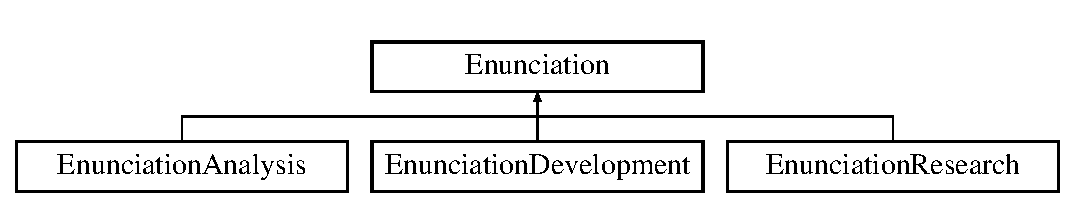
\includegraphics[height=2.000000cm]{class_enunciation}
\end{center}
\end{figure}
\subsection*{Public Member Functions}
\begin{DoxyCompactItemize}
\item 
\hyperlink{class_enunciation_a78a6f3656b8d057dfef51593de59193f}{Enunciation} ()
\begin{DoxyCompactList}\small\item\em Default constructor of \hyperlink{class_enunciation}{Enunciation} class. \end{DoxyCompactList}\item 
\hyperlink{class_enunciation_a954fa90c85714409ab224e6f405c26e4}{Enunciation} (string \hyperlink{class_enunciation_a5e2accd01df4c81578dc8f7b83507167}{title}, string \hyperlink{class_enunciation_a0b30051b66bd07b227f6a227befb6c0c}{description})
\begin{DoxyCompactList}\small\item\em Custom constructor of \hyperlink{class_enunciation}{Enunciation} class. \end{DoxyCompactList}\item 
string \hyperlink{class_enunciation_a7db0b7bc585b133d7faae9a7a8f78be6}{get\+Title} () const
\item 
string \hyperlink{class_enunciation_a8f5a6300cf6eb691ca1600191bf20e5e}{get\+Description} () const
\item 
void \hyperlink{class_enunciation_a84cebe1417311997307664608305b305}{set\+Title} (string new\+Title)
\begin{DoxyCompactList}\small\item\em Sets a new title for the enunciation associated. \end{DoxyCompactList}\item 
void \hyperlink{class_enunciation_ae3a90d3e7ed1072d44c9801c689aa08f}{set\+Description} (string new\+Description)
\begin{DoxyCompactList}\small\item\em Sets a new description for the enunciation associated. \end{DoxyCompactList}\item 
void \hyperlink{class_enunciation_a86a3547dd604f7050a5e12b473ba6eef}{add\+Year} (\hyperlink{class_occurrence}{Occurrence} $\ast$new\+Year)
\begin{DoxyCompactList}\small\item\em Adds a new year to the occurrences vector. \end{DoxyCompactList}\item 
vector$<$ \hyperlink{class_occurrence}{Occurrence} $\ast$ $>$ \hyperlink{class_enunciation_a8fe49ff095b219adb6841976b8983ebe}{get\+Occurrences} () const
\item 
virtual string \hyperlink{class_enunciation_a032b5ff494595ab52d152d605544525c}{get\+Info} ()
\begin{DoxyCompactList}\small\item\em Virtual function to get information of a certain enunciation. \end{DoxyCompactList}\item 
virtual string \hyperlink{class_enunciation_a2c27d4c83302dd7d21e1064c9e4ec97d}{get\+Code} ()
\begin{DoxyCompactList}\small\item\em Virtual function to get code of a certain enunciation. \end{DoxyCompactList}\item 
virtual string \hyperlink{class_enunciation_ad0bf6d8d34f6246cd5bc674b15b5958b}{get\+Addition} ()
\begin{DoxyCompactList}\small\item\em Virtual function to get addition of a certain enunciation. \end{DoxyCompactList}\item 
void \hyperlink{class_enunciation_a1ae5e84684d7aea08b888836661c0a01}{sort\+Occurrences} ()
\begin{DoxyCompactList}\small\item\em Sorts occurrences. \end{DoxyCompactList}\end{DoxyCompactItemize}
\subsection*{Protected Attributes}
\begin{DoxyCompactItemize}
\item 
string \hyperlink{class_enunciation_a5e2accd01df4c81578dc8f7b83507167}{title}
\item 
string \hyperlink{class_enunciation_a0b30051b66bd07b227f6a227befb6c0c}{description}
\item 
vector$<$ \hyperlink{class_occurrence}{Occurrence} $\ast$ $>$ \hyperlink{class_enunciation_a54cce81b8d17a0e2f06d651988507a4a}{years}
\end{DoxyCompactItemize}


\subsection{Constructor \& Destructor Documentation}
\mbox{\Hypertarget{class_enunciation_a78a6f3656b8d057dfef51593de59193f}\label{class_enunciation_a78a6f3656b8d057dfef51593de59193f}} 
\index{Enunciation@{Enunciation}!Enunciation@{Enunciation}}
\index{Enunciation@{Enunciation}!Enunciation@{Enunciation}}
\subsubsection{\texorpdfstring{Enunciation()}{Enunciation()}\hspace{0.1cm}{\footnotesize\ttfamily [1/2]}}
{\footnotesize\ttfamily Enunciation\+::\+Enunciation (\begin{DoxyParamCaption}{ }\end{DoxyParamCaption})}



Default constructor of \hyperlink{class_enunciation}{Enunciation} class. 

\mbox{\Hypertarget{class_enunciation_a954fa90c85714409ab224e6f405c26e4}\label{class_enunciation_a954fa90c85714409ab224e6f405c26e4}} 
\index{Enunciation@{Enunciation}!Enunciation@{Enunciation}}
\index{Enunciation@{Enunciation}!Enunciation@{Enunciation}}
\subsubsection{\texorpdfstring{Enunciation()}{Enunciation()}\hspace{0.1cm}{\footnotesize\ttfamily [2/2]}}
{\footnotesize\ttfamily Enunciation\+::\+Enunciation (\begin{DoxyParamCaption}\item[{string}]{title,  }\item[{string}]{description }\end{DoxyParamCaption})}



Custom constructor of \hyperlink{class_enunciation}{Enunciation} class. 


\begin{DoxyParams}{Parameters}
{\em title} & Title of the enunciation \\
\hline
{\em description} & Description of that enunciation \\
\hline
\end{DoxyParams}


\subsection{Member Function Documentation}
\mbox{\Hypertarget{class_enunciation_a86a3547dd604f7050a5e12b473ba6eef}\label{class_enunciation_a86a3547dd604f7050a5e12b473ba6eef}} 
\index{Enunciation@{Enunciation}!add\+Year@{add\+Year}}
\index{add\+Year@{add\+Year}!Enunciation@{Enunciation}}
\subsubsection{\texorpdfstring{add\+Year()}{addYear()}}
{\footnotesize\ttfamily void Enunciation\+::add\+Year (\begin{DoxyParamCaption}\item[{\hyperlink{class_occurrence}{Occurrence} $\ast$}]{new\+Year }\end{DoxyParamCaption})}



Adds a new year to the occurrences vector. 


\begin{DoxyParams}{Parameters}
{\em new\+Year} & Pointer to the new \hyperlink{class_occurrence}{Occurrence} to be added \\
\hline
\end{DoxyParams}
\mbox{\Hypertarget{class_enunciation_ad0bf6d8d34f6246cd5bc674b15b5958b}\label{class_enunciation_ad0bf6d8d34f6246cd5bc674b15b5958b}} 
\index{Enunciation@{Enunciation}!get\+Addition@{get\+Addition}}
\index{get\+Addition@{get\+Addition}!Enunciation@{Enunciation}}
\subsubsection{\texorpdfstring{get\+Addition()}{getAddition()}}
{\footnotesize\ttfamily string Enunciation\+::get\+Addition (\begin{DoxyParamCaption}{ }\end{DoxyParamCaption})\hspace{0.3cm}{\ttfamily [virtual]}}



Virtual function to get addition of a certain enunciation. 



Reimplemented in \hyperlink{class_enunciation_development_a5480d39ba25c6fac36d07d3aad6b6de9}{Enunciation\+Development}, \hyperlink{class_enunciation_analysis_a19fa90c811af4addfe77c4109520a8e1}{Enunciation\+Analysis}, and \hyperlink{class_enunciation_research_ad5021c15b3cf600191d21aec467529d4}{Enunciation\+Research}.

\mbox{\Hypertarget{class_enunciation_a2c27d4c83302dd7d21e1064c9e4ec97d}\label{class_enunciation_a2c27d4c83302dd7d21e1064c9e4ec97d}} 
\index{Enunciation@{Enunciation}!get\+Code@{get\+Code}}
\index{get\+Code@{get\+Code}!Enunciation@{Enunciation}}
\subsubsection{\texorpdfstring{get\+Code()}{getCode()}}
{\footnotesize\ttfamily string Enunciation\+::get\+Code (\begin{DoxyParamCaption}{ }\end{DoxyParamCaption})\hspace{0.3cm}{\ttfamily [virtual]}}



Virtual function to get code of a certain enunciation. 



Reimplemented in \hyperlink{class_enunciation_development_aa0e2d2c396cc3ec68df31334ae475850}{Enunciation\+Development}, \hyperlink{class_enunciation_analysis_a8393cb5e4c7a096f09e1112dbc854cf8}{Enunciation\+Analysis}, and \hyperlink{class_enunciation_research_a424e392956c1c7bbccfdf74d72b3d4dd}{Enunciation\+Research}.

\mbox{\Hypertarget{class_enunciation_a8f5a6300cf6eb691ca1600191bf20e5e}\label{class_enunciation_a8f5a6300cf6eb691ca1600191bf20e5e}} 
\index{Enunciation@{Enunciation}!get\+Description@{get\+Description}}
\index{get\+Description@{get\+Description}!Enunciation@{Enunciation}}
\subsubsection{\texorpdfstring{get\+Description()}{getDescription()}}
{\footnotesize\ttfamily string Enunciation\+::get\+Description (\begin{DoxyParamCaption}{ }\end{DoxyParamCaption}) const}

\begin{DoxyReturn}{Returns}
The description of the enunciation 
\end{DoxyReturn}
\mbox{\Hypertarget{class_enunciation_a032b5ff494595ab52d152d605544525c}\label{class_enunciation_a032b5ff494595ab52d152d605544525c}} 
\index{Enunciation@{Enunciation}!get\+Info@{get\+Info}}
\index{get\+Info@{get\+Info}!Enunciation@{Enunciation}}
\subsubsection{\texorpdfstring{get\+Info()}{getInfo()}}
{\footnotesize\ttfamily string Enunciation\+::get\+Info (\begin{DoxyParamCaption}{ }\end{DoxyParamCaption})\hspace{0.3cm}{\ttfamily [virtual]}}



Virtual function to get information of a certain enunciation. 



Reimplemented in \hyperlink{class_enunciation_development_a06289f811338e030977e59f083c618b6}{Enunciation\+Development}, \hyperlink{class_enunciation_analysis_a6cc8894f92eecbb68a7ebeb4a8365896}{Enunciation\+Analysis}, and \hyperlink{class_enunciation_research_a57ce30430703246bdd6a1103530a8a5f}{Enunciation\+Research}.

\mbox{\Hypertarget{class_enunciation_a8fe49ff095b219adb6841976b8983ebe}\label{class_enunciation_a8fe49ff095b219adb6841976b8983ebe}} 
\index{Enunciation@{Enunciation}!get\+Occurrences@{get\+Occurrences}}
\index{get\+Occurrences@{get\+Occurrences}!Enunciation@{Enunciation}}
\subsubsection{\texorpdfstring{get\+Occurrences()}{getOccurrences()}}
{\footnotesize\ttfamily vector$<$ \hyperlink{class_occurrence}{Occurrence} $\ast$ $>$ Enunciation\+::get\+Occurrences (\begin{DoxyParamCaption}{ }\end{DoxyParamCaption}) const}

\begin{DoxyReturn}{Returns}
The ocurrences of an enunciation 
\end{DoxyReturn}
\mbox{\Hypertarget{class_enunciation_a7db0b7bc585b133d7faae9a7a8f78be6}\label{class_enunciation_a7db0b7bc585b133d7faae9a7a8f78be6}} 
\index{Enunciation@{Enunciation}!get\+Title@{get\+Title}}
\index{get\+Title@{get\+Title}!Enunciation@{Enunciation}}
\subsubsection{\texorpdfstring{get\+Title()}{getTitle()}}
{\footnotesize\ttfamily string Enunciation\+::get\+Title (\begin{DoxyParamCaption}{ }\end{DoxyParamCaption}) const}

\begin{DoxyReturn}{Returns}
Gets the title of the enunciation 
\end{DoxyReturn}
\mbox{\Hypertarget{class_enunciation_ae3a90d3e7ed1072d44c9801c689aa08f}\label{class_enunciation_ae3a90d3e7ed1072d44c9801c689aa08f}} 
\index{Enunciation@{Enunciation}!set\+Description@{set\+Description}}
\index{set\+Description@{set\+Description}!Enunciation@{Enunciation}}
\subsubsection{\texorpdfstring{set\+Description()}{setDescription()}}
{\footnotesize\ttfamily void Enunciation\+::set\+Description (\begin{DoxyParamCaption}\item[{string}]{new\+Description }\end{DoxyParamCaption})}



Sets a new description for the enunciation associated. 


\begin{DoxyParams}{Parameters}
{\em new\+Description} & The new description \\
\hline
\end{DoxyParams}
\mbox{\Hypertarget{class_enunciation_a84cebe1417311997307664608305b305}\label{class_enunciation_a84cebe1417311997307664608305b305}} 
\index{Enunciation@{Enunciation}!set\+Title@{set\+Title}}
\index{set\+Title@{set\+Title}!Enunciation@{Enunciation}}
\subsubsection{\texorpdfstring{set\+Title()}{setTitle()}}
{\footnotesize\ttfamily void Enunciation\+::set\+Title (\begin{DoxyParamCaption}\item[{string}]{new\+Title }\end{DoxyParamCaption})}



Sets a new title for the enunciation associated. 


\begin{DoxyParams}{Parameters}
{\em new\+Title} & The new title \\
\hline
\end{DoxyParams}
\mbox{\Hypertarget{class_enunciation_a1ae5e84684d7aea08b888836661c0a01}\label{class_enunciation_a1ae5e84684d7aea08b888836661c0a01}} 
\index{Enunciation@{Enunciation}!sort\+Occurrences@{sort\+Occurrences}}
\index{sort\+Occurrences@{sort\+Occurrences}!Enunciation@{Enunciation}}
\subsubsection{\texorpdfstring{sort\+Occurrences()}{sortOccurrences()}}
{\footnotesize\ttfamily void Enunciation\+::sort\+Occurrences (\begin{DoxyParamCaption}{ }\end{DoxyParamCaption})}



Sorts occurrences. 



\subsection{Member Data Documentation}
\mbox{\Hypertarget{class_enunciation_a0b30051b66bd07b227f6a227befb6c0c}\label{class_enunciation_a0b30051b66bd07b227f6a227befb6c0c}} 
\index{Enunciation@{Enunciation}!description@{description}}
\index{description@{description}!Enunciation@{Enunciation}}
\subsubsection{\texorpdfstring{description}{description}}
{\footnotesize\ttfamily string Enunciation\+::description\hspace{0.3cm}{\ttfamily [protected]}}

\mbox{\Hypertarget{class_enunciation_a5e2accd01df4c81578dc8f7b83507167}\label{class_enunciation_a5e2accd01df4c81578dc8f7b83507167}} 
\index{Enunciation@{Enunciation}!title@{title}}
\index{title@{title}!Enunciation@{Enunciation}}
\subsubsection{\texorpdfstring{title}{title}}
{\footnotesize\ttfamily string Enunciation\+::title\hspace{0.3cm}{\ttfamily [protected]}}

\mbox{\Hypertarget{class_enunciation_a54cce81b8d17a0e2f06d651988507a4a}\label{class_enunciation_a54cce81b8d17a0e2f06d651988507a4a}} 
\index{Enunciation@{Enunciation}!years@{years}}
\index{years@{years}!Enunciation@{Enunciation}}
\subsubsection{\texorpdfstring{years}{years}}
{\footnotesize\ttfamily vector$<$\hyperlink{class_occurrence}{Occurrence} $\ast$$>$ Enunciation\+::years\hspace{0.3cm}{\ttfamily [protected]}}



The documentation for this class was generated from the following files\+:\begin{DoxyCompactItemize}
\item 
\hyperlink{enunciation_8h}{enunciation.\+h}\item 
\hyperlink{enunciation_8cpp}{enunciation.\+cpp}\end{DoxyCompactItemize}

\hypertarget{class_enunciation_analysis}{}\section{Enunciation\+Analysis Class Reference}
\label{class_enunciation_analysis}\index{Enunciation\+Analysis@{Enunciation\+Analysis}}


{\ttfamily \#include $<$enunciation.\+h$>$}

Inheritance diagram for Enunciation\+Analysis\+:\begin{figure}[H]
\begin{center}
\leavevmode
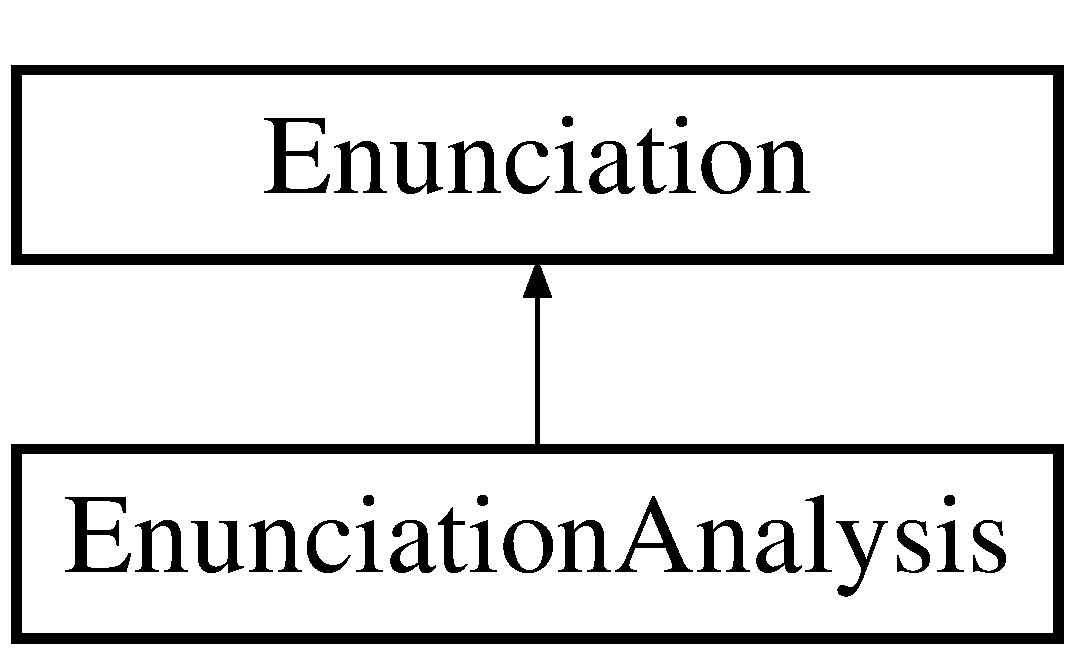
\includegraphics[height=2.000000cm]{class_enunciation_analysis}
\end{center}
\end{figure}
\subsection*{Public Member Functions}
\begin{DoxyCompactItemize}
\item 
\hyperlink{class_enunciation_analysis_a1a6a72d187591dd38fbf92a37fee22dc}{Enunciation\+Analysis} (string \hyperlink{class_enunciation_a5e2accd01df4c81578dc8f7b83507167}{title}, string \hyperlink{class_enunciation_a0b30051b66bd07b227f6a227befb6c0c}{description})
\begin{DoxyCompactList}\small\item\em Custom constructor of \hyperlink{class_enunciation_analysis}{Enunciation\+Analysis} class. \end{DoxyCompactList}\item 
string \hyperlink{class_enunciation_analysis_a19fa90c811af4addfe77c4109520a8e1}{get\+Addition} ()
\begin{DoxyCompactList}\small\item\em Virtual function to get addition of a certain enunciation. \end{DoxyCompactList}\item 
void \hyperlink{class_enunciation_analysis_a5529f1e325fab32099b8845a2b624fa7}{set\+Repos} (string \hyperlink{class_enunciation_analysis_a3ceb48cf1cfe6594b853b52c9ce9aae4}{repos})
\begin{DoxyCompactList}\small\item\em Sets a new repository for the enunciation. \end{DoxyCompactList}\item 
string \hyperlink{class_enunciation_analysis_a6cc8894f92eecbb68a7ebeb4a8365896}{get\+Info} ()
\item 
string \hyperlink{class_enunciation_analysis_a8393cb5e4c7a096f09e1112dbc854cf8}{get\+Code} ()
\end{DoxyCompactItemize}
\subsection*{Protected Attributes}
\begin{DoxyCompactItemize}
\item 
string \hyperlink{class_enunciation_analysis_a3ceb48cf1cfe6594b853b52c9ce9aae4}{repos}
\end{DoxyCompactItemize}


\subsection{Constructor \& Destructor Documentation}
\mbox{\Hypertarget{class_enunciation_analysis_a1a6a72d187591dd38fbf92a37fee22dc}\label{class_enunciation_analysis_a1a6a72d187591dd38fbf92a37fee22dc}} 
\index{Enunciation\+Analysis@{Enunciation\+Analysis}!Enunciation\+Analysis@{Enunciation\+Analysis}}
\index{Enunciation\+Analysis@{Enunciation\+Analysis}!Enunciation\+Analysis@{Enunciation\+Analysis}}
\subsubsection{\texorpdfstring{Enunciation\+Analysis()}{EnunciationAnalysis()}}
{\footnotesize\ttfamily Enunciation\+Analysis\+::\+Enunciation\+Analysis (\begin{DoxyParamCaption}\item[{string}]{title,  }\item[{string}]{description }\end{DoxyParamCaption})}



Custom constructor of \hyperlink{class_enunciation_analysis}{Enunciation\+Analysis} class. 


\begin{DoxyParams}{Parameters}
{\em title} & Title of the enunciation \\
\hline
{\em description} & Description of that enunciation \\
\hline
\end{DoxyParams}


\subsection{Member Function Documentation}
\mbox{\Hypertarget{class_enunciation_analysis_a19fa90c811af4addfe77c4109520a8e1}\label{class_enunciation_analysis_a19fa90c811af4addfe77c4109520a8e1}} 
\index{Enunciation\+Analysis@{Enunciation\+Analysis}!get\+Addition@{get\+Addition}}
\index{get\+Addition@{get\+Addition}!Enunciation\+Analysis@{Enunciation\+Analysis}}
\subsubsection{\texorpdfstring{get\+Addition()}{getAddition()}}
{\footnotesize\ttfamily string Enunciation\+Analysis\+::get\+Addition (\begin{DoxyParamCaption}{ }\end{DoxyParamCaption})\hspace{0.3cm}{\ttfamily [virtual]}}



Virtual function to get addition of a certain enunciation. 



Reimplemented from \hyperlink{class_enunciation_ad0bf6d8d34f6246cd5bc674b15b5958b}{Enunciation}.

\mbox{\Hypertarget{class_enunciation_analysis_a8393cb5e4c7a096f09e1112dbc854cf8}\label{class_enunciation_analysis_a8393cb5e4c7a096f09e1112dbc854cf8}} 
\index{Enunciation\+Analysis@{Enunciation\+Analysis}!get\+Code@{get\+Code}}
\index{get\+Code@{get\+Code}!Enunciation\+Analysis@{Enunciation\+Analysis}}
\subsubsection{\texorpdfstring{get\+Code()}{getCode()}}
{\footnotesize\ttfamily string Enunciation\+Analysis\+::get\+Code (\begin{DoxyParamCaption}{ }\end{DoxyParamCaption})\hspace{0.3cm}{\ttfamily [virtual]}}

\begin{DoxyReturn}{Returns}
Code about an enunciation 
\end{DoxyReturn}


Reimplemented from \hyperlink{class_enunciation_a2c27d4c83302dd7d21e1064c9e4ec97d}{Enunciation}.

\mbox{\Hypertarget{class_enunciation_analysis_a6cc8894f92eecbb68a7ebeb4a8365896}\label{class_enunciation_analysis_a6cc8894f92eecbb68a7ebeb4a8365896}} 
\index{Enunciation\+Analysis@{Enunciation\+Analysis}!get\+Info@{get\+Info}}
\index{get\+Info@{get\+Info}!Enunciation\+Analysis@{Enunciation\+Analysis}}
\subsubsection{\texorpdfstring{get\+Info()}{getInfo()}}
{\footnotesize\ttfamily string Enunciation\+Analysis\+::get\+Info (\begin{DoxyParamCaption}{ }\end{DoxyParamCaption})\hspace{0.3cm}{\ttfamily [virtual]}}

\begin{DoxyReturn}{Returns}
Information about an enunciation 
\end{DoxyReturn}


Reimplemented from \hyperlink{class_enunciation_a032b5ff494595ab52d152d605544525c}{Enunciation}.

\mbox{\Hypertarget{class_enunciation_analysis_a5529f1e325fab32099b8845a2b624fa7}\label{class_enunciation_analysis_a5529f1e325fab32099b8845a2b624fa7}} 
\index{Enunciation\+Analysis@{Enunciation\+Analysis}!set\+Repos@{set\+Repos}}
\index{set\+Repos@{set\+Repos}!Enunciation\+Analysis@{Enunciation\+Analysis}}
\subsubsection{\texorpdfstring{set\+Repos()}{setRepos()}}
{\footnotesize\ttfamily void Enunciation\+Analysis\+::set\+Repos (\begin{DoxyParamCaption}\item[{string}]{repos }\end{DoxyParamCaption})}



Sets a new repository for the enunciation. 


\begin{DoxyParams}{Parameters}
{\em repos} & The new repository \\
\hline
\end{DoxyParams}


\subsection{Member Data Documentation}
\mbox{\Hypertarget{class_enunciation_analysis_a3ceb48cf1cfe6594b853b52c9ce9aae4}\label{class_enunciation_analysis_a3ceb48cf1cfe6594b853b52c9ce9aae4}} 
\index{Enunciation\+Analysis@{Enunciation\+Analysis}!repos@{repos}}
\index{repos@{repos}!Enunciation\+Analysis@{Enunciation\+Analysis}}
\subsubsection{\texorpdfstring{repos}{repos}}
{\footnotesize\ttfamily string Enunciation\+Analysis\+::repos\hspace{0.3cm}{\ttfamily [protected]}}



The documentation for this class was generated from the following files\+:\begin{DoxyCompactItemize}
\item 
\hyperlink{enunciation_8h}{enunciation.\+h}\item 
\hyperlink{enunciation_8cpp}{enunciation.\+cpp}\end{DoxyCompactItemize}

\hypertarget{class_enunciation_development}{}\section{Enunciation\+Development Class Reference}
\label{class_enunciation_development}\index{Enunciation\+Development@{Enunciation\+Development}}


{\ttfamily \#include $<$enunciation.\+h$>$}

Inheritance diagram for Enunciation\+Development\+:\begin{figure}[H]
\begin{center}
\leavevmode
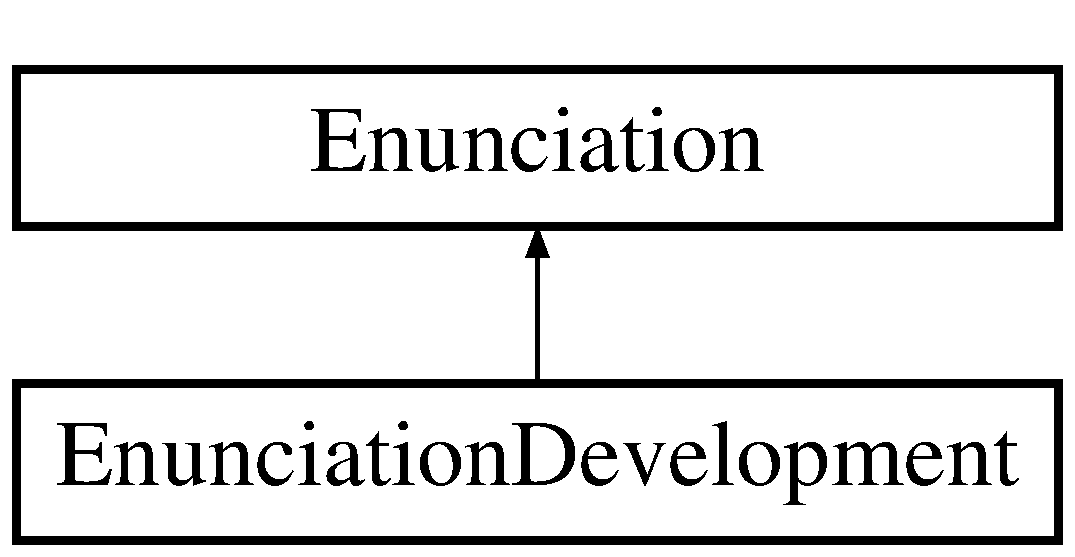
\includegraphics[height=2.000000cm]{class_enunciation_development}
\end{center}
\end{figure}
\subsection*{Public Member Functions}
\begin{DoxyCompactItemize}
\item 
\hyperlink{class_enunciation_development_a8846729f4e511003b416a58cf580c9ff}{Enunciation\+Development} (string \hyperlink{class_enunciation_a5e2accd01df4c81578dc8f7b83507167}{title}, string \hyperlink{class_enunciation_a0b30051b66bd07b227f6a227befb6c0c}{description})
\begin{DoxyCompactList}\small\item\em Custom constructor of \hyperlink{class_enunciation_development}{Enunciation\+Development} class. \end{DoxyCompactList}\item 
string \hyperlink{class_enunciation_development_a5480d39ba25c6fac36d07d3aad6b6de9}{get\+Addition} ()
\begin{DoxyCompactList}\small\item\em Virtual function to get addition of a certain enunciation. \end{DoxyCompactList}\item 
void \hyperlink{class_enunciation_development_afeefc36344ab2cf3949e9bcc9e9f839b}{set\+Result} (string \hyperlink{class_enunciation_development_abc152492be3a1049b84b581022f0bf6f}{results})
\begin{DoxyCompactList}\small\item\em Sets a new result for the enunciation. \end{DoxyCompactList}\item 
string \hyperlink{class_enunciation_development_a06289f811338e030977e59f083c618b6}{get\+Info} ()
\item 
string \hyperlink{class_enunciation_development_aa0e2d2c396cc3ec68df31334ae475850}{get\+Code} ()
\end{DoxyCompactItemize}
\subsection*{Protected Attributes}
\begin{DoxyCompactItemize}
\item 
string \hyperlink{class_enunciation_development_abc152492be3a1049b84b581022f0bf6f}{results}
\end{DoxyCompactItemize}


\subsection{Constructor \& Destructor Documentation}
\mbox{\Hypertarget{class_enunciation_development_a8846729f4e511003b416a58cf580c9ff}\label{class_enunciation_development_a8846729f4e511003b416a58cf580c9ff}} 
\index{Enunciation\+Development@{Enunciation\+Development}!Enunciation\+Development@{Enunciation\+Development}}
\index{Enunciation\+Development@{Enunciation\+Development}!Enunciation\+Development@{Enunciation\+Development}}
\subsubsection{\texorpdfstring{Enunciation\+Development()}{EnunciationDevelopment()}}
{\footnotesize\ttfamily Enunciation\+Development\+::\+Enunciation\+Development (\begin{DoxyParamCaption}\item[{string}]{title,  }\item[{string}]{description }\end{DoxyParamCaption})}



Custom constructor of \hyperlink{class_enunciation_development}{Enunciation\+Development} class. 


\begin{DoxyParams}{Parameters}
{\em title} & Title of the enunciation \\
\hline
{\em description} & Description of that enunciation \\
\hline
\end{DoxyParams}


\subsection{Member Function Documentation}
\mbox{\Hypertarget{class_enunciation_development_a5480d39ba25c6fac36d07d3aad6b6de9}\label{class_enunciation_development_a5480d39ba25c6fac36d07d3aad6b6de9}} 
\index{Enunciation\+Development@{Enunciation\+Development}!get\+Addition@{get\+Addition}}
\index{get\+Addition@{get\+Addition}!Enunciation\+Development@{Enunciation\+Development}}
\subsubsection{\texorpdfstring{get\+Addition()}{getAddition()}}
{\footnotesize\ttfamily string Enunciation\+Development\+::get\+Addition (\begin{DoxyParamCaption}{ }\end{DoxyParamCaption})\hspace{0.3cm}{\ttfamily [virtual]}}



Virtual function to get addition of a certain enunciation. 



Reimplemented from \hyperlink{class_enunciation_ad0bf6d8d34f6246cd5bc674b15b5958b}{Enunciation}.

\mbox{\Hypertarget{class_enunciation_development_aa0e2d2c396cc3ec68df31334ae475850}\label{class_enunciation_development_aa0e2d2c396cc3ec68df31334ae475850}} 
\index{Enunciation\+Development@{Enunciation\+Development}!get\+Code@{get\+Code}}
\index{get\+Code@{get\+Code}!Enunciation\+Development@{Enunciation\+Development}}
\subsubsection{\texorpdfstring{get\+Code()}{getCode()}}
{\footnotesize\ttfamily string Enunciation\+Development\+::get\+Code (\begin{DoxyParamCaption}{ }\end{DoxyParamCaption})\hspace{0.3cm}{\ttfamily [virtual]}}

\begin{DoxyReturn}{Returns}
Code about an enunciation 
\end{DoxyReturn}


Reimplemented from \hyperlink{class_enunciation_a2c27d4c83302dd7d21e1064c9e4ec97d}{Enunciation}.

\mbox{\Hypertarget{class_enunciation_development_a06289f811338e030977e59f083c618b6}\label{class_enunciation_development_a06289f811338e030977e59f083c618b6}} 
\index{Enunciation\+Development@{Enunciation\+Development}!get\+Info@{get\+Info}}
\index{get\+Info@{get\+Info}!Enunciation\+Development@{Enunciation\+Development}}
\subsubsection{\texorpdfstring{get\+Info()}{getInfo()}}
{\footnotesize\ttfamily string Enunciation\+Development\+::get\+Info (\begin{DoxyParamCaption}{ }\end{DoxyParamCaption})\hspace{0.3cm}{\ttfamily [virtual]}}

\begin{DoxyReturn}{Returns}
Information about an enunciation 
\end{DoxyReturn}


Reimplemented from \hyperlink{class_enunciation_a032b5ff494595ab52d152d605544525c}{Enunciation}.

\mbox{\Hypertarget{class_enunciation_development_afeefc36344ab2cf3949e9bcc9e9f839b}\label{class_enunciation_development_afeefc36344ab2cf3949e9bcc9e9f839b}} 
\index{Enunciation\+Development@{Enunciation\+Development}!set\+Result@{set\+Result}}
\index{set\+Result@{set\+Result}!Enunciation\+Development@{Enunciation\+Development}}
\subsubsection{\texorpdfstring{set\+Result()}{setResult()}}
{\footnotesize\ttfamily void Enunciation\+Development\+::set\+Result (\begin{DoxyParamCaption}\item[{string}]{results }\end{DoxyParamCaption})}



Sets a new result for the enunciation. 


\begin{DoxyParams}{Parameters}
{\em results} & The new results \\
\hline
\end{DoxyParams}


\subsection{Member Data Documentation}
\mbox{\Hypertarget{class_enunciation_development_abc152492be3a1049b84b581022f0bf6f}\label{class_enunciation_development_abc152492be3a1049b84b581022f0bf6f}} 
\index{Enunciation\+Development@{Enunciation\+Development}!results@{results}}
\index{results@{results}!Enunciation\+Development@{Enunciation\+Development}}
\subsubsection{\texorpdfstring{results}{results}}
{\footnotesize\ttfamily string Enunciation\+Development\+::results\hspace{0.3cm}{\ttfamily [protected]}}



The documentation for this class was generated from the following files\+:\begin{DoxyCompactItemize}
\item 
\hyperlink{enunciation_8h}{enunciation.\+h}\item 
\hyperlink{enunciation_8cpp}{enunciation.\+cpp}\end{DoxyCompactItemize}

\hypertarget{class_enunciation_research}{}\section{Enunciation\+Research Class Reference}
\label{class_enunciation_research}\index{Enunciation\+Research@{Enunciation\+Research}}


{\ttfamily \#include $<$enunciation.\+h$>$}

Inheritance diagram for Enunciation\+Research\+:\begin{figure}[H]
\begin{center}
\leavevmode
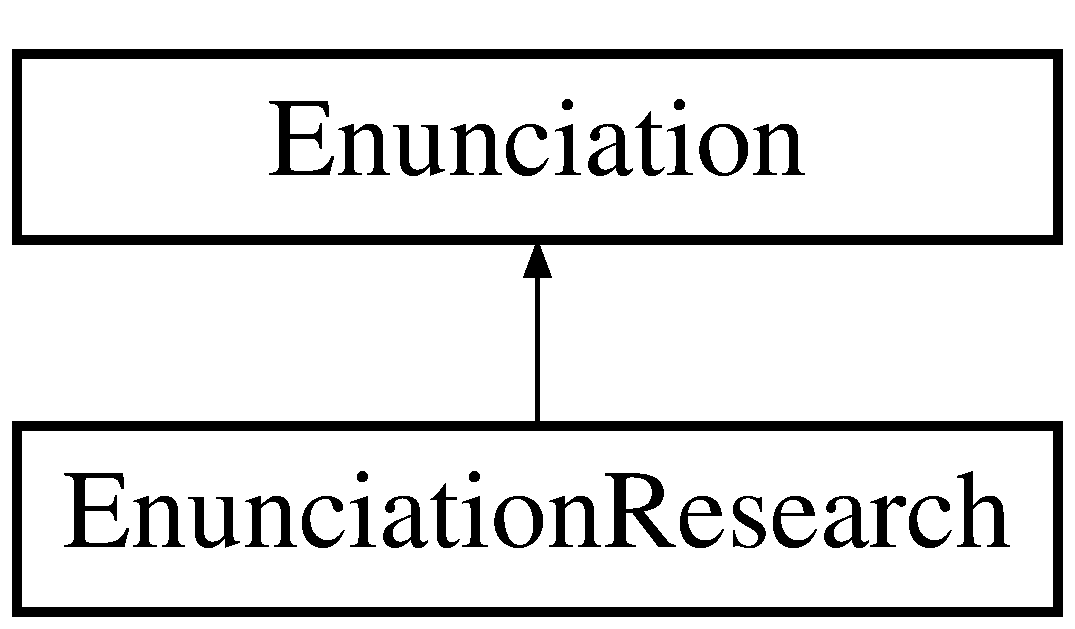
\includegraphics[height=2.000000cm]{class_enunciation_research}
\end{center}
\end{figure}
\subsection*{Public Member Functions}
\begin{DoxyCompactItemize}
\item 
\hyperlink{class_enunciation_research_ac5d9450c0cdd0c2682e7b2ba35ca1258}{Enunciation\+Research} (string \hyperlink{class_enunciation_a5e2accd01df4c81578dc8f7b83507167}{title}, string \hyperlink{class_enunciation_a0b30051b66bd07b227f6a227befb6c0c}{description})
\begin{DoxyCompactList}\small\item\em Custom constructor of \hyperlink{class_enunciation_research}{Enunciation\+Research} class. \end{DoxyCompactList}\item 
string \hyperlink{class_enunciation_research_ad5021c15b3cf600191d21aec467529d4}{get\+Addition} ()
\begin{DoxyCompactList}\small\item\em Virtual function to get addition of a certain enunciation. \end{DoxyCompactList}\item 
void \hyperlink{class_enunciation_research_afc23a08d1cce9f77f64c664614f7a4fc}{set\+Biblio} (string \hyperlink{class_enunciation_research_a425da04eb657de83211819d1af3fc640}{biblio})
\begin{DoxyCompactList}\small\item\em Sets a new biblio for the enunciation. \end{DoxyCompactList}\item 
string \hyperlink{class_enunciation_research_a57ce30430703246bdd6a1103530a8a5f}{get\+Info} ()
\item 
string \hyperlink{class_enunciation_research_a424e392956c1c7bbccfdf74d72b3d4dd}{get\+Code} ()
\end{DoxyCompactItemize}
\subsection*{Protected Attributes}
\begin{DoxyCompactItemize}
\item 
string \hyperlink{class_enunciation_research_a425da04eb657de83211819d1af3fc640}{biblio}
\end{DoxyCompactItemize}


\subsection{Constructor \& Destructor Documentation}
\mbox{\Hypertarget{class_enunciation_research_ac5d9450c0cdd0c2682e7b2ba35ca1258}\label{class_enunciation_research_ac5d9450c0cdd0c2682e7b2ba35ca1258}} 
\index{Enunciation\+Research@{Enunciation\+Research}!Enunciation\+Research@{Enunciation\+Research}}
\index{Enunciation\+Research@{Enunciation\+Research}!Enunciation\+Research@{Enunciation\+Research}}
\subsubsection{\texorpdfstring{Enunciation\+Research()}{EnunciationResearch()}}
{\footnotesize\ttfamily Enunciation\+Research\+::\+Enunciation\+Research (\begin{DoxyParamCaption}\item[{string}]{title,  }\item[{string}]{description }\end{DoxyParamCaption})}



Custom constructor of \hyperlink{class_enunciation_research}{Enunciation\+Research} class. 


\begin{DoxyParams}{Parameters}
{\em title} & Title of the enunciation \\
\hline
{\em description} & Description of that enunciation \\
\hline
\end{DoxyParams}


\subsection{Member Function Documentation}
\mbox{\Hypertarget{class_enunciation_research_ad5021c15b3cf600191d21aec467529d4}\label{class_enunciation_research_ad5021c15b3cf600191d21aec467529d4}} 
\index{Enunciation\+Research@{Enunciation\+Research}!get\+Addition@{get\+Addition}}
\index{get\+Addition@{get\+Addition}!Enunciation\+Research@{Enunciation\+Research}}
\subsubsection{\texorpdfstring{get\+Addition()}{getAddition()}}
{\footnotesize\ttfamily string Enunciation\+Research\+::get\+Addition (\begin{DoxyParamCaption}{ }\end{DoxyParamCaption})\hspace{0.3cm}{\ttfamily [virtual]}}



Virtual function to get addition of a certain enunciation. 



Reimplemented from \hyperlink{class_enunciation_ad0bf6d8d34f6246cd5bc674b15b5958b}{Enunciation}.

\mbox{\Hypertarget{class_enunciation_research_a424e392956c1c7bbccfdf74d72b3d4dd}\label{class_enunciation_research_a424e392956c1c7bbccfdf74d72b3d4dd}} 
\index{Enunciation\+Research@{Enunciation\+Research}!get\+Code@{get\+Code}}
\index{get\+Code@{get\+Code}!Enunciation\+Research@{Enunciation\+Research}}
\subsubsection{\texorpdfstring{get\+Code()}{getCode()}}
{\footnotesize\ttfamily string Enunciation\+Research\+::get\+Code (\begin{DoxyParamCaption}{ }\end{DoxyParamCaption})\hspace{0.3cm}{\ttfamily [virtual]}}

\begin{DoxyReturn}{Returns}
Code about an enunciation 
\end{DoxyReturn}


Reimplemented from \hyperlink{class_enunciation_a2c27d4c83302dd7d21e1064c9e4ec97d}{Enunciation}.

\mbox{\Hypertarget{class_enunciation_research_a57ce30430703246bdd6a1103530a8a5f}\label{class_enunciation_research_a57ce30430703246bdd6a1103530a8a5f}} 
\index{Enunciation\+Research@{Enunciation\+Research}!get\+Info@{get\+Info}}
\index{get\+Info@{get\+Info}!Enunciation\+Research@{Enunciation\+Research}}
\subsubsection{\texorpdfstring{get\+Info()}{getInfo()}}
{\footnotesize\ttfamily string Enunciation\+Research\+::get\+Info (\begin{DoxyParamCaption}{ }\end{DoxyParamCaption})\hspace{0.3cm}{\ttfamily [virtual]}}

\begin{DoxyReturn}{Returns}
Information about an enunciation 
\end{DoxyReturn}


Reimplemented from \hyperlink{class_enunciation_a032b5ff494595ab52d152d605544525c}{Enunciation}.

\mbox{\Hypertarget{class_enunciation_research_afc23a08d1cce9f77f64c664614f7a4fc}\label{class_enunciation_research_afc23a08d1cce9f77f64c664614f7a4fc}} 
\index{Enunciation\+Research@{Enunciation\+Research}!set\+Biblio@{set\+Biblio}}
\index{set\+Biblio@{set\+Biblio}!Enunciation\+Research@{Enunciation\+Research}}
\subsubsection{\texorpdfstring{set\+Biblio()}{setBiblio()}}
{\footnotesize\ttfamily void Enunciation\+Research\+::set\+Biblio (\begin{DoxyParamCaption}\item[{string}]{biblio }\end{DoxyParamCaption})}



Sets a new biblio for the enunciation. 


\begin{DoxyParams}{Parameters}
{\em biblio} & The new string biblio to be set \\
\hline
\end{DoxyParams}


\subsection{Member Data Documentation}
\mbox{\Hypertarget{class_enunciation_research_a425da04eb657de83211819d1af3fc640}\label{class_enunciation_research_a425da04eb657de83211819d1af3fc640}} 
\index{Enunciation\+Research@{Enunciation\+Research}!biblio@{biblio}}
\index{biblio@{biblio}!Enunciation\+Research@{Enunciation\+Research}}
\subsubsection{\texorpdfstring{biblio}{biblio}}
{\footnotesize\ttfamily string Enunciation\+Research\+::biblio\hspace{0.3cm}{\ttfamily [protected]}}



The documentation for this class was generated from the following files\+:\begin{DoxyCompactItemize}
\item 
\hyperlink{enunciation_8h}{enunciation.\+h}\item 
\hyperlink{enunciation_8cpp}{enunciation.\+cpp}\end{DoxyCompactItemize}

\hypertarget{classgeneral}{}\section{general Class Reference}
\label{classgeneral}\index{general@{general}}
\subsection*{Public Member Functions}
\begin{DoxyCompactItemize}
\item 
\hyperlink{classgeneral_a2a4fcaecb7d07e416a1188dee4fee767}{general} ()
\item 
void \hyperlink{classgeneral_ae11e9494ad52be040c2142bcfcb0c941}{Main\+Menu} ()
\item 
bool \hyperlink{classgeneral_a172fa5be50f0483a784daf5efcf117bc}{verify\+Getline} (int init, int end, string input)
\item 
void \hyperlink{classgeneral_a3751bee24e91f6924c028e8bd64879a8}{browse\+Techers\+Student\+Menu} ()
\item 
void \hyperlink{classgeneral_a0d1a8211230c588f90fede86f9a2976a}{browse\+Enunciation\+Menu} ()
\item 
void \hyperlink{classgeneral_ad6daefa1c532dd391c0b6d8c135eaec9}{create\+Enunciation\+Menu} ()
\item 
void \hyperlink{classgeneral_a2e8fee17772bc0ac04febd375ef98828}{list\+Enunciations} (vector$<$ \hyperlink{class_enunciation}{Enunciation} $\ast$$>$ le)
\item 
void \hyperlink{classgeneral_aaccf7ec238e4fb8f4f2430631764e87d}{find\+Teacher} ()
\item 
void \hyperlink{classgeneral_a7afc234dd64c7d7aa6caa64fa3029c5c}{find\+Student} ()
\item 
void \hyperlink{classgeneral_aa665c4f70405eae43862283c8f1c4268}{list\+Students} ()
\item 
void \hyperlink{classgeneral_aff78b35c2e50ad021d061977c4add3d8}{list\+Teachers} ()
\item 
void \hyperlink{classgeneral_a56cd18e2da56b705bc537d1c8f5ba7cc}{add\+Teacher} ()
\item 
void \hyperlink{classgeneral_a981fdd9aa5bca7fc3b997e328eeb2f64}{add\+Student} ()
\item 
void \hyperlink{classgeneral_a474cd69b70294468f3f004d594803a1a}{create\+New\+Occurrence} (string title, string year)
\item 
bool \hyperlink{classgeneral_a1420e73bcdd612483c7ffb5cb065d452}{check\+Good\+Date\+Input} (string date)
\item 
void \hyperlink{classgeneral_a49c62bf38d045b169a808f573b55c40b}{store\+A\+L\+L\+Enunciations\+In\+File} ()
\item 
void \hyperlink{classgeneral_aed7661222e35553e6c652d1f3644a955}{store\+Unused\+Enunciations\+In\+File} ()
\item 
void \hyperlink{classgeneral_a38338ad571ea0a44cdb34820af61ec02}{read\+A\+L\+L\+Enunciations\+From\+File} ()
\item 
void \hyperlink{classgeneral_a7cb5fbad7377cb86c3407d61875afd2a}{read\+People\+From\+File} ()
\item 
void \hyperlink{classgeneral_aa8628016088fdb471f40243bbd7a90f7}{read\+Projects\+From\+File} ()
\item 
void \hyperlink{classgeneral_a724d4f6e483cb27fa54a1116586fb496}{read\+Unused\+Enunciations\+From\+File} ()
\item 
int \hyperlink{classgeneral_a54a8942cc87fc31ddc7b43fb377e99bf}{new\+Id} ()
\item 
void \hyperlink{classgeneral_aeb426428b9cdb3fb7d42f7b701ac9b96}{store\+People\+In\+File} ()
\item 
void \hyperlink{classgeneral_abb8bdb048ce85c2f098ee8b2ec57523e}{store\+Projects\+In\+File} ()
\item 
void \hyperlink{classgeneral_a26dad8e6e689397eecb104c55add42b6}{sort\+By\+Number\+Students\+Enunciations} ()
\item 
void \hyperlink{classgeneral_ab9d9a464535f3ddc2cfe7d475f5035fd}{enunciation\+Show} (\hyperlink{class_enunciation}{Enunciation} $\ast$en)
\item 
void \hyperlink{classgeneral_ad7b4b452a1817239e686790feaaebb75}{year\+Show} (\hyperlink{class_occurrence}{Occurrence} $\ast$year, string title)
\item 
void \hyperlink{classgeneral_a0b996c23458ece0c89d862c106dd862a}{project\+Show} (\hyperlink{classgroup_project}{group\+Project} $\ast$pr, string title, \hyperlink{class_occurrence}{Occurrence} $\ast$year)
\item 
void \hyperlink{classgeneral_a0a6fecb5fd726b346db53c3210cc8de6}{list\+Unused\+Enunciations} ()
\item 
void \hyperlink{classgeneral_a551a81d21f47c57dfff3ab05b834ea45}{list\+B\+S\+T\+Enunciations\+By\+Type} ()
\item 
void \hyperlink{classgeneral_a81fb58747c318f62bbd352e2a2bc31e0}{evaluate\+Enunciations} ()
\item 
void \hyperlink{classgeneral_abf69d2951e72f3d5197bedc1d4baf832}{find\+Last\+Project} ()
\item 
void \hyperlink{classgeneral_aaecf57259d31156270464e3b738ad54a}{browse\+G\+P\+Menu} ()
\item 
void \hyperlink{classgeneral_a75f3d042e36e0d2006e543cc1be50e99}{move\+Old\+Projects} ()
\item 
string \hyperlink{classgeneral_a8b4c7609872e3559702838a12f210742}{get\+Old\+Year} ()
\item 
void \hyperlink{classgeneral_a9b807786a1b42c2b779ad70b087a8639}{list\+Old\+By\+Topic} ()
\item 
void \hyperlink{classgeneral_a5e876d3404285e2c89ea7969c964600d}{list\+Old\+By\+Type} ()
\end{DoxyCompactItemize}


\subsection{Constructor \& Destructor Documentation}
\mbox{\Hypertarget{classgeneral_a2a4fcaecb7d07e416a1188dee4fee767}\label{classgeneral_a2a4fcaecb7d07e416a1188dee4fee767}} 
\index{general@{general}!general@{general}}
\index{general@{general}!general@{general}}
\subsubsection{\texorpdfstring{general()}{general()}}
{\footnotesize\ttfamily general\+::general (\begin{DoxyParamCaption}{ }\end{DoxyParamCaption})\hspace{0.3cm}{\ttfamily [inline]}}



\subsection{Member Function Documentation}
\mbox{\Hypertarget{classgeneral_a981fdd9aa5bca7fc3b997e328eeb2f64}\label{classgeneral_a981fdd9aa5bca7fc3b997e328eeb2f64}} 
\index{general@{general}!add\+Student@{add\+Student}}
\index{add\+Student@{add\+Student}!general@{general}}
\subsubsection{\texorpdfstring{add\+Student()}{addStudent()}}
{\footnotesize\ttfamily void general\+::add\+Student (\begin{DoxyParamCaption}{ }\end{DoxyParamCaption})}

\mbox{\Hypertarget{classgeneral_a56cd18e2da56b705bc537d1c8f5ba7cc}\label{classgeneral_a56cd18e2da56b705bc537d1c8f5ba7cc}} 
\index{general@{general}!add\+Teacher@{add\+Teacher}}
\index{add\+Teacher@{add\+Teacher}!general@{general}}
\subsubsection{\texorpdfstring{add\+Teacher()}{addTeacher()}}
{\footnotesize\ttfamily void general\+::add\+Teacher (\begin{DoxyParamCaption}{ }\end{DoxyParamCaption})}

\mbox{\Hypertarget{classgeneral_a0d1a8211230c588f90fede86f9a2976a}\label{classgeneral_a0d1a8211230c588f90fede86f9a2976a}} 
\index{general@{general}!browse\+Enunciation\+Menu@{browse\+Enunciation\+Menu}}
\index{browse\+Enunciation\+Menu@{browse\+Enunciation\+Menu}!general@{general}}
\subsubsection{\texorpdfstring{browse\+Enunciation\+Menu()}{browseEnunciationMenu()}}
{\footnotesize\ttfamily void general\+::browse\+Enunciation\+Menu (\begin{DoxyParamCaption}{ }\end{DoxyParamCaption})}

\mbox{\Hypertarget{classgeneral_aaecf57259d31156270464e3b738ad54a}\label{classgeneral_aaecf57259d31156270464e3b738ad54a}} 
\index{general@{general}!browse\+G\+P\+Menu@{browse\+G\+P\+Menu}}
\index{browse\+G\+P\+Menu@{browse\+G\+P\+Menu}!general@{general}}
\subsubsection{\texorpdfstring{browse\+G\+P\+Menu()}{browseGPMenu()}}
{\footnotesize\ttfamily void general\+::browse\+G\+P\+Menu (\begin{DoxyParamCaption}{ }\end{DoxyParamCaption})}

\mbox{\Hypertarget{classgeneral_a3751bee24e91f6924c028e8bd64879a8}\label{classgeneral_a3751bee24e91f6924c028e8bd64879a8}} 
\index{general@{general}!browse\+Techers\+Student\+Menu@{browse\+Techers\+Student\+Menu}}
\index{browse\+Techers\+Student\+Menu@{browse\+Techers\+Student\+Menu}!general@{general}}
\subsubsection{\texorpdfstring{browse\+Techers\+Student\+Menu()}{browseTechersStudentMenu()}}
{\footnotesize\ttfamily void general\+::browse\+Techers\+Student\+Menu (\begin{DoxyParamCaption}{ }\end{DoxyParamCaption})}

\mbox{\Hypertarget{classgeneral_a1420e73bcdd612483c7ffb5cb065d452}\label{classgeneral_a1420e73bcdd612483c7ffb5cb065d452}} 
\index{general@{general}!check\+Good\+Date\+Input@{check\+Good\+Date\+Input}}
\index{check\+Good\+Date\+Input@{check\+Good\+Date\+Input}!general@{general}}
\subsubsection{\texorpdfstring{check\+Good\+Date\+Input()}{checkGoodDateInput()}}
{\footnotesize\ttfamily bool general\+::check\+Good\+Date\+Input (\begin{DoxyParamCaption}\item[{string}]{date }\end{DoxyParamCaption})}

\mbox{\Hypertarget{classgeneral_ad6daefa1c532dd391c0b6d8c135eaec9}\label{classgeneral_ad6daefa1c532dd391c0b6d8c135eaec9}} 
\index{general@{general}!create\+Enunciation\+Menu@{create\+Enunciation\+Menu}}
\index{create\+Enunciation\+Menu@{create\+Enunciation\+Menu}!general@{general}}
\subsubsection{\texorpdfstring{create\+Enunciation\+Menu()}{createEnunciationMenu()}}
{\footnotesize\ttfamily void general\+::create\+Enunciation\+Menu (\begin{DoxyParamCaption}{ }\end{DoxyParamCaption})}

\mbox{\Hypertarget{classgeneral_a474cd69b70294468f3f004d594803a1a}\label{classgeneral_a474cd69b70294468f3f004d594803a1a}} 
\index{general@{general}!create\+New\+Occurrence@{create\+New\+Occurrence}}
\index{create\+New\+Occurrence@{create\+New\+Occurrence}!general@{general}}
\subsubsection{\texorpdfstring{create\+New\+Occurrence()}{createNewOccurrence()}}
{\footnotesize\ttfamily void general\+::create\+New\+Occurrence (\begin{DoxyParamCaption}\item[{string}]{title,  }\item[{string}]{year }\end{DoxyParamCaption})}

\mbox{\Hypertarget{classgeneral_ab9d9a464535f3ddc2cfe7d475f5035fd}\label{classgeneral_ab9d9a464535f3ddc2cfe7d475f5035fd}} 
\index{general@{general}!enunciation\+Show@{enunciation\+Show}}
\index{enunciation\+Show@{enunciation\+Show}!general@{general}}
\subsubsection{\texorpdfstring{enunciation\+Show()}{enunciationShow()}}
{\footnotesize\ttfamily void general\+::enunciation\+Show (\begin{DoxyParamCaption}\item[{\hyperlink{class_enunciation}{Enunciation} $\ast$}]{en }\end{DoxyParamCaption})}

\mbox{\Hypertarget{classgeneral_a81fb58747c318f62bbd352e2a2bc31e0}\label{classgeneral_a81fb58747c318f62bbd352e2a2bc31e0}} 
\index{general@{general}!evaluate\+Enunciations@{evaluate\+Enunciations}}
\index{evaluate\+Enunciations@{evaluate\+Enunciations}!general@{general}}
\subsubsection{\texorpdfstring{evaluate\+Enunciations()}{evaluateEnunciations()}}
{\footnotesize\ttfamily void general\+::evaluate\+Enunciations (\begin{DoxyParamCaption}{ }\end{DoxyParamCaption})}

\mbox{\Hypertarget{classgeneral_abf69d2951e72f3d5197bedc1d4baf832}\label{classgeneral_abf69d2951e72f3d5197bedc1d4baf832}} 
\index{general@{general}!find\+Last\+Project@{find\+Last\+Project}}
\index{find\+Last\+Project@{find\+Last\+Project}!general@{general}}
\subsubsection{\texorpdfstring{find\+Last\+Project()}{findLastProject()}}
{\footnotesize\ttfamily void general\+::find\+Last\+Project (\begin{DoxyParamCaption}{ }\end{DoxyParamCaption})}

\mbox{\Hypertarget{classgeneral_a7afc234dd64c7d7aa6caa64fa3029c5c}\label{classgeneral_a7afc234dd64c7d7aa6caa64fa3029c5c}} 
\index{general@{general}!find\+Student@{find\+Student}}
\index{find\+Student@{find\+Student}!general@{general}}
\subsubsection{\texorpdfstring{find\+Student()}{findStudent()}}
{\footnotesize\ttfamily void general\+::find\+Student (\begin{DoxyParamCaption}{ }\end{DoxyParamCaption})}

\mbox{\Hypertarget{classgeneral_aaccf7ec238e4fb8f4f2430631764e87d}\label{classgeneral_aaccf7ec238e4fb8f4f2430631764e87d}} 
\index{general@{general}!find\+Teacher@{find\+Teacher}}
\index{find\+Teacher@{find\+Teacher}!general@{general}}
\subsubsection{\texorpdfstring{find\+Teacher()}{findTeacher()}}
{\footnotesize\ttfamily void general\+::find\+Teacher (\begin{DoxyParamCaption}{ }\end{DoxyParamCaption})}

\mbox{\Hypertarget{classgeneral_a8b4c7609872e3559702838a12f210742}\label{classgeneral_a8b4c7609872e3559702838a12f210742}} 
\index{general@{general}!get\+Old\+Year@{get\+Old\+Year}}
\index{get\+Old\+Year@{get\+Old\+Year}!general@{general}}
\subsubsection{\texorpdfstring{get\+Old\+Year()}{getOldYear()}}
{\footnotesize\ttfamily string general\+::get\+Old\+Year (\begin{DoxyParamCaption}{ }\end{DoxyParamCaption})}

\mbox{\Hypertarget{classgeneral_a551a81d21f47c57dfff3ab05b834ea45}\label{classgeneral_a551a81d21f47c57dfff3ab05b834ea45}} 
\index{general@{general}!list\+B\+S\+T\+Enunciations\+By\+Type@{list\+B\+S\+T\+Enunciations\+By\+Type}}
\index{list\+B\+S\+T\+Enunciations\+By\+Type@{list\+B\+S\+T\+Enunciations\+By\+Type}!general@{general}}
\subsubsection{\texorpdfstring{list\+B\+S\+T\+Enunciations\+By\+Type()}{listBSTEnunciationsByType()}}
{\footnotesize\ttfamily void general\+::list\+B\+S\+T\+Enunciations\+By\+Type (\begin{DoxyParamCaption}{ }\end{DoxyParamCaption})}

\mbox{\Hypertarget{classgeneral_a2e8fee17772bc0ac04febd375ef98828}\label{classgeneral_a2e8fee17772bc0ac04febd375ef98828}} 
\index{general@{general}!list\+Enunciations@{list\+Enunciations}}
\index{list\+Enunciations@{list\+Enunciations}!general@{general}}
\subsubsection{\texorpdfstring{list\+Enunciations()}{listEnunciations()}}
{\footnotesize\ttfamily void general\+::list\+Enunciations (\begin{DoxyParamCaption}\item[{vector$<$ \hyperlink{class_enunciation}{Enunciation} $\ast$$>$}]{le }\end{DoxyParamCaption})}

\mbox{\Hypertarget{classgeneral_a9b807786a1b42c2b779ad70b087a8639}\label{classgeneral_a9b807786a1b42c2b779ad70b087a8639}} 
\index{general@{general}!list\+Old\+By\+Topic@{list\+Old\+By\+Topic}}
\index{list\+Old\+By\+Topic@{list\+Old\+By\+Topic}!general@{general}}
\subsubsection{\texorpdfstring{list\+Old\+By\+Topic()}{listOldByTopic()}}
{\footnotesize\ttfamily void general\+::list\+Old\+By\+Topic (\begin{DoxyParamCaption}{ }\end{DoxyParamCaption})}

\mbox{\Hypertarget{classgeneral_a5e876d3404285e2c89ea7969c964600d}\label{classgeneral_a5e876d3404285e2c89ea7969c964600d}} 
\index{general@{general}!list\+Old\+By\+Type@{list\+Old\+By\+Type}}
\index{list\+Old\+By\+Type@{list\+Old\+By\+Type}!general@{general}}
\subsubsection{\texorpdfstring{list\+Old\+By\+Type()}{listOldByType()}}
{\footnotesize\ttfamily void general\+::list\+Old\+By\+Type (\begin{DoxyParamCaption}{ }\end{DoxyParamCaption})}

\mbox{\Hypertarget{classgeneral_aa665c4f70405eae43862283c8f1c4268}\label{classgeneral_aa665c4f70405eae43862283c8f1c4268}} 
\index{general@{general}!list\+Students@{list\+Students}}
\index{list\+Students@{list\+Students}!general@{general}}
\subsubsection{\texorpdfstring{list\+Students()}{listStudents()}}
{\footnotesize\ttfamily void general\+::list\+Students (\begin{DoxyParamCaption}{ }\end{DoxyParamCaption})}

\mbox{\Hypertarget{classgeneral_aff78b35c2e50ad021d061977c4add3d8}\label{classgeneral_aff78b35c2e50ad021d061977c4add3d8}} 
\index{general@{general}!list\+Teachers@{list\+Teachers}}
\index{list\+Teachers@{list\+Teachers}!general@{general}}
\subsubsection{\texorpdfstring{list\+Teachers()}{listTeachers()}}
{\footnotesize\ttfamily void general\+::list\+Teachers (\begin{DoxyParamCaption}{ }\end{DoxyParamCaption})}

\mbox{\Hypertarget{classgeneral_a0a6fecb5fd726b346db53c3210cc8de6}\label{classgeneral_a0a6fecb5fd726b346db53c3210cc8de6}} 
\index{general@{general}!list\+Unused\+Enunciations@{list\+Unused\+Enunciations}}
\index{list\+Unused\+Enunciations@{list\+Unused\+Enunciations}!general@{general}}
\subsubsection{\texorpdfstring{list\+Unused\+Enunciations()}{listUnusedEnunciations()}}
{\footnotesize\ttfamily void general\+::list\+Unused\+Enunciations (\begin{DoxyParamCaption}{ }\end{DoxyParamCaption})}

\mbox{\Hypertarget{classgeneral_ae11e9494ad52be040c2142bcfcb0c941}\label{classgeneral_ae11e9494ad52be040c2142bcfcb0c941}} 
\index{general@{general}!Main\+Menu@{Main\+Menu}}
\index{Main\+Menu@{Main\+Menu}!general@{general}}
\subsubsection{\texorpdfstring{Main\+Menu()}{MainMenu()}}
{\footnotesize\ttfamily void general\+::\+Main\+Menu (\begin{DoxyParamCaption}{ }\end{DoxyParamCaption})}

\mbox{\Hypertarget{classgeneral_a75f3d042e36e0d2006e543cc1be50e99}\label{classgeneral_a75f3d042e36e0d2006e543cc1be50e99}} 
\index{general@{general}!move\+Old\+Projects@{move\+Old\+Projects}}
\index{move\+Old\+Projects@{move\+Old\+Projects}!general@{general}}
\subsubsection{\texorpdfstring{move\+Old\+Projects()}{moveOldProjects()}}
{\footnotesize\ttfamily void general\+::move\+Old\+Projects (\begin{DoxyParamCaption}{ }\end{DoxyParamCaption})}

\mbox{\Hypertarget{classgeneral_a54a8942cc87fc31ddc7b43fb377e99bf}\label{classgeneral_a54a8942cc87fc31ddc7b43fb377e99bf}} 
\index{general@{general}!new\+Id@{new\+Id}}
\index{new\+Id@{new\+Id}!general@{general}}
\subsubsection{\texorpdfstring{new\+Id()}{newId()}}
{\footnotesize\ttfamily int general\+::new\+Id (\begin{DoxyParamCaption}{ }\end{DoxyParamCaption})}

\mbox{\Hypertarget{classgeneral_a0b996c23458ece0c89d862c106dd862a}\label{classgeneral_a0b996c23458ece0c89d862c106dd862a}} 
\index{general@{general}!project\+Show@{project\+Show}}
\index{project\+Show@{project\+Show}!general@{general}}
\subsubsection{\texorpdfstring{project\+Show()}{projectShow()}}
{\footnotesize\ttfamily void general\+::project\+Show (\begin{DoxyParamCaption}\item[{\hyperlink{classgroup_project}{group\+Project} $\ast$}]{pr,  }\item[{string}]{title,  }\item[{\hyperlink{class_occurrence}{Occurrence} $\ast$}]{year }\end{DoxyParamCaption})}

\mbox{\Hypertarget{classgeneral_a38338ad571ea0a44cdb34820af61ec02}\label{classgeneral_a38338ad571ea0a44cdb34820af61ec02}} 
\index{general@{general}!read\+A\+L\+L\+Enunciations\+From\+File@{read\+A\+L\+L\+Enunciations\+From\+File}}
\index{read\+A\+L\+L\+Enunciations\+From\+File@{read\+A\+L\+L\+Enunciations\+From\+File}!general@{general}}
\subsubsection{\texorpdfstring{read\+A\+L\+L\+Enunciations\+From\+File()}{readALLEnunciationsFromFile()}}
{\footnotesize\ttfamily void general\+::read\+A\+L\+L\+Enunciations\+From\+File (\begin{DoxyParamCaption}{ }\end{DoxyParamCaption})}

\mbox{\Hypertarget{classgeneral_a7cb5fbad7377cb86c3407d61875afd2a}\label{classgeneral_a7cb5fbad7377cb86c3407d61875afd2a}} 
\index{general@{general}!read\+People\+From\+File@{read\+People\+From\+File}}
\index{read\+People\+From\+File@{read\+People\+From\+File}!general@{general}}
\subsubsection{\texorpdfstring{read\+People\+From\+File()}{readPeopleFromFile()}}
{\footnotesize\ttfamily void general\+::read\+People\+From\+File (\begin{DoxyParamCaption}{ }\end{DoxyParamCaption})}

\mbox{\Hypertarget{classgeneral_aa8628016088fdb471f40243bbd7a90f7}\label{classgeneral_aa8628016088fdb471f40243bbd7a90f7}} 
\index{general@{general}!read\+Projects\+From\+File@{read\+Projects\+From\+File}}
\index{read\+Projects\+From\+File@{read\+Projects\+From\+File}!general@{general}}
\subsubsection{\texorpdfstring{read\+Projects\+From\+File()}{readProjectsFromFile()}}
{\footnotesize\ttfamily void general\+::read\+Projects\+From\+File (\begin{DoxyParamCaption}{ }\end{DoxyParamCaption})}

\mbox{\Hypertarget{classgeneral_a724d4f6e483cb27fa54a1116586fb496}\label{classgeneral_a724d4f6e483cb27fa54a1116586fb496}} 
\index{general@{general}!read\+Unused\+Enunciations\+From\+File@{read\+Unused\+Enunciations\+From\+File}}
\index{read\+Unused\+Enunciations\+From\+File@{read\+Unused\+Enunciations\+From\+File}!general@{general}}
\subsubsection{\texorpdfstring{read\+Unused\+Enunciations\+From\+File()}{readUnusedEnunciationsFromFile()}}
{\footnotesize\ttfamily void general\+::read\+Unused\+Enunciations\+From\+File (\begin{DoxyParamCaption}{ }\end{DoxyParamCaption})}

\mbox{\Hypertarget{classgeneral_a26dad8e6e689397eecb104c55add42b6}\label{classgeneral_a26dad8e6e689397eecb104c55add42b6}} 
\index{general@{general}!sort\+By\+Number\+Students\+Enunciations@{sort\+By\+Number\+Students\+Enunciations}}
\index{sort\+By\+Number\+Students\+Enunciations@{sort\+By\+Number\+Students\+Enunciations}!general@{general}}
\subsubsection{\texorpdfstring{sort\+By\+Number\+Students\+Enunciations()}{sortByNumberStudentsEnunciations()}}
{\footnotesize\ttfamily void general\+::sort\+By\+Number\+Students\+Enunciations (\begin{DoxyParamCaption}{ }\end{DoxyParamCaption})}

\mbox{\Hypertarget{classgeneral_a49c62bf38d045b169a808f573b55c40b}\label{classgeneral_a49c62bf38d045b169a808f573b55c40b}} 
\index{general@{general}!store\+A\+L\+L\+Enunciations\+In\+File@{store\+A\+L\+L\+Enunciations\+In\+File}}
\index{store\+A\+L\+L\+Enunciations\+In\+File@{store\+A\+L\+L\+Enunciations\+In\+File}!general@{general}}
\subsubsection{\texorpdfstring{store\+A\+L\+L\+Enunciations\+In\+File()}{storeALLEnunciationsInFile()}}
{\footnotesize\ttfamily void general\+::store\+A\+L\+L\+Enunciations\+In\+File (\begin{DoxyParamCaption}{ }\end{DoxyParamCaption})}

\mbox{\Hypertarget{classgeneral_aeb426428b9cdb3fb7d42f7b701ac9b96}\label{classgeneral_aeb426428b9cdb3fb7d42f7b701ac9b96}} 
\index{general@{general}!store\+People\+In\+File@{store\+People\+In\+File}}
\index{store\+People\+In\+File@{store\+People\+In\+File}!general@{general}}
\subsubsection{\texorpdfstring{store\+People\+In\+File()}{storePeopleInFile()}}
{\footnotesize\ttfamily void general\+::store\+People\+In\+File (\begin{DoxyParamCaption}{ }\end{DoxyParamCaption})}

\mbox{\Hypertarget{classgeneral_abb8bdb048ce85c2f098ee8b2ec57523e}\label{classgeneral_abb8bdb048ce85c2f098ee8b2ec57523e}} 
\index{general@{general}!store\+Projects\+In\+File@{store\+Projects\+In\+File}}
\index{store\+Projects\+In\+File@{store\+Projects\+In\+File}!general@{general}}
\subsubsection{\texorpdfstring{store\+Projects\+In\+File()}{storeProjectsInFile()}}
{\footnotesize\ttfamily void general\+::store\+Projects\+In\+File (\begin{DoxyParamCaption}{ }\end{DoxyParamCaption})}

\mbox{\Hypertarget{classgeneral_aed7661222e35553e6c652d1f3644a955}\label{classgeneral_aed7661222e35553e6c652d1f3644a955}} 
\index{general@{general}!store\+Unused\+Enunciations\+In\+File@{store\+Unused\+Enunciations\+In\+File}}
\index{store\+Unused\+Enunciations\+In\+File@{store\+Unused\+Enunciations\+In\+File}!general@{general}}
\subsubsection{\texorpdfstring{store\+Unused\+Enunciations\+In\+File()}{storeUnusedEnunciationsInFile()}}
{\footnotesize\ttfamily void general\+::store\+Unused\+Enunciations\+In\+File (\begin{DoxyParamCaption}{ }\end{DoxyParamCaption})}

\mbox{\Hypertarget{classgeneral_a172fa5be50f0483a784daf5efcf117bc}\label{classgeneral_a172fa5be50f0483a784daf5efcf117bc}} 
\index{general@{general}!verify\+Getline@{verify\+Getline}}
\index{verify\+Getline@{verify\+Getline}!general@{general}}
\subsubsection{\texorpdfstring{verify\+Getline()}{verifyGetline()}}
{\footnotesize\ttfamily bool general\+::verify\+Getline (\begin{DoxyParamCaption}\item[{int}]{init,  }\item[{int}]{end,  }\item[{string}]{input }\end{DoxyParamCaption})}

Checks if an input is a number and if it it between init and end values \begin{DoxyReturn}{Returns}
true if ok, false if not 
\end{DoxyReturn}
\mbox{\Hypertarget{classgeneral_ad7b4b452a1817239e686790feaaebb75}\label{classgeneral_ad7b4b452a1817239e686790feaaebb75}} 
\index{general@{general}!year\+Show@{year\+Show}}
\index{year\+Show@{year\+Show}!general@{general}}
\subsubsection{\texorpdfstring{year\+Show()}{yearShow()}}
{\footnotesize\ttfamily void general\+::year\+Show (\begin{DoxyParamCaption}\item[{\hyperlink{class_occurrence}{Occurrence} $\ast$}]{year,  }\item[{string}]{title }\end{DoxyParamCaption})}



The documentation for this class was generated from the following file\+:\begin{DoxyCompactItemize}
\item 
\hyperlink{general_8cpp}{general.\+cpp}\end{DoxyCompactItemize}

\hypertarget{classgroup_project}{}\section{group\+Project Class Reference}
\label{classgroup_project}\index{group\+Project@{group\+Project}}


{\ttfamily \#include $<$group\+Project.\+h$>$}

\subsection*{Public Member Functions}
\begin{DoxyCompactItemize}
\item 
\hyperlink{classgroup_project_ac96fe662ac0954e7a0d055ad5d52d324}{group\+Project} ()
\begin{DoxyCompactList}\small\item\em Default constructor for the group project class. \end{DoxyCompactList}\item 
\hyperlink{classgroup_project_a6d21dcbab960c214631ddc4506351372}{group\+Project} (vector$<$ \hyperlink{class_student}{Student} $\ast$$>$ students\+IN)
\begin{DoxyCompactList}\small\item\em Custom constructor for the group project class. \end{DoxyCompactList}\item 
bool \hyperlink{classgroup_project_ab4e0a6d2a9add0cf2399674540ffb141}{add\+Student} (\hyperlink{class_student}{Student} $\ast$st)
\begin{DoxyCompactList}\small\item\em Adds a new student to the group project. \end{DoxyCompactList}\item 
void \hyperlink{classgroup_project_a70388668e291a41025fdd3975f529bae}{remove\+Sudent} (\hyperlink{class_student}{Student} $\ast$st, string title)
\begin{DoxyCompactList}\small\item\em Removes a student from the group project. \end{DoxyCompactList}\item 
void \hyperlink{classgroup_project_a12367c1192c7665efcbca4033905aeff}{set\+Teacher} (\hyperlink{class_professor}{Professor} $\ast$prof)
\begin{DoxyCompactList}\small\item\em Sets a new teacher as tutor. \end{DoxyCompactList}\item 
void \hyperlink{classgroup_project_a4325f652c171171a820228218ca4dc5d}{set\+Text\+File} (string t\+File)
\begin{DoxyCompactList}\small\item\em Sets a new text file. \end{DoxyCompactList}\item 
void \hyperlink{classgroup_project_addcb52de9ce5bdb88778d9cd3f741a2b}{set\+Max\+Num} (int num)
\begin{DoxyCompactList}\small\item\em Sets a new maximum number of students. \end{DoxyCompactList}\item 
void \hyperlink{classgroup_project_a16f9213c7a80d49fd28befd620442358}{set\+Mark} (\hyperlink{class_student}{Student} $\ast$st, int mark, string title)
\begin{DoxyCompactList}\small\item\em Sets a mark to a student. \end{DoxyCompactList}\item 
void \hyperlink{classgroup_project_ab242628894adcdc4361fc24b676afcf0}{set\+Title} (string title)
\begin{DoxyCompactList}\small\item\em Sets a new title. \end{DoxyCompactList}\item 
void \hyperlink{classgroup_project_af145f11631fb84d566abff2349979fcf}{set\+Year} (string year)
\begin{DoxyCompactList}\small\item\em Sets a new year. \end{DoxyCompactList}\item 
void \hyperlink{classgroup_project_a25ac89777b6217e2ec9f751ec303601d}{set\+Type} (string type)
\begin{DoxyCompactList}\small\item\em Sets a new type for the group project. \end{DoxyCompactList}\item 
void \hyperlink{classgroup_project_a2fc8f6b25bf9365c040bb7e36dbff587}{set\+Status} (string new\+St)
\begin{DoxyCompactList}\small\item\em Sets a new status for the group project. \end{DoxyCompactList}\item 
string \hyperlink{classgroup_project_ae10d9246327845a2b1fc07dd1f01fdd7}{get\+Status} () const
\item 
string \hyperlink{classgroup_project_ae903de6e07211017fc8133713dbb0a1b}{get\+Title} () const
\item 
string \hyperlink{classgroup_project_aab16c18e6890fce4757001735867f810}{get\+Year} () const
\item 
string \hyperlink{classgroup_project_a613e44ba4c31ae2f1969e0873526349b}{get\+Type} () const
\item 
vector$<$ \hyperlink{class_student}{Student} $\ast$ $>$ \hyperlink{classgroup_project_a09aa7bbd96df1f27afe4f3543990e73c}{get\+Students} () const
\item 
string \hyperlink{classgroup_project_a26fc6b2b8c581fa50e618f0c38def88c}{get\+Text\+File} ()
\item 
\hyperlink{class_professor}{Professor} \hyperlink{classgroup_project_a92a97c4315a9da791736ae288b066c88}{get\+Teacher} () const
\item 
string \hyperlink{classgroup_project_abac981612934adccd4b89a45b5c1b78b}{print\+Info\+Project} (string title)
\begin{DoxyCompactList}\small\item\em The information about a certain group project. \end{DoxyCompactList}\item 
int \hyperlink{classgroup_project_ae85c4f31c7a93c0758d75a74dfda0c4d}{get\+Max} ()
\item 
bool \hyperlink{classgroup_project_ac6e0cc6d7f29567b698013fec1d74d19}{operator$<$} (const \hyperlink{classgroup_project}{group\+Project} $\ast$right) const
\begin{DoxyCompactList}\small\item\em Operator$<$ of group project. \end{DoxyCompactList}\item 
bool \hyperlink{classgroup_project_a4f56536819cb65cf33b36f4ea1d75b13}{operator==} (const \hyperlink{classgroup_project}{group\+Project} $\ast$right) const
\begin{DoxyCompactList}\small\item\em Operator== of group project. \end{DoxyCompactList}\end{DoxyCompactItemize}


\subsection{Constructor \& Destructor Documentation}
\mbox{\Hypertarget{classgroup_project_ac96fe662ac0954e7a0d055ad5d52d324}\label{classgroup_project_ac96fe662ac0954e7a0d055ad5d52d324}} 
\index{group\+Project@{group\+Project}!group\+Project@{group\+Project}}
\index{group\+Project@{group\+Project}!group\+Project@{group\+Project}}
\subsubsection{\texorpdfstring{group\+Project()}{groupProject()}\hspace{0.1cm}{\footnotesize\ttfamily [1/2]}}
{\footnotesize\ttfamily group\+Project\+::group\+Project (\begin{DoxyParamCaption}{ }\end{DoxyParamCaption})}



Default constructor for the group project class. 

\mbox{\Hypertarget{classgroup_project_a6d21dcbab960c214631ddc4506351372}\label{classgroup_project_a6d21dcbab960c214631ddc4506351372}} 
\index{group\+Project@{group\+Project}!group\+Project@{group\+Project}}
\index{group\+Project@{group\+Project}!group\+Project@{group\+Project}}
\subsubsection{\texorpdfstring{group\+Project()}{groupProject()}\hspace{0.1cm}{\footnotesize\ttfamily [2/2]}}
{\footnotesize\ttfamily group\+Project\+::group\+Project (\begin{DoxyParamCaption}\item[{vector$<$ \hyperlink{class_student}{Student} $\ast$$>$}]{students\+IN }\end{DoxyParamCaption})}



Custom constructor for the group project class. 


\begin{DoxyParams}{Parameters}
{\em students\+IN} & The vector of students \\
\hline
\end{DoxyParams}


\subsection{Member Function Documentation}
\mbox{\Hypertarget{classgroup_project_ab4e0a6d2a9add0cf2399674540ffb141}\label{classgroup_project_ab4e0a6d2a9add0cf2399674540ffb141}} 
\index{group\+Project@{group\+Project}!add\+Student@{add\+Student}}
\index{add\+Student@{add\+Student}!group\+Project@{group\+Project}}
\subsubsection{\texorpdfstring{add\+Student()}{addStudent()}}
{\footnotesize\ttfamily bool group\+Project\+::add\+Student (\begin{DoxyParamCaption}\item[{\hyperlink{class_student}{Student} $\ast$}]{st }\end{DoxyParamCaption})}



Adds a new student to the group project. 


\begin{DoxyParams}{Parameters}
{\em st} & The pointer to the new student to be added \\
\hline
\end{DoxyParams}
\mbox{\Hypertarget{classgroup_project_ae85c4f31c7a93c0758d75a74dfda0c4d}\label{classgroup_project_ae85c4f31c7a93c0758d75a74dfda0c4d}} 
\index{group\+Project@{group\+Project}!get\+Max@{get\+Max}}
\index{get\+Max@{get\+Max}!group\+Project@{group\+Project}}
\subsubsection{\texorpdfstring{get\+Max()}{getMax()}}
{\footnotesize\ttfamily int group\+Project\+::get\+Max (\begin{DoxyParamCaption}{ }\end{DoxyParamCaption})}

\begin{DoxyReturn}{Returns}
The maximum number of students on a group project 
\end{DoxyReturn}
\mbox{\Hypertarget{classgroup_project_ae10d9246327845a2b1fc07dd1f01fdd7}\label{classgroup_project_ae10d9246327845a2b1fc07dd1f01fdd7}} 
\index{group\+Project@{group\+Project}!get\+Status@{get\+Status}}
\index{get\+Status@{get\+Status}!group\+Project@{group\+Project}}
\subsubsection{\texorpdfstring{get\+Status()}{getStatus()}}
{\footnotesize\ttfamily string group\+Project\+::get\+Status (\begin{DoxyParamCaption}{ }\end{DoxyParamCaption}) const}

\begin{DoxyReturn}{Returns}
The status of the group project 
\end{DoxyReturn}
\mbox{\Hypertarget{classgroup_project_a09aa7bbd96df1f27afe4f3543990e73c}\label{classgroup_project_a09aa7bbd96df1f27afe4f3543990e73c}} 
\index{group\+Project@{group\+Project}!get\+Students@{get\+Students}}
\index{get\+Students@{get\+Students}!group\+Project@{group\+Project}}
\subsubsection{\texorpdfstring{get\+Students()}{getStudents()}}
{\footnotesize\ttfamily vector$<$ \hyperlink{class_student}{Student} $\ast$ $>$ group\+Project\+::get\+Students (\begin{DoxyParamCaption}{ }\end{DoxyParamCaption}) const}

\begin{DoxyReturn}{Returns}
The vector of students of the group project 
\end{DoxyReturn}
\mbox{\Hypertarget{classgroup_project_a92a97c4315a9da791736ae288b066c88}\label{classgroup_project_a92a97c4315a9da791736ae288b066c88}} 
\index{group\+Project@{group\+Project}!get\+Teacher@{get\+Teacher}}
\index{get\+Teacher@{get\+Teacher}!group\+Project@{group\+Project}}
\subsubsection{\texorpdfstring{get\+Teacher()}{getTeacher()}}
{\footnotesize\ttfamily \hyperlink{class_professor}{Professor} group\+Project\+::get\+Teacher (\begin{DoxyParamCaption}{ }\end{DoxyParamCaption}) const}

\begin{DoxyReturn}{Returns}
The teacher of the group project 
\end{DoxyReturn}
\mbox{\Hypertarget{classgroup_project_a26fc6b2b8c581fa50e618f0c38def88c}\label{classgroup_project_a26fc6b2b8c581fa50e618f0c38def88c}} 
\index{group\+Project@{group\+Project}!get\+Text\+File@{get\+Text\+File}}
\index{get\+Text\+File@{get\+Text\+File}!group\+Project@{group\+Project}}
\subsubsection{\texorpdfstring{get\+Text\+File()}{getTextFile()}}
{\footnotesize\ttfamily string group\+Project\+::get\+Text\+File (\begin{DoxyParamCaption}{ }\end{DoxyParamCaption})}

\begin{DoxyReturn}{Returns}
The text file of the group project 
\end{DoxyReturn}
\mbox{\Hypertarget{classgroup_project_ae903de6e07211017fc8133713dbb0a1b}\label{classgroup_project_ae903de6e07211017fc8133713dbb0a1b}} 
\index{group\+Project@{group\+Project}!get\+Title@{get\+Title}}
\index{get\+Title@{get\+Title}!group\+Project@{group\+Project}}
\subsubsection{\texorpdfstring{get\+Title()}{getTitle()}}
{\footnotesize\ttfamily string group\+Project\+::get\+Title (\begin{DoxyParamCaption}{ }\end{DoxyParamCaption}) const}

\begin{DoxyReturn}{Returns}
The title of the group project 
\end{DoxyReturn}
\mbox{\Hypertarget{classgroup_project_a613e44ba4c31ae2f1969e0873526349b}\label{classgroup_project_a613e44ba4c31ae2f1969e0873526349b}} 
\index{group\+Project@{group\+Project}!get\+Type@{get\+Type}}
\index{get\+Type@{get\+Type}!group\+Project@{group\+Project}}
\subsubsection{\texorpdfstring{get\+Type()}{getType()}}
{\footnotesize\ttfamily string group\+Project\+::get\+Type (\begin{DoxyParamCaption}{ }\end{DoxyParamCaption}) const}

\begin{DoxyReturn}{Returns}
The type of the group project 
\end{DoxyReturn}
\mbox{\Hypertarget{classgroup_project_aab16c18e6890fce4757001735867f810}\label{classgroup_project_aab16c18e6890fce4757001735867f810}} 
\index{group\+Project@{group\+Project}!get\+Year@{get\+Year}}
\index{get\+Year@{get\+Year}!group\+Project@{group\+Project}}
\subsubsection{\texorpdfstring{get\+Year()}{getYear()}}
{\footnotesize\ttfamily string group\+Project\+::get\+Year (\begin{DoxyParamCaption}{ }\end{DoxyParamCaption}) const}

\begin{DoxyReturn}{Returns}
The year of the group project 
\end{DoxyReturn}
\mbox{\Hypertarget{classgroup_project_ac6e0cc6d7f29567b698013fec1d74d19}\label{classgroup_project_ac6e0cc6d7f29567b698013fec1d74d19}} 
\index{group\+Project@{group\+Project}!operator$<$@{operator$<$}}
\index{operator$<$@{operator$<$}!group\+Project@{group\+Project}}
\subsubsection{\texorpdfstring{operator$<$()}{operator<()}}
{\footnotesize\ttfamily bool group\+Project\+::operator$<$ (\begin{DoxyParamCaption}\item[{const \hyperlink{classgroup_project}{group\+Project} $\ast$}]{right }\end{DoxyParamCaption}) const}



Operator$<$ of group project. 

\mbox{\Hypertarget{classgroup_project_a4f56536819cb65cf33b36f4ea1d75b13}\label{classgroup_project_a4f56536819cb65cf33b36f4ea1d75b13}} 
\index{group\+Project@{group\+Project}!operator==@{operator==}}
\index{operator==@{operator==}!group\+Project@{group\+Project}}
\subsubsection{\texorpdfstring{operator==()}{operator==()}}
{\footnotesize\ttfamily bool group\+Project\+::operator== (\begin{DoxyParamCaption}\item[{const \hyperlink{classgroup_project}{group\+Project} $\ast$}]{right }\end{DoxyParamCaption}) const}



Operator== of group project. 

\mbox{\Hypertarget{classgroup_project_abac981612934adccd4b89a45b5c1b78b}\label{classgroup_project_abac981612934adccd4b89a45b5c1b78b}} 
\index{group\+Project@{group\+Project}!print\+Info\+Project@{print\+Info\+Project}}
\index{print\+Info\+Project@{print\+Info\+Project}!group\+Project@{group\+Project}}
\subsubsection{\texorpdfstring{print\+Info\+Project()}{printInfoProject()}}
{\footnotesize\ttfamily string group\+Project\+::print\+Info\+Project (\begin{DoxyParamCaption}\item[{string}]{title }\end{DoxyParamCaption})}



The information about a certain group project. 

\mbox{\Hypertarget{classgroup_project_a70388668e291a41025fdd3975f529bae}\label{classgroup_project_a70388668e291a41025fdd3975f529bae}} 
\index{group\+Project@{group\+Project}!remove\+Sudent@{remove\+Sudent}}
\index{remove\+Sudent@{remove\+Sudent}!group\+Project@{group\+Project}}
\subsubsection{\texorpdfstring{remove\+Sudent()}{removeSudent()}}
{\footnotesize\ttfamily void group\+Project\+::remove\+Sudent (\begin{DoxyParamCaption}\item[{\hyperlink{class_student}{Student} $\ast$}]{st,  }\item[{string}]{title }\end{DoxyParamCaption})}



Removes a student from the group project. 


\begin{DoxyParams}{Parameters}
{\em st} & The pointer to the student \\
\hline
{\em title} & Title of the enunciation to be removed \\
\hline
\end{DoxyParams}
\mbox{\Hypertarget{classgroup_project_a16f9213c7a80d49fd28befd620442358}\label{classgroup_project_a16f9213c7a80d49fd28befd620442358}} 
\index{group\+Project@{group\+Project}!set\+Mark@{set\+Mark}}
\index{set\+Mark@{set\+Mark}!group\+Project@{group\+Project}}
\subsubsection{\texorpdfstring{set\+Mark()}{setMark()}}
{\footnotesize\ttfamily void group\+Project\+::set\+Mark (\begin{DoxyParamCaption}\item[{\hyperlink{class_student}{Student} $\ast$}]{st,  }\item[{int}]{mark,  }\item[{string}]{title }\end{DoxyParamCaption})}



Sets a mark to a student. 


\begin{DoxyParams}{Parameters}
{\em st} & The student to evaluate \\
\hline
{\em mark} & The mark to evaluate the student \\
\hline
{\em title} & The title of the enunciation \\
\hline
\end{DoxyParams}
\mbox{\Hypertarget{classgroup_project_addcb52de9ce5bdb88778d9cd3f741a2b}\label{classgroup_project_addcb52de9ce5bdb88778d9cd3f741a2b}} 
\index{group\+Project@{group\+Project}!set\+Max\+Num@{set\+Max\+Num}}
\index{set\+Max\+Num@{set\+Max\+Num}!group\+Project@{group\+Project}}
\subsubsection{\texorpdfstring{set\+Max\+Num()}{setMaxNum()}}
{\footnotesize\ttfamily void group\+Project\+::set\+Max\+Num (\begin{DoxyParamCaption}\item[{int}]{num }\end{DoxyParamCaption})}



Sets a new maximum number of students. 


\begin{DoxyParams}{Parameters}
{\em num} & The new maximum number of students \\
\hline
\end{DoxyParams}
\mbox{\Hypertarget{classgroup_project_a2fc8f6b25bf9365c040bb7e36dbff587}\label{classgroup_project_a2fc8f6b25bf9365c040bb7e36dbff587}} 
\index{group\+Project@{group\+Project}!set\+Status@{set\+Status}}
\index{set\+Status@{set\+Status}!group\+Project@{group\+Project}}
\subsubsection{\texorpdfstring{set\+Status()}{setStatus()}}
{\footnotesize\ttfamily void group\+Project\+::set\+Status (\begin{DoxyParamCaption}\item[{string}]{new\+St }\end{DoxyParamCaption})}



Sets a new status for the group project. 


\begin{DoxyParams}{Parameters}
{\em new\+St} & The new status \\
\hline
\end{DoxyParams}
\mbox{\Hypertarget{classgroup_project_a12367c1192c7665efcbca4033905aeff}\label{classgroup_project_a12367c1192c7665efcbca4033905aeff}} 
\index{group\+Project@{group\+Project}!set\+Teacher@{set\+Teacher}}
\index{set\+Teacher@{set\+Teacher}!group\+Project@{group\+Project}}
\subsubsection{\texorpdfstring{set\+Teacher()}{setTeacher()}}
{\footnotesize\ttfamily void group\+Project\+::set\+Teacher (\begin{DoxyParamCaption}\item[{\hyperlink{class_professor}{Professor} $\ast$}]{prof }\end{DoxyParamCaption})}



Sets a new teacher as tutor. 


\begin{DoxyParams}{Parameters}
{\em prof} & Pointer to the new teacher \\
\hline
\end{DoxyParams}
\mbox{\Hypertarget{classgroup_project_a4325f652c171171a820228218ca4dc5d}\label{classgroup_project_a4325f652c171171a820228218ca4dc5d}} 
\index{group\+Project@{group\+Project}!set\+Text\+File@{set\+Text\+File}}
\index{set\+Text\+File@{set\+Text\+File}!group\+Project@{group\+Project}}
\subsubsection{\texorpdfstring{set\+Text\+File()}{setTextFile()}}
{\footnotesize\ttfamily void group\+Project\+::set\+Text\+File (\begin{DoxyParamCaption}\item[{string}]{t\+File }\end{DoxyParamCaption})}



Sets a new text file. 


\begin{DoxyParams}{Parameters}
{\em t\+File} & New text file to be set \\
\hline
\end{DoxyParams}
\mbox{\Hypertarget{classgroup_project_ab242628894adcdc4361fc24b676afcf0}\label{classgroup_project_ab242628894adcdc4361fc24b676afcf0}} 
\index{group\+Project@{group\+Project}!set\+Title@{set\+Title}}
\index{set\+Title@{set\+Title}!group\+Project@{group\+Project}}
\subsubsection{\texorpdfstring{set\+Title()}{setTitle()}}
{\footnotesize\ttfamily void group\+Project\+::set\+Title (\begin{DoxyParamCaption}\item[{string}]{title }\end{DoxyParamCaption})}



Sets a new title. 


\begin{DoxyParams}{Parameters}
{\em title} & The new title \\
\hline
\end{DoxyParams}
\mbox{\Hypertarget{classgroup_project_a25ac89777b6217e2ec9f751ec303601d}\label{classgroup_project_a25ac89777b6217e2ec9f751ec303601d}} 
\index{group\+Project@{group\+Project}!set\+Type@{set\+Type}}
\index{set\+Type@{set\+Type}!group\+Project@{group\+Project}}
\subsubsection{\texorpdfstring{set\+Type()}{setType()}}
{\footnotesize\ttfamily void group\+Project\+::set\+Type (\begin{DoxyParamCaption}\item[{string}]{type }\end{DoxyParamCaption})}



Sets a new type for the group project. 


\begin{DoxyParams}{Parameters}
{\em type} & The new type \\
\hline
\end{DoxyParams}
\mbox{\Hypertarget{classgroup_project_af145f11631fb84d566abff2349979fcf}\label{classgroup_project_af145f11631fb84d566abff2349979fcf}} 
\index{group\+Project@{group\+Project}!set\+Year@{set\+Year}}
\index{set\+Year@{set\+Year}!group\+Project@{group\+Project}}
\subsubsection{\texorpdfstring{set\+Year()}{setYear()}}
{\footnotesize\ttfamily void group\+Project\+::set\+Year (\begin{DoxyParamCaption}\item[{string}]{year }\end{DoxyParamCaption})}



Sets a new year. 


\begin{DoxyParams}{Parameters}
{\em year} & The new year \\
\hline
\end{DoxyParams}


The documentation for this class was generated from the following files\+:\begin{DoxyCompactItemize}
\item 
\hyperlink{group_project_8h}{group\+Project.\+h}\item 
\hyperlink{group_project_8cpp}{group\+Project.\+cpp}\end{DoxyCompactItemize}

\hypertarget{structgroup_project_hash}{}\section{group\+Project\+Hash Struct Reference}
\label{structgroup_project_hash}\index{group\+Project\+Hash@{group\+Project\+Hash}}
\subsection*{Public Member Functions}
\begin{DoxyCompactItemize}
\item 
int \hyperlink{structgroup_project_hash_abe9f7d4722c7fce56e5e9cab40b61515}{operator()} (const \hyperlink{classgroup_project}{group\+Project} $\ast$gp) const
\item 
bool \hyperlink{structgroup_project_hash_a5ad4f61bcc1a2fea50b7841406491cca}{operator()} (const \hyperlink{classgroup_project}{group\+Project} $\ast$gp1, const \hyperlink{classgroup_project}{group\+Project} $\ast$gp2) const
\end{DoxyCompactItemize}


\subsection{Member Function Documentation}
\mbox{\Hypertarget{structgroup_project_hash_abe9f7d4722c7fce56e5e9cab40b61515}\label{structgroup_project_hash_abe9f7d4722c7fce56e5e9cab40b61515}} 
\index{group\+Project\+Hash@{group\+Project\+Hash}!operator()@{operator()}}
\index{operator()@{operator()}!group\+Project\+Hash@{group\+Project\+Hash}}
\subsubsection{\texorpdfstring{operator()()}{operator()()}\hspace{0.1cm}{\footnotesize\ttfamily [1/2]}}
{\footnotesize\ttfamily int group\+Project\+Hash\+::operator() (\begin{DoxyParamCaption}\item[{const \hyperlink{classgroup_project}{group\+Project} $\ast$}]{gp }\end{DoxyParamCaption}) const\hspace{0.3cm}{\ttfamily [inline]}}

\mbox{\Hypertarget{structgroup_project_hash_a5ad4f61bcc1a2fea50b7841406491cca}\label{structgroup_project_hash_a5ad4f61bcc1a2fea50b7841406491cca}} 
\index{group\+Project\+Hash@{group\+Project\+Hash}!operator()@{operator()}}
\index{operator()@{operator()}!group\+Project\+Hash@{group\+Project\+Hash}}
\subsubsection{\texorpdfstring{operator()()}{operator()()}\hspace{0.1cm}{\footnotesize\ttfamily [2/2]}}
{\footnotesize\ttfamily bool group\+Project\+Hash\+::operator() (\begin{DoxyParamCaption}\item[{const \hyperlink{classgroup_project}{group\+Project} $\ast$}]{gp1,  }\item[{const \hyperlink{classgroup_project}{group\+Project} $\ast$}]{gp2 }\end{DoxyParamCaption}) const\hspace{0.3cm}{\ttfamily [inline]}}



The documentation for this struct was generated from the following file\+:\begin{DoxyCompactItemize}
\item 
\hyperlink{general_8cpp}{general.\+cpp}\end{DoxyCompactItemize}

\hypertarget{class_occurrence}{}\section{Occurrence Class Reference}
\label{class_occurrence}\index{Occurrence@{Occurrence}}


{\ttfamily \#include $<$occurrence.\+h$>$}

\subsection*{Public Member Functions}
\begin{DoxyCompactItemize}
\item 
\hyperlink{class_occurrence_a63911c7c452d1a43cbe135150c8c7764}{Occurrence} ()
\begin{DoxyCompactList}\small\item\em Default constructor of \hyperlink{class_occurrence}{Occurrence} class. \end{DoxyCompactList}\item 
\hyperlink{class_occurrence_aa1aa3a08a982d5c15a14a3fd0dc835fe}{Occurrence} (string school\+Year)
\begin{DoxyCompactList}\small\item\em Custom constructor of \hyperlink{class_occurrence}{Occurrence} class. \end{DoxyCompactList}\item 
void \hyperlink{class_occurrence_a2b5961ee7403112083776b8f4f4b4a14}{set\+Year} (string year)
\begin{DoxyCompactList}\small\item\em Sets a new year for the occurrence. \end{DoxyCompactList}\item 
void \hyperlink{class_occurrence_a7596dd133e475e6dcbb09efd3459ac08}{new\+Group\+Project} (\hyperlink{classgroup_project}{group\+Project} $\ast$proj)
\begin{DoxyCompactList}\small\item\em Adds a new group project to the occurrence. \end{DoxyCompactList}\item 
void \hyperlink{class_occurrence_a2e6912cc206246a4028756d49d0951fb}{set\+Title} (string title)
\begin{DoxyCompactList}\small\item\em Sets a new title for the enunciations. \end{DoxyCompactList}\item 
void \hyperlink{class_occurrence_a8073f785d9f29ad053fec276c5906531}{set\+Type} (string type)
\begin{DoxyCompactList}\small\item\em Sets a new type for the enunciation. \end{DoxyCompactList}\item 
string \hyperlink{class_occurrence_a47363caf55016c2c32641fa7e3f7ae69}{get\+Year} () const
\item 
string \hyperlink{class_occurrence_afc85c969e4211d55707b759b0b58eda0}{get\+Type} ()
\item 
vector$<$ \hyperlink{classgroup_project}{group\+Project} $\ast$ $>$ \hyperlink{class_occurrence_ab6e9beff62ff5738494b2618b850543b}{get\+Group\+Projects} () const
\item 
string \hyperlink{class_occurrence_abdd15553f837a9bc6979908afbb39787}{print\+Info\+Occurrence} (string title)
\item 
bool \hyperlink{class_occurrence_a798338bb904c0320817ba139139a548a}{operator$<$} (const \hyperlink{class_occurrence}{Occurrence} \&right)
\begin{DoxyCompactList}\small\item\em Operator$<$ of \hyperlink{class_occurrence}{Occurrence}. \end{DoxyCompactList}\end{DoxyCompactItemize}


\subsection{Constructor \& Destructor Documentation}
\mbox{\Hypertarget{class_occurrence_a63911c7c452d1a43cbe135150c8c7764}\label{class_occurrence_a63911c7c452d1a43cbe135150c8c7764}} 
\index{Occurrence@{Occurrence}!Occurrence@{Occurrence}}
\index{Occurrence@{Occurrence}!Occurrence@{Occurrence}}
\subsubsection{\texorpdfstring{Occurrence()}{Occurrence()}\hspace{0.1cm}{\footnotesize\ttfamily [1/2]}}
{\footnotesize\ttfamily Occurrence\+::\+Occurrence (\begin{DoxyParamCaption}{ }\end{DoxyParamCaption})}



Default constructor of \hyperlink{class_occurrence}{Occurrence} class. 

\mbox{\Hypertarget{class_occurrence_aa1aa3a08a982d5c15a14a3fd0dc835fe}\label{class_occurrence_aa1aa3a08a982d5c15a14a3fd0dc835fe}} 
\index{Occurrence@{Occurrence}!Occurrence@{Occurrence}}
\index{Occurrence@{Occurrence}!Occurrence@{Occurrence}}
\subsubsection{\texorpdfstring{Occurrence()}{Occurrence()}\hspace{0.1cm}{\footnotesize\ttfamily [2/2]}}
{\footnotesize\ttfamily Occurrence\+::\+Occurrence (\begin{DoxyParamCaption}\item[{string}]{school\+Year }\end{DoxyParamCaption})}



Custom constructor of \hyperlink{class_occurrence}{Occurrence} class. 


\begin{DoxyParams}{Parameters}
{\em school\+Year} & The year of the occurrence \\
\hline
\end{DoxyParams}


\subsection{Member Function Documentation}
\mbox{\Hypertarget{class_occurrence_ab6e9beff62ff5738494b2618b850543b}\label{class_occurrence_ab6e9beff62ff5738494b2618b850543b}} 
\index{Occurrence@{Occurrence}!get\+Group\+Projects@{get\+Group\+Projects}}
\index{get\+Group\+Projects@{get\+Group\+Projects}!Occurrence@{Occurrence}}
\subsubsection{\texorpdfstring{get\+Group\+Projects()}{getGroupProjects()}}
{\footnotesize\ttfamily vector$<$ \hyperlink{classgroup_project}{group\+Project} $\ast$ $>$ Occurrence\+::get\+Group\+Projects (\begin{DoxyParamCaption}{ }\end{DoxyParamCaption}) const}

\begin{DoxyReturn}{Returns}
The pointer to the vecotr of group projects 
\end{DoxyReturn}
\mbox{\Hypertarget{class_occurrence_afc85c969e4211d55707b759b0b58eda0}\label{class_occurrence_afc85c969e4211d55707b759b0b58eda0}} 
\index{Occurrence@{Occurrence}!get\+Type@{get\+Type}}
\index{get\+Type@{get\+Type}!Occurrence@{Occurrence}}
\subsubsection{\texorpdfstring{get\+Type()}{getType()}}
{\footnotesize\ttfamily string Occurrence\+::get\+Type (\begin{DoxyParamCaption}{ }\end{DoxyParamCaption})}

\begin{DoxyReturn}{Returns}
The type of the occurrence 
\end{DoxyReturn}
\mbox{\Hypertarget{class_occurrence_a47363caf55016c2c32641fa7e3f7ae69}\label{class_occurrence_a47363caf55016c2c32641fa7e3f7ae69}} 
\index{Occurrence@{Occurrence}!get\+Year@{get\+Year}}
\index{get\+Year@{get\+Year}!Occurrence@{Occurrence}}
\subsubsection{\texorpdfstring{get\+Year()}{getYear()}}
{\footnotesize\ttfamily string Occurrence\+::get\+Year (\begin{DoxyParamCaption}{ }\end{DoxyParamCaption}) const}

\begin{DoxyReturn}{Returns}
The year of the occurrence 
\end{DoxyReturn}
\mbox{\Hypertarget{class_occurrence_a7596dd133e475e6dcbb09efd3459ac08}\label{class_occurrence_a7596dd133e475e6dcbb09efd3459ac08}} 
\index{Occurrence@{Occurrence}!new\+Group\+Project@{new\+Group\+Project}}
\index{new\+Group\+Project@{new\+Group\+Project}!Occurrence@{Occurrence}}
\subsubsection{\texorpdfstring{new\+Group\+Project()}{newGroupProject()}}
{\footnotesize\ttfamily void Occurrence\+::new\+Group\+Project (\begin{DoxyParamCaption}\item[{\hyperlink{classgroup_project}{group\+Project} $\ast$}]{proj }\end{DoxyParamCaption})}



Adds a new group project to the occurrence. 


\begin{DoxyParams}{Parameters}
{\em proj} & Pointer to the new grou project \\
\hline
\end{DoxyParams}
\mbox{\Hypertarget{class_occurrence_a798338bb904c0320817ba139139a548a}\label{class_occurrence_a798338bb904c0320817ba139139a548a}} 
\index{Occurrence@{Occurrence}!operator$<$@{operator$<$}}
\index{operator$<$@{operator$<$}!Occurrence@{Occurrence}}
\subsubsection{\texorpdfstring{operator$<$()}{operator<()}}
{\footnotesize\ttfamily bool Occurrence\+::operator$<$ (\begin{DoxyParamCaption}\item[{const \hyperlink{class_occurrence}{Occurrence} \&}]{right }\end{DoxyParamCaption})}



Operator$<$ of \hyperlink{class_occurrence}{Occurrence}. 

\mbox{\Hypertarget{class_occurrence_abdd15553f837a9bc6979908afbb39787}\label{class_occurrence_abdd15553f837a9bc6979908afbb39787}} 
\index{Occurrence@{Occurrence}!print\+Info\+Occurrence@{print\+Info\+Occurrence}}
\index{print\+Info\+Occurrence@{print\+Info\+Occurrence}!Occurrence@{Occurrence}}
\subsubsection{\texorpdfstring{print\+Info\+Occurrence()}{printInfoOccurrence()}}
{\footnotesize\ttfamily string Occurrence\+::print\+Info\+Occurrence (\begin{DoxyParamCaption}\item[{string}]{title }\end{DoxyParamCaption})}

\begin{DoxyReturn}{Returns}
A string containing the information about this occurrence 
\end{DoxyReturn}
\mbox{\Hypertarget{class_occurrence_a2e6912cc206246a4028756d49d0951fb}\label{class_occurrence_a2e6912cc206246a4028756d49d0951fb}} 
\index{Occurrence@{Occurrence}!set\+Title@{set\+Title}}
\index{set\+Title@{set\+Title}!Occurrence@{Occurrence}}
\subsubsection{\texorpdfstring{set\+Title()}{setTitle()}}
{\footnotesize\ttfamily void Occurrence\+::set\+Title (\begin{DoxyParamCaption}\item[{string}]{title }\end{DoxyParamCaption})}



Sets a new title for the enunciations. 


\begin{DoxyParams}{Parameters}
{\em title} & The new title \\
\hline
\end{DoxyParams}
\mbox{\Hypertarget{class_occurrence_a8073f785d9f29ad053fec276c5906531}\label{class_occurrence_a8073f785d9f29ad053fec276c5906531}} 
\index{Occurrence@{Occurrence}!set\+Type@{set\+Type}}
\index{set\+Type@{set\+Type}!Occurrence@{Occurrence}}
\subsubsection{\texorpdfstring{set\+Type()}{setType()}}
{\footnotesize\ttfamily void Occurrence\+::set\+Type (\begin{DoxyParamCaption}\item[{string}]{type }\end{DoxyParamCaption})}



Sets a new type for the enunciation. 

\mbox{\Hypertarget{class_occurrence_a2b5961ee7403112083776b8f4f4b4a14}\label{class_occurrence_a2b5961ee7403112083776b8f4f4b4a14}} 
\index{Occurrence@{Occurrence}!set\+Year@{set\+Year}}
\index{set\+Year@{set\+Year}!Occurrence@{Occurrence}}
\subsubsection{\texorpdfstring{set\+Year()}{setYear()}}
{\footnotesize\ttfamily void Occurrence\+::set\+Year (\begin{DoxyParamCaption}\item[{string}]{year }\end{DoxyParamCaption})}



Sets a new year for the occurrence. 


\begin{DoxyParams}{Parameters}
{\em year} & The new year \\
\hline
\end{DoxyParams}


The documentation for this class was generated from the following files\+:\begin{DoxyCompactItemize}
\item 
\hyperlink{occurrence_8h}{occurrence.\+h}\item 
\hyperlink{occurrence_8cpp}{occurrence.\+cpp}\end{DoxyCompactItemize}

\hypertarget{class_person}{}\section{Person Class Reference}
\label{class_person}\index{Person@{Person}}


{\ttfamily \#include $<$student.\+h$>$}

Inheritance diagram for Person\+:\begin{figure}[H]
\begin{center}
\leavevmode
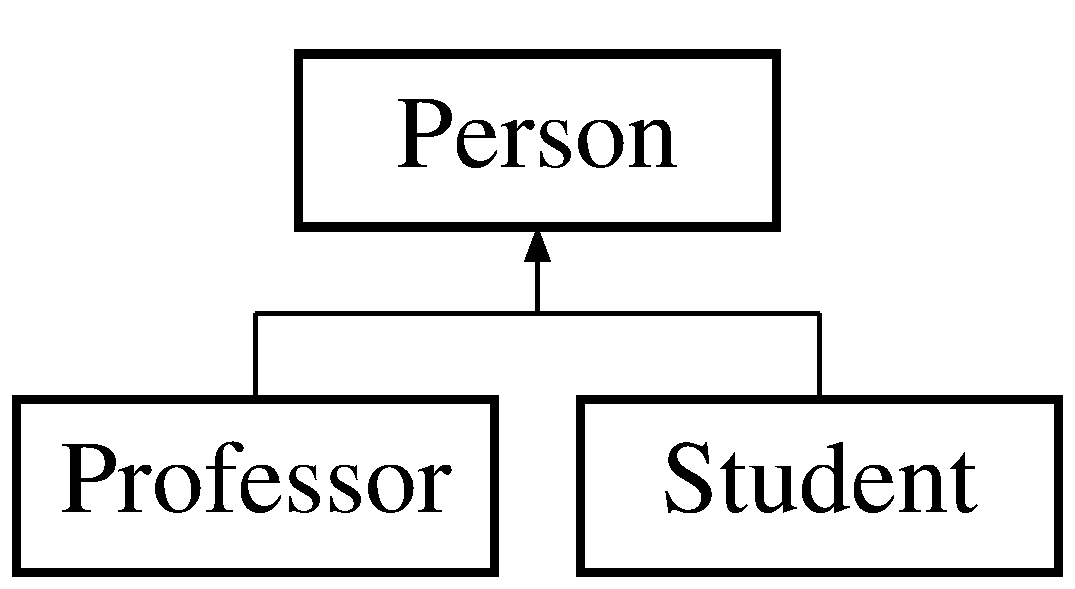
\includegraphics[height=2.000000cm]{class_person}
\end{center}
\end{figure}
\subsection*{Public Member Functions}
\begin{DoxyCompactItemize}
\item 
\hyperlink{class_person_a0397c6f89fafc12e738923f612bc41a3}{Person} ()
\begin{DoxyCompactList}\small\item\em Default constructor for \hyperlink{class_person}{Person} class. \end{DoxyCompactList}\item 
\hyperlink{class_person_a89a3ed74790668699f46f5cfbcd16bd0}{Person} (string \hyperlink{class_person_a669b64897b4d823a27bb5866368d4dfa}{name}, int \hyperlink{class_person_aec48a92f614a854ff380a15eb8e2f479}{id})
\begin{DoxyCompactList}\small\item\em Custom constructor for the person class. \end{DoxyCompactList}\item 
virtual \hyperlink{class_person_a6b5729bb56531c93312b1179c8ee4b71}{$\sim$\+Person} ()
\begin{DoxyCompactList}\small\item\em Destructor of \hyperlink{class_person}{Person} class. \end{DoxyCompactList}\item 
string \hyperlink{class_person_a9db2e2ccfc6cfa0d7979613ec2aaa922}{get\+Name} () const
\item 
void \hyperlink{class_person_a0f6294ead76bdac161bc71854799b09c}{set\+Name} (string new\+Name)
\begin{DoxyCompactList}\small\item\em Sets a new name for the person. \end{DoxyCompactList}\item 
void \hyperlink{class_person_ae08bf551df2688cd866c41b5d9cb8f1c}{set\+Id} (int \hyperlink{class_person_aec48a92f614a854ff380a15eb8e2f479}{id})
\begin{DoxyCompactList}\small\item\em Sets a new id for the person. \end{DoxyCompactList}\item 
int \hyperlink{class_person_afd0359228a09c4adcffe31f456046717}{get\+Id} ()
\item 
virtual void \hyperlink{class_person_a1f6361e735885ead2549717bb31d0437}{add\+New\+Title} (string title)
\begin{DoxyCompactList}\small\item\em Adds a new title to the person. \end{DoxyCompactList}\item 
virtual void \hyperlink{class_person_a14f687637476ef033a3c9b865e67fd69}{delete\+Title} (string title)
\begin{DoxyCompactList}\small\item\em Delete a title from a perosn. \end{DoxyCompactList}\end{DoxyCompactItemize}
\subsection*{Protected Attributes}
\begin{DoxyCompactItemize}
\item 
int \hyperlink{class_person_aec48a92f614a854ff380a15eb8e2f479}{id}
\item 
string \hyperlink{class_person_a669b64897b4d823a27bb5866368d4dfa}{name}
\item 
vector$<$ string $>$ \hyperlink{class_person_a162c1e6b3ce254b6bbffc0e947943031}{title\+Enun}
\end{DoxyCompactItemize}


\subsection{Constructor \& Destructor Documentation}
\mbox{\Hypertarget{class_person_a0397c6f89fafc12e738923f612bc41a3}\label{class_person_a0397c6f89fafc12e738923f612bc41a3}} 
\index{Person@{Person}!Person@{Person}}
\index{Person@{Person}!Person@{Person}}
\subsubsection{\texorpdfstring{Person()}{Person()}\hspace{0.1cm}{\footnotesize\ttfamily [1/2]}}
{\footnotesize\ttfamily Person\+::\+Person (\begin{DoxyParamCaption}{ }\end{DoxyParamCaption})}



Default constructor for \hyperlink{class_person}{Person} class. 

\mbox{\Hypertarget{class_person_a89a3ed74790668699f46f5cfbcd16bd0}\label{class_person_a89a3ed74790668699f46f5cfbcd16bd0}} 
\index{Person@{Person}!Person@{Person}}
\index{Person@{Person}!Person@{Person}}
\subsubsection{\texorpdfstring{Person()}{Person()}\hspace{0.1cm}{\footnotesize\ttfamily [2/2]}}
{\footnotesize\ttfamily Person\+::\+Person (\begin{DoxyParamCaption}\item[{string}]{name,  }\item[{int}]{id }\end{DoxyParamCaption})}



Custom constructor for the person class. 


\begin{DoxyParams}{Parameters}
{\em name} & Name of the person \\
\hline
{\em id} & Id of the person \\
\hline
\end{DoxyParams}
\mbox{\Hypertarget{class_person_a6b5729bb56531c93312b1179c8ee4b71}\label{class_person_a6b5729bb56531c93312b1179c8ee4b71}} 
\index{Person@{Person}!````~Person@{$\sim$\+Person}}
\index{````~Person@{$\sim$\+Person}!Person@{Person}}
\subsubsection{\texorpdfstring{$\sim$\+Person()}{~Person()}}
{\footnotesize\ttfamily virtual Person\+::$\sim$\+Person (\begin{DoxyParamCaption}{ }\end{DoxyParamCaption})\hspace{0.3cm}{\ttfamily [inline]}, {\ttfamily [virtual]}}



Destructor of \hyperlink{class_person}{Person} class. 



\subsection{Member Function Documentation}
\mbox{\Hypertarget{class_person_a1f6361e735885ead2549717bb31d0437}\label{class_person_a1f6361e735885ead2549717bb31d0437}} 
\index{Person@{Person}!add\+New\+Title@{add\+New\+Title}}
\index{add\+New\+Title@{add\+New\+Title}!Person@{Person}}
\subsubsection{\texorpdfstring{add\+New\+Title()}{addNewTitle()}}
{\footnotesize\ttfamily void Person\+::add\+New\+Title (\begin{DoxyParamCaption}\item[{string}]{title }\end{DoxyParamCaption})\hspace{0.3cm}{\ttfamily [virtual]}}



Adds a new title to the person. 


\begin{DoxyParams}{Parameters}
{\em title} & The new title to be added \\
\hline
\end{DoxyParams}


Reimplemented in \hyperlink{class_student_a616e34f2eebf885b3419bcd27e8f3840}{Student}.

\mbox{\Hypertarget{class_person_a14f687637476ef033a3c9b865e67fd69}\label{class_person_a14f687637476ef033a3c9b865e67fd69}} 
\index{Person@{Person}!delete\+Title@{delete\+Title}}
\index{delete\+Title@{delete\+Title}!Person@{Person}}
\subsubsection{\texorpdfstring{delete\+Title()}{deleteTitle()}}
{\footnotesize\ttfamily void Person\+::delete\+Title (\begin{DoxyParamCaption}\item[{string}]{title }\end{DoxyParamCaption})\hspace{0.3cm}{\ttfamily [virtual]}}



Delete a title from a perosn. 


\begin{DoxyParams}{Parameters}
{\em title} & The title to be deleted \\
\hline
\end{DoxyParams}


Reimplemented in \hyperlink{class_student_a16d2a2c6abe8aa9ce53a2a15c4656eee}{Student}.

\mbox{\Hypertarget{class_person_afd0359228a09c4adcffe31f456046717}\label{class_person_afd0359228a09c4adcffe31f456046717}} 
\index{Person@{Person}!get\+Id@{get\+Id}}
\index{get\+Id@{get\+Id}!Person@{Person}}
\subsubsection{\texorpdfstring{get\+Id()}{getId()}}
{\footnotesize\ttfamily int Person\+::get\+Id (\begin{DoxyParamCaption}{ }\end{DoxyParamCaption})}

\begin{DoxyReturn}{Returns}
The id of a person 
\end{DoxyReturn}
\mbox{\Hypertarget{class_person_a9db2e2ccfc6cfa0d7979613ec2aaa922}\label{class_person_a9db2e2ccfc6cfa0d7979613ec2aaa922}} 
\index{Person@{Person}!get\+Name@{get\+Name}}
\index{get\+Name@{get\+Name}!Person@{Person}}
\subsubsection{\texorpdfstring{get\+Name()}{getName()}}
{\footnotesize\ttfamily string Person\+::get\+Name (\begin{DoxyParamCaption}{ }\end{DoxyParamCaption}) const}

\begin{DoxyReturn}{Returns}
The name of the person 
\end{DoxyReturn}
\mbox{\Hypertarget{class_person_ae08bf551df2688cd866c41b5d9cb8f1c}\label{class_person_ae08bf551df2688cd866c41b5d9cb8f1c}} 
\index{Person@{Person}!set\+Id@{set\+Id}}
\index{set\+Id@{set\+Id}!Person@{Person}}
\subsubsection{\texorpdfstring{set\+Id()}{setId()}}
{\footnotesize\ttfamily void Person\+::set\+Id (\begin{DoxyParamCaption}\item[{int}]{id }\end{DoxyParamCaption})}



Sets a new id for the person. 


\begin{DoxyParams}{Parameters}
{\em id} & The new id for the person \\
\hline
\end{DoxyParams}
\mbox{\Hypertarget{class_person_a0f6294ead76bdac161bc71854799b09c}\label{class_person_a0f6294ead76bdac161bc71854799b09c}} 
\index{Person@{Person}!set\+Name@{set\+Name}}
\index{set\+Name@{set\+Name}!Person@{Person}}
\subsubsection{\texorpdfstring{set\+Name()}{setName()}}
{\footnotesize\ttfamily void Person\+::set\+Name (\begin{DoxyParamCaption}\item[{string}]{new\+Name }\end{DoxyParamCaption})}



Sets a new name for the person. 


\begin{DoxyParams}{Parameters}
{\em new\+Name} & The new name \\
\hline
\end{DoxyParams}


\subsection{Member Data Documentation}
\mbox{\Hypertarget{class_person_aec48a92f614a854ff380a15eb8e2f479}\label{class_person_aec48a92f614a854ff380a15eb8e2f479}} 
\index{Person@{Person}!id@{id}}
\index{id@{id}!Person@{Person}}
\subsubsection{\texorpdfstring{id}{id}}
{\footnotesize\ttfamily int Person\+::id\hspace{0.3cm}{\ttfamily [protected]}}

\mbox{\Hypertarget{class_person_a669b64897b4d823a27bb5866368d4dfa}\label{class_person_a669b64897b4d823a27bb5866368d4dfa}} 
\index{Person@{Person}!name@{name}}
\index{name@{name}!Person@{Person}}
\subsubsection{\texorpdfstring{name}{name}}
{\footnotesize\ttfamily string Person\+::name\hspace{0.3cm}{\ttfamily [protected]}}

\mbox{\Hypertarget{class_person_a162c1e6b3ce254b6bbffc0e947943031}\label{class_person_a162c1e6b3ce254b6bbffc0e947943031}} 
\index{Person@{Person}!title\+Enun@{title\+Enun}}
\index{title\+Enun@{title\+Enun}!Person@{Person}}
\subsubsection{\texorpdfstring{title\+Enun}{titleEnun}}
{\footnotesize\ttfamily vector$<$string$>$ Person\+::title\+Enun\hspace{0.3cm}{\ttfamily [protected]}}



The documentation for this class was generated from the following files\+:\begin{DoxyCompactItemize}
\item 
\hyperlink{student_8h}{student.\+h}\item 
\hyperlink{student_8cpp}{student.\+cpp}\end{DoxyCompactItemize}

\hypertarget{class_professor}{}\section{Professor Class Reference}
\label{class_professor}\index{Professor@{Professor}}


{\ttfamily \#include $<$student.\+h$>$}

Inheritance diagram for Professor\+:\begin{figure}[H]
\begin{center}
\leavevmode
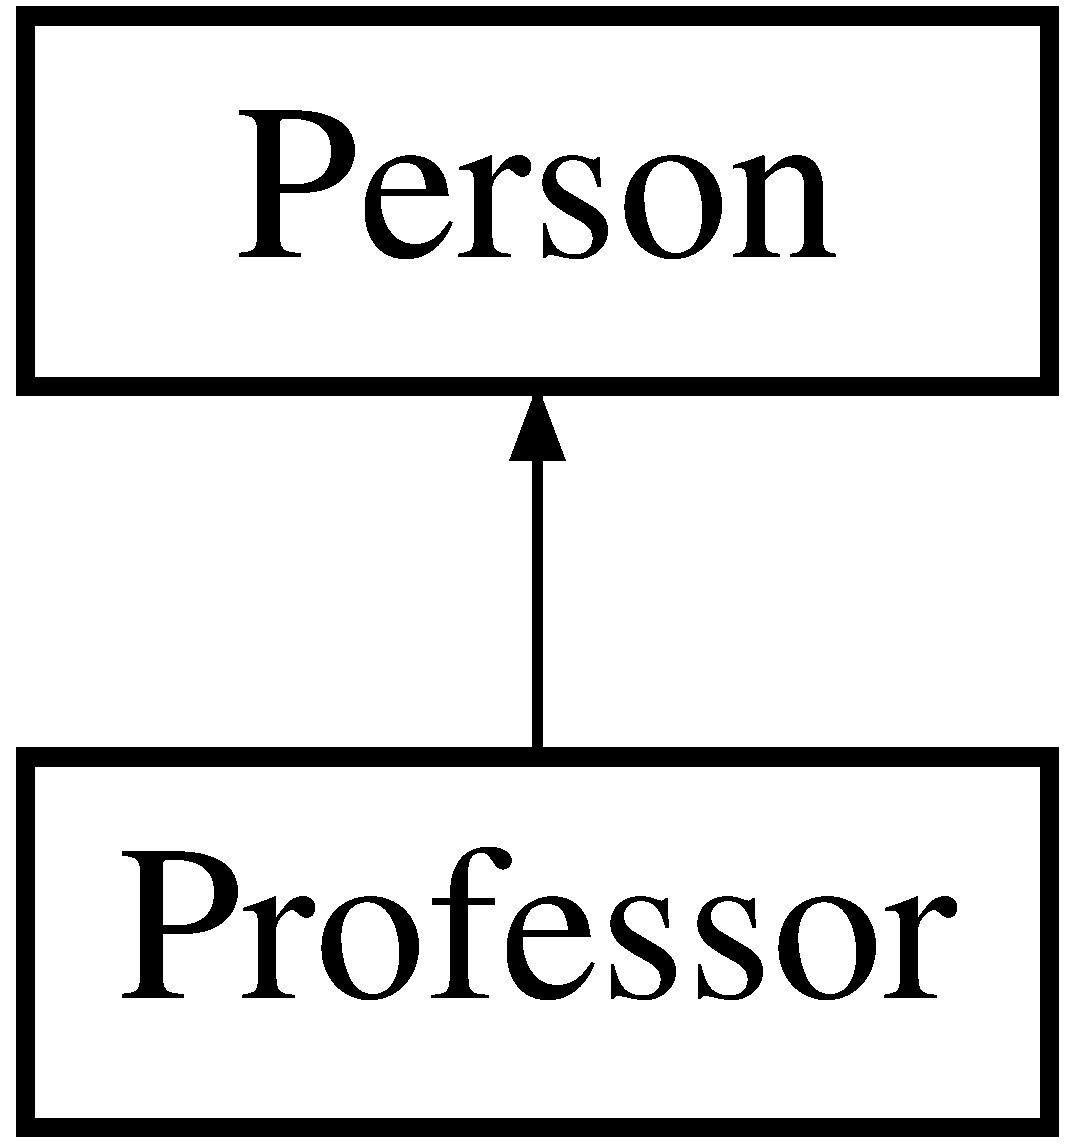
\includegraphics[height=2.000000cm]{class_professor}
\end{center}
\end{figure}
\subsection*{Public Member Functions}
\begin{DoxyCompactItemize}
\item 
\hyperlink{class_professor_ac6d4e54caf399a841888e60b54eed4c3}{Professor} ()
\begin{DoxyCompactList}\small\item\em Default constructor for class \hyperlink{class_student}{Student}. \end{DoxyCompactList}\item 
\hyperlink{class_professor_ac264bd1b8657897edf63ecb535315ab7}{Professor} (string \hyperlink{class_person_a669b64897b4d823a27bb5866368d4dfa}{name}, int \hyperlink{class_person_aec48a92f614a854ff380a15eb8e2f479}{id})
\begin{DoxyCompactList}\small\item\em Custom constructor for the professor class. \end{DoxyCompactList}\item 
virtual \hyperlink{class_professor_ac3b5cfd3e0016f25f4c2c194ccd593d8}{$\sim$\+Professor} ()
\begin{DoxyCompactList}\small\item\em Destructor. \end{DoxyCompactList}\item 
string \hyperlink{class_professor_ab82335224aa182146ec08b3f9cc4e2b4}{print\+Info\+Professor} ()
\end{DoxyCompactItemize}
\subsection*{Additional Inherited Members}


\subsection{Constructor \& Destructor Documentation}
\mbox{\Hypertarget{class_professor_ac6d4e54caf399a841888e60b54eed4c3}\label{class_professor_ac6d4e54caf399a841888e60b54eed4c3}} 
\index{Professor@{Professor}!Professor@{Professor}}
\index{Professor@{Professor}!Professor@{Professor}}
\subsubsection{\texorpdfstring{Professor()}{Professor()}\hspace{0.1cm}{\footnotesize\ttfamily [1/2]}}
{\footnotesize\ttfamily Professor\+::\+Professor (\begin{DoxyParamCaption}{ }\end{DoxyParamCaption})}



Default constructor for class \hyperlink{class_student}{Student}. 

\mbox{\Hypertarget{class_professor_ac264bd1b8657897edf63ecb535315ab7}\label{class_professor_ac264bd1b8657897edf63ecb535315ab7}} 
\index{Professor@{Professor}!Professor@{Professor}}
\index{Professor@{Professor}!Professor@{Professor}}
\subsubsection{\texorpdfstring{Professor()}{Professor()}\hspace{0.1cm}{\footnotesize\ttfamily [2/2]}}
{\footnotesize\ttfamily Professor\+::\+Professor (\begin{DoxyParamCaption}\item[{string}]{name,  }\item[{int}]{id }\end{DoxyParamCaption})}



Custom constructor for the professor class. 


\begin{DoxyParams}{Parameters}
{\em name} & The name of the professor \\
\hline
{\em id} & Id for the new professor \\
\hline
\end{DoxyParams}
\mbox{\Hypertarget{class_professor_ac3b5cfd3e0016f25f4c2c194ccd593d8}\label{class_professor_ac3b5cfd3e0016f25f4c2c194ccd593d8}} 
\index{Professor@{Professor}!````~Professor@{$\sim$\+Professor}}
\index{````~Professor@{$\sim$\+Professor}!Professor@{Professor}}
\subsubsection{\texorpdfstring{$\sim$\+Professor()}{~Professor()}}
{\footnotesize\ttfamily virtual Professor\+::$\sim$\+Professor (\begin{DoxyParamCaption}{ }\end{DoxyParamCaption})\hspace{0.3cm}{\ttfamily [inline]}, {\ttfamily [virtual]}}



Destructor. 



\subsection{Member Function Documentation}
\mbox{\Hypertarget{class_professor_ab82335224aa182146ec08b3f9cc4e2b4}\label{class_professor_ab82335224aa182146ec08b3f9cc4e2b4}} 
\index{Professor@{Professor}!print\+Info\+Professor@{print\+Info\+Professor}}
\index{print\+Info\+Professor@{print\+Info\+Professor}!Professor@{Professor}}
\subsubsection{\texorpdfstring{print\+Info\+Professor()}{printInfoProfessor()}}
{\footnotesize\ttfamily string Professor\+::print\+Info\+Professor (\begin{DoxyParamCaption}{ }\end{DoxyParamCaption})}

\begin{DoxyReturn}{Returns}
String containing the info of the professor 
\end{DoxyReturn}


The documentation for this class was generated from the following files\+:\begin{DoxyCompactItemize}
\item 
\hyperlink{student_8h}{student.\+h}\item 
\hyperlink{student_8cpp}{student.\+cpp}\end{DoxyCompactItemize}

\hypertarget{class_student}{}\section{Student Class Reference}
\label{class_student}\index{Student@{Student}}


{\ttfamily \#include $<$student.\+h$>$}

Inheritance diagram for Student\+:\begin{figure}[H]
\begin{center}
\leavevmode
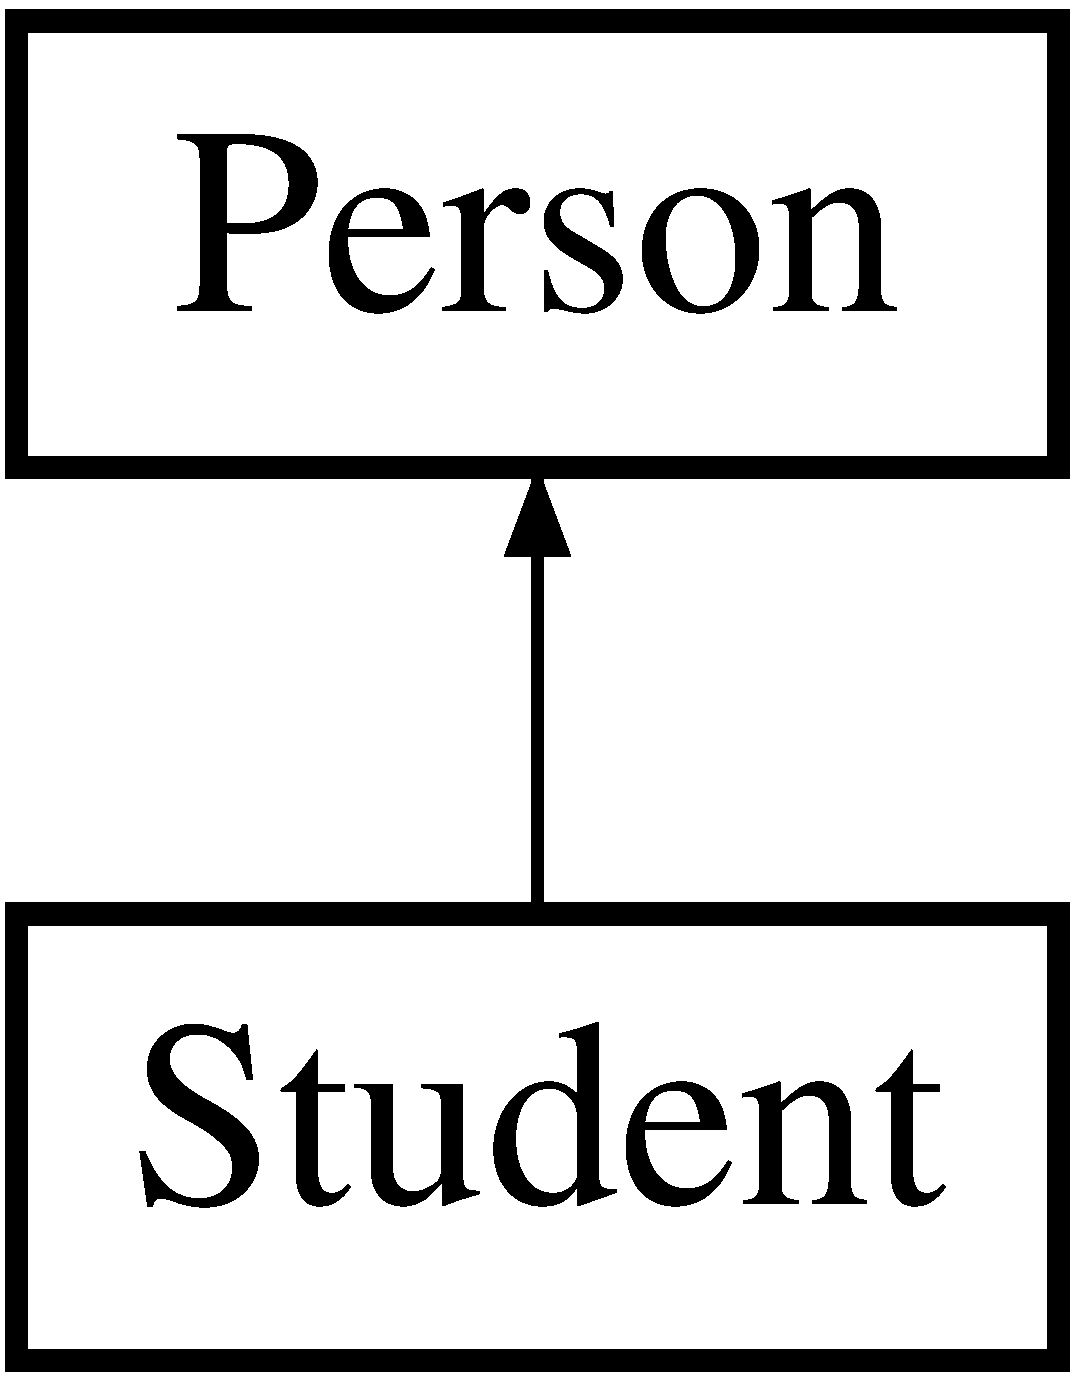
\includegraphics[height=2.000000cm]{class_student}
\end{center}
\end{figure}
\subsection*{Public Member Functions}
\begin{DoxyCompactItemize}
\item 
\hyperlink{class_student_af9168cedbfa5565cf0b20c1a9d3f5c9d}{Student} ()
\begin{DoxyCompactList}\small\item\em Default constructor for class \hyperlink{class_student}{Student}. \end{DoxyCompactList}\item 
\hyperlink{class_student_afc317f470d694b6ef52387a4e21a1e08}{Student} (string \hyperlink{class_person_a669b64897b4d823a27bb5866368d4dfa}{name}, int \hyperlink{class_person_aec48a92f614a854ff380a15eb8e2f479}{id})
\begin{DoxyCompactList}\small\item\em Custom constructor for the class \hyperlink{class_student}{Student}. \end{DoxyCompactList}\item 
virtual \hyperlink{class_student_a71f6d37e021e98dff29ffe67bfac6ce1}{$\sim$\+Student} ()
\begin{DoxyCompactList}\small\item\em Destructor of \hyperlink{class_student}{Student}. \end{DoxyCompactList}\item 
vector$<$ int $>$ \hyperlink{class_student_aff1ed57b8df6e9a3a43a32dc99923b34}{get\+Marks} ()
\item 
int \hyperlink{class_student_a05a0feee9294d3502af003fb65e56adf}{get\+Mark} (string title)
\item 
void \hyperlink{class_student_ad197a15a65230e59d0a690a49738e9af}{set\+Mark} (int mark, string title)
\begin{DoxyCompactList}\small\item\em Sets a mark for a student on a certain title. \end{DoxyCompactList}\item 
string \hyperlink{class_student_a4b566cc6bf1a725ca1569f306046b16b}{print\+Info\+Student} ()
\item 
void \hyperlink{class_student_a616e34f2eebf885b3419bcd27e8f3840}{add\+New\+Title} (string title)
\begin{DoxyCompactList}\small\item\em Adds a new title to the person. \end{DoxyCompactList}\item 
void \hyperlink{class_student_a16d2a2c6abe8aa9ce53a2a15c4656eee}{delete\+Title} (string title)
\begin{DoxyCompactList}\small\item\em Deletes a title from the student. \end{DoxyCompactList}\end{DoxyCompactItemize}
\subsection*{Additional Inherited Members}


\subsection{Constructor \& Destructor Documentation}
\mbox{\Hypertarget{class_student_af9168cedbfa5565cf0b20c1a9d3f5c9d}\label{class_student_af9168cedbfa5565cf0b20c1a9d3f5c9d}} 
\index{Student@{Student}!Student@{Student}}
\index{Student@{Student}!Student@{Student}}
\subsubsection{\texorpdfstring{Student()}{Student()}\hspace{0.1cm}{\footnotesize\ttfamily [1/2]}}
{\footnotesize\ttfamily Student\+::\+Student (\begin{DoxyParamCaption}{ }\end{DoxyParamCaption})}



Default constructor for class \hyperlink{class_student}{Student}. 

\mbox{\Hypertarget{class_student_afc317f470d694b6ef52387a4e21a1e08}\label{class_student_afc317f470d694b6ef52387a4e21a1e08}} 
\index{Student@{Student}!Student@{Student}}
\index{Student@{Student}!Student@{Student}}
\subsubsection{\texorpdfstring{Student()}{Student()}\hspace{0.1cm}{\footnotesize\ttfamily [2/2]}}
{\footnotesize\ttfamily Student\+::\+Student (\begin{DoxyParamCaption}\item[{string}]{name,  }\item[{int}]{id }\end{DoxyParamCaption})}



Custom constructor for the class \hyperlink{class_student}{Student}. 


\begin{DoxyParams}{Parameters}
{\em name} & The name of the student \\
\hline
{\em id} & The id of the student \\
\hline
\end{DoxyParams}
\mbox{\Hypertarget{class_student_a71f6d37e021e98dff29ffe67bfac6ce1}\label{class_student_a71f6d37e021e98dff29ffe67bfac6ce1}} 
\index{Student@{Student}!````~Student@{$\sim$\+Student}}
\index{````~Student@{$\sim$\+Student}!Student@{Student}}
\subsubsection{\texorpdfstring{$\sim$\+Student()}{~Student()}}
{\footnotesize\ttfamily virtual Student\+::$\sim$\+Student (\begin{DoxyParamCaption}{ }\end{DoxyParamCaption})\hspace{0.3cm}{\ttfamily [inline]}, {\ttfamily [virtual]}}



Destructor of \hyperlink{class_student}{Student}. 



\subsection{Member Function Documentation}
\mbox{\Hypertarget{class_student_a616e34f2eebf885b3419bcd27e8f3840}\label{class_student_a616e34f2eebf885b3419bcd27e8f3840}} 
\index{Student@{Student}!add\+New\+Title@{add\+New\+Title}}
\index{add\+New\+Title@{add\+New\+Title}!Student@{Student}}
\subsubsection{\texorpdfstring{add\+New\+Title()}{addNewTitle()}}
{\footnotesize\ttfamily void Student\+::add\+New\+Title (\begin{DoxyParamCaption}\item[{string}]{title }\end{DoxyParamCaption})\hspace{0.3cm}{\ttfamily [virtual]}}



Adds a new title to the person. 


\begin{DoxyParams}{Parameters}
{\em title} & The new title to be added \\
\hline
\end{DoxyParams}


Reimplemented from \hyperlink{class_person_a1f6361e735885ead2549717bb31d0437}{Person}.

\mbox{\Hypertarget{class_student_a16d2a2c6abe8aa9ce53a2a15c4656eee}\label{class_student_a16d2a2c6abe8aa9ce53a2a15c4656eee}} 
\index{Student@{Student}!delete\+Title@{delete\+Title}}
\index{delete\+Title@{delete\+Title}!Student@{Student}}
\subsubsection{\texorpdfstring{delete\+Title()}{deleteTitle()}}
{\footnotesize\ttfamily void Student\+::delete\+Title (\begin{DoxyParamCaption}\item[{string}]{title }\end{DoxyParamCaption})\hspace{0.3cm}{\ttfamily [virtual]}}



Deletes a title from the student. 



Reimplemented from \hyperlink{class_person_a14f687637476ef033a3c9b865e67fd69}{Person}.

\mbox{\Hypertarget{class_student_a05a0feee9294d3502af003fb65e56adf}\label{class_student_a05a0feee9294d3502af003fb65e56adf}} 
\index{Student@{Student}!get\+Mark@{get\+Mark}}
\index{get\+Mark@{get\+Mark}!Student@{Student}}
\subsubsection{\texorpdfstring{get\+Mark()}{getMark()}}
{\footnotesize\ttfamily int Student\+::get\+Mark (\begin{DoxyParamCaption}\item[{string}]{title }\end{DoxyParamCaption})}

\begin{DoxyReturn}{Returns}
The mark of the student on a certain title(g.\+p.) 
\end{DoxyReturn}

\begin{DoxyParams}{Parameters}
{\em title} & Title of the enunciation \\
\hline
\end{DoxyParams}
\mbox{\Hypertarget{class_student_aff1ed57b8df6e9a3a43a32dc99923b34}\label{class_student_aff1ed57b8df6e9a3a43a32dc99923b34}} 
\index{Student@{Student}!get\+Marks@{get\+Marks}}
\index{get\+Marks@{get\+Marks}!Student@{Student}}
\subsubsection{\texorpdfstring{get\+Marks()}{getMarks()}}
{\footnotesize\ttfamily vector$<$ int $>$ Student\+::get\+Marks (\begin{DoxyParamCaption}{ }\end{DoxyParamCaption})}

\begin{DoxyReturn}{Returns}
Vector of marks of the student 
\end{DoxyReturn}
\mbox{\Hypertarget{class_student_a4b566cc6bf1a725ca1569f306046b16b}\label{class_student_a4b566cc6bf1a725ca1569f306046b16b}} 
\index{Student@{Student}!print\+Info\+Student@{print\+Info\+Student}}
\index{print\+Info\+Student@{print\+Info\+Student}!Student@{Student}}
\subsubsection{\texorpdfstring{print\+Info\+Student()}{printInfoStudent()}}
{\footnotesize\ttfamily string Student\+::print\+Info\+Student (\begin{DoxyParamCaption}{ }\end{DoxyParamCaption})}

\begin{DoxyReturn}{Returns}
String containing the info of the student 
\end{DoxyReturn}
\mbox{\Hypertarget{class_student_ad197a15a65230e59d0a690a49738e9af}\label{class_student_ad197a15a65230e59d0a690a49738e9af}} 
\index{Student@{Student}!set\+Mark@{set\+Mark}}
\index{set\+Mark@{set\+Mark}!Student@{Student}}
\subsubsection{\texorpdfstring{set\+Mark()}{setMark()}}
{\footnotesize\ttfamily void Student\+::set\+Mark (\begin{DoxyParamCaption}\item[{int}]{mark,  }\item[{string}]{title }\end{DoxyParamCaption})}



Sets a mark for a student on a certain title. 


\begin{DoxyParams}{Parameters}
{\em mark} & Mark to be added \\
\hline
{\em title} & Title of the enunciation \\
\hline
\end{DoxyParams}


The documentation for this class was generated from the following files\+:\begin{DoxyCompactItemize}
\item 
\hyperlink{student_8h}{student.\+h}\item 
\hyperlink{student_8cpp}{student.\+cpp}\end{DoxyCompactItemize}

\chapter{File Documentation}
\hypertarget{_b_s_t_8h}{}\section{B\+S\+T.\+h File Reference}
\label{_b_s_t_8h}\index{B\+S\+T.\+h@{B\+S\+T.\+h}}
{\ttfamily \#include $<$iostream$>$}\newline
{\ttfamily \#include $<$stack$>$}\newline
{\ttfamily \#include $<$queue$>$}\newline
\subsection*{Classes}
\begin{DoxyCompactItemize}
\item 
class \hyperlink{class_b_s_t_itr_in}{B\+S\+T\+Itr\+In$<$ Comparable $>$}
\item 
class \hyperlink{class_b_s_t_itr_pre}{B\+S\+T\+Itr\+Pre$<$ Comparable $>$}
\item 
class \hyperlink{class_b_s_t_itr_post}{B\+S\+T\+Itr\+Post$<$ Comparable $>$}
\item 
class \hyperlink{class_b_s_t_itr_level}{B\+S\+T\+Itr\+Level$<$ Comparable $>$}
\item 
class \hyperlink{class_b_s_t}{B\+S\+T$<$ Comparable $>$}
\item 
class \hyperlink{class_binary_node}{Binary\+Node$<$ Comparable $>$}
\item 
class \hyperlink{class_b_s_t}{B\+S\+T$<$ Comparable $>$}
\item 
class \hyperlink{class_b_s_t_itr_post}{B\+S\+T\+Itr\+Post$<$ Comparable $>$}
\item 
class \hyperlink{class_b_s_t_itr_pre}{B\+S\+T\+Itr\+Pre$<$ Comparable $>$}
\item 
class \hyperlink{class_b_s_t_itr_in}{B\+S\+T\+Itr\+In$<$ Comparable $>$}
\item 
class \hyperlink{class_b_s_t_itr_level}{B\+S\+T\+Itr\+Level$<$ Comparable $>$}
\end{DoxyCompactItemize}

\hypertarget{enunciation_8cpp}{}\section{enunciation.\+cpp File Reference}
\label{enunciation_8cpp}\index{enunciation.\+cpp@{enunciation.\+cpp}}
{\ttfamily \#include \char`\"{}enunciation.\+h\char`\"{}}\newline
{\ttfamily \#include \char`\"{}occurrence.\+h\char`\"{}}\newline
{\ttfamily \#include \char`\"{}insertion\+Sort.\+h\char`\"{}}\newline

\hypertarget{enunciation_8h}{}\section{enunciation.\+h File Reference}
\label{enunciation_8h}\index{enunciation.\+h@{enunciation.\+h}}
{\ttfamily \#include $<$iostream$>$}\newline
{\ttfamily \#include $<$string$>$}\newline
{\ttfamily \#include $<$vector$>$}\newline
{\ttfamily \#include $<$fstream$>$}\newline
{\ttfamily \#include $<$cstdlib$>$}\newline
{\ttfamily \#include $<$sstream$>$}\newline
{\ttfamily \#include \char`\"{}occurrence.\+h\char`\"{}}\newline
\subsection*{Classes}
\begin{DoxyCompactItemize}
\item 
class \hyperlink{class_enunciation}{Enunciation}
\item 
class \hyperlink{class_enunciation_research}{Enunciation\+Research}
\item 
class \hyperlink{class_enunciation_analysis}{Enunciation\+Analysis}
\item 
class \hyperlink{class_enunciation_development}{Enunciation\+Development}
\end{DoxyCompactItemize}

\hypertarget{general_8cpp}{}\section{general.\+cpp File Reference}
\label{general_8cpp}\index{general.\+cpp@{general.\+cpp}}
{\ttfamily \#include $<$iostream$>$}\newline
{\ttfamily \#include $<$vector$>$}\newline
{\ttfamily \#include $<$unistd.\+h$>$}\newline
{\ttfamily \#include $<$string$>$}\newline
{\ttfamily \#include $<$queue$>$}\newline
{\ttfamily \#include $<$ctime$>$}\newline
{\ttfamily \#include \char`\"{}enunciation.\+h\char`\"{}}\newline
{\ttfamily \#include \char`\"{}insertion\+Sort.\+h\char`\"{}}\newline
{\ttfamily \#include \char`\"{}group\+Project.\+h\char`\"{}}\newline
\subsection*{Classes}
\begin{DoxyCompactItemize}
\item 
struct \hyperlink{structgroup_project_hash}{group\+Project\+Hash}
\item 
class \hyperlink{classgeneral}{general}
\end{DoxyCompactItemize}
\subsection*{Typedefs}
\begin{DoxyCompactItemize}
\item 
typedef tr1\+::unordered\+\_\+set$<$ \hyperlink{classgroup_project}{group\+Project} $\ast$, \hyperlink{structgroup_project_hash}{group\+Project\+Hash}, \hyperlink{structgroup_project_hash}{group\+Project\+Hash} $>$ \hyperlink{general_8cpp_a0fc3a756eb97ca669104c846b7507f6d}{tab\+H\+Project}
\item 
typedef priority\+\_\+queue$<$ \hyperlink{classgroup_project}{group\+Project} $\ast$ $>$ \hyperlink{general_8cpp_aa812d17abc272e39f0dffeb86e73f7a6}{H\+E\+A\+P\+\_\+\+GP}
\end{DoxyCompactItemize}
\subsection*{Functions}
\begin{DoxyCompactItemize}
\item 
int \hyperlink{general_8cpp_ae66f6b31b5ad750f1fe042a706a4e3d4}{main} ()
\end{DoxyCompactItemize}


\subsection{Typedef Documentation}
\mbox{\Hypertarget{general_8cpp_aa812d17abc272e39f0dffeb86e73f7a6}\label{general_8cpp_aa812d17abc272e39f0dffeb86e73f7a6}} 
\index{general.\+cpp@{general.\+cpp}!H\+E\+A\+P\+\_\+\+GP@{H\+E\+A\+P\+\_\+\+GP}}
\index{H\+E\+A\+P\+\_\+\+GP@{H\+E\+A\+P\+\_\+\+GP}!general.\+cpp@{general.\+cpp}}
\subsubsection{\texorpdfstring{H\+E\+A\+P\+\_\+\+GP}{HEAP\_GP}}
{\footnotesize\ttfamily typedef priority\+\_\+queue$<$\hyperlink{classgroup_project}{group\+Project} $\ast$$>$ \hyperlink{general_8cpp_aa812d17abc272e39f0dffeb86e73f7a6}{H\+E\+A\+P\+\_\+\+GP}}

\mbox{\Hypertarget{general_8cpp_a0fc3a756eb97ca669104c846b7507f6d}\label{general_8cpp_a0fc3a756eb97ca669104c846b7507f6d}} 
\index{general.\+cpp@{general.\+cpp}!tab\+H\+Project@{tab\+H\+Project}}
\index{tab\+H\+Project@{tab\+H\+Project}!general.\+cpp@{general.\+cpp}}
\subsubsection{\texorpdfstring{tab\+H\+Project}{tabHProject}}
{\footnotesize\ttfamily typedef tr1\+::unordered\+\_\+set$<$\hyperlink{classgroup_project}{group\+Project}$\ast$, \hyperlink{structgroup_project_hash}{group\+Project\+Hash}, \hyperlink{structgroup_project_hash}{group\+Project\+Hash}$>$ \hyperlink{general_8cpp_a0fc3a756eb97ca669104c846b7507f6d}{tab\+H\+Project}}



\subsection{Function Documentation}
\mbox{\Hypertarget{general_8cpp_ae66f6b31b5ad750f1fe042a706a4e3d4}\label{general_8cpp_ae66f6b31b5ad750f1fe042a706a4e3d4}} 
\index{general.\+cpp@{general.\+cpp}!main@{main}}
\index{main@{main}!general.\+cpp@{general.\+cpp}}
\subsubsection{\texorpdfstring{main()}{main()}}
{\footnotesize\ttfamily int main (\begin{DoxyParamCaption}{ }\end{DoxyParamCaption})}


\hypertarget{group_project_8cpp}{}\section{group\+Project.\+cpp File Reference}
\label{group_project_8cpp}\index{group\+Project.\+cpp@{group\+Project.\+cpp}}
{\ttfamily \#include \char`\"{}group\+Project.\+h\char`\"{}}\newline
{\ttfamily \#include $<$sstream$>$}\newline

\hypertarget{group_project_8h}{}\section{group\+Project.\+h File Reference}
\label{group_project_8h}\index{group\+Project.\+h@{group\+Project.\+h}}
{\ttfamily \#include $<$fstream$>$}\newline
{\ttfamily \#include $<$iostream$>$}\newline
{\ttfamily \#include $<$tr1/unordered\+\_\+set$>$}\newline
{\ttfamily \#include \char`\"{}B\+S\+T.\+h\char`\"{}}\newline
{\ttfamily \#include \char`\"{}student.\+h\char`\"{}}\newline
\subsection*{Classes}
\begin{DoxyCompactItemize}
\item 
class \hyperlink{classgroup_project}{group\+Project}
\end{DoxyCompactItemize}

\hypertarget{insertion_sort_8h}{}\section{insertion\+Sort.\+h File Reference}
\label{insertion_sort_8h}\index{insertion\+Sort.\+h@{insertion\+Sort.\+h}}
{\ttfamily \#include $<$vector$>$}\newline
\subsection*{Functions}
\begin{DoxyCompactItemize}
\item 
{\footnotesize template$<$class Comparable $>$ }\\void \hyperlink{insertion_sort_8h_a2d750432a373f9dab8039bef160b71a0}{insertion\+Sort} (vector$<$ Comparable $>$ \&v)
\end{DoxyCompactItemize}


\subsection{Function Documentation}
\mbox{\Hypertarget{insertion_sort_8h_a2d750432a373f9dab8039bef160b71a0}\label{insertion_sort_8h_a2d750432a373f9dab8039bef160b71a0}} 
\index{insertion\+Sort.\+h@{insertion\+Sort.\+h}!insertion\+Sort@{insertion\+Sort}}
\index{insertion\+Sort@{insertion\+Sort}!insertion\+Sort.\+h@{insertion\+Sort.\+h}}
\subsubsection{\texorpdfstring{insertion\+Sort()}{insertionSort()}}
{\footnotesize\ttfamily template$<$class Comparable $>$ \\
void insertion\+Sort (\begin{DoxyParamCaption}\item[{vector$<$ Comparable $>$ \&}]{v }\end{DoxyParamCaption})}


\hypertarget{occurrence_8cpp}{}\section{occurrence.\+cpp File Reference}
\label{occurrence_8cpp}\index{occurrence.\+cpp@{occurrence.\+cpp}}
{\ttfamily \#include \char`\"{}occurrence.\+h\char`\"{}}\newline
{\ttfamily \#include $<$sstream$>$}\newline

\hypertarget{occurrence_8h}{}\section{occurrence.\+h File Reference}
\label{occurrence_8h}\index{occurrence.\+h@{occurrence.\+h}}
{\ttfamily \#include $<$iostream$>$}\newline
{\ttfamily \#include $<$vector$>$}\newline
{\ttfamily \#include \char`\"{}group\+Project.\+h\char`\"{}}\newline
\subsection*{Classes}
\begin{DoxyCompactItemize}
\item 
class \hyperlink{class_occurrence}{Occurrence}
\end{DoxyCompactItemize}

\hypertarget{sequential_search_8h}{}\section{sequential\+Search.\+h File Reference}
\label{sequential_search_8h}\index{sequential\+Search.\+h@{sequential\+Search.\+h}}
{\ttfamily \#include $<$vector$>$}\newline
\subsection*{Functions}
\begin{DoxyCompactItemize}
\item 
{\footnotesize template$<$class Comparable $>$ }\\int \hyperlink{sequential_search_8h_acd555ad1f1fc3b2011aab63641f98151}{sequential\+Search} (const vector$<$ Comparable $>$ \&v, Comparable x)
\end{DoxyCompactItemize}


\subsection{Function Documentation}
\mbox{\Hypertarget{sequential_search_8h_acd555ad1f1fc3b2011aab63641f98151}\label{sequential_search_8h_acd555ad1f1fc3b2011aab63641f98151}} 
\index{sequential\+Search.\+h@{sequential\+Search.\+h}!sequential\+Search@{sequential\+Search}}
\index{sequential\+Search@{sequential\+Search}!sequential\+Search.\+h@{sequential\+Search.\+h}}
\subsubsection{\texorpdfstring{sequential\+Search()}{sequentialSearch()}}
{\footnotesize\ttfamily template$<$class Comparable $>$ \\
int sequential\+Search (\begin{DoxyParamCaption}\item[{const vector$<$ Comparable $>$ \&}]{v,  }\item[{Comparable}]{x }\end{DoxyParamCaption})}


\hypertarget{student_8cpp}{}\section{student.\+cpp File Reference}
\label{student_8cpp}\index{student.\+cpp@{student.\+cpp}}
{\ttfamily \#include \char`\"{}student.\+h\char`\"{}}\newline
{\ttfamily \#include $<$iostream$>$}\newline
{\ttfamily \#include $<$sstream$>$}\newline
{\ttfamily \#include \char`\"{}sequential\+Search.\+h\char`\"{}}\newline

\hypertarget{student_8h}{}\section{student.\+h File Reference}
\label{student_8h}\index{student.\+h@{student.\+h}}
{\ttfamily \#include $<$iostream$>$}\newline
{\ttfamily \#include $<$vector$>$}\newline
\subsection*{Classes}
\begin{DoxyCompactItemize}
\item 
class \hyperlink{class_person}{Person}
\item 
class \hyperlink{class_student}{Student}
\item 
class \hyperlink{class_professor}{Professor}
\end{DoxyCompactItemize}

%--- End generated contents ---

% Index
\backmatter
\newpage
\phantomsection
\clearemptydoublepage
\addcontentsline{toc}{chapter}{Index}
\printindex

\end{document}
